\include{Macros/MacroFile1}

\documentclass[oneside,11pt]{Classes/myThesis}
%%%%%%%%%%%%%%%%%%%%%%%%%%%%%%%%%%%%%%%%%%%%%%%%%%%%%%
%%%%%%%%%%%%%%% file path for figures - add extra chapters as necessary %%%%%%%%%
%%%%%%%%%%%%%%%%%%%%%%%%%%%%%%%%%%%%%%%%%%%%%%%%%%%%%%
\graphicspath{{./Chapters/Chapter_1/Chapter_1_Fig/} 
	    		{./Chapters/Chapter1/Chapter1Figs/}
              {./Chapters/Chapter_2/Chapter_2_Fig/}
              {./Chapters/Chapter_3/Chapter_3_Fig/}
              {./Chapters/Chapter_4/Chapter_4_Fig/}
              {./Chapters/Chapter_4/IntersectionCore/method_fig/}
              {./Chapters/Chapter_4/IntersectionCore/}
              {./Appendix1/Fig/}
              {./Appendix2/Fig/}
              {./ThesisFigs/}}

%%%%%%%%%%%%%%%%%%%%%%%%%%%%%%%%%%%%%%%%%%%%%%%%%%%%%%
%%%%%%%%%%%%% Constants - fill these in for use throughout the thesis %%%%%%%%%%%%
%%%%%%%%%%%%%%%%%%%%%%%%%%%%%%%%%%%%%%%%%%%%%%%%%%%%%%
\newcommand{\theAuthor}{Edward Derek Lambert}
\newcommand{\authorEmail}{tsedl@leeds.ac.uk}
\newcommand{\myTitle}{Mathematical Modelling and Optimisation for Co-operative Intra-logistics Automated Vehicle Control}
%%%%%%%%%%%%%%%%%%%%%%%%%%%%%%%%%%%%%%%%%%%%%%%%%%%%%%
\pdfinfo { /Title  (\myTitle)
           /Creator (TeX)
           /Producer (pdfTeX)
           /Author (\theAuthor \authorEmail)
           /ModDate (D:\pdfdate)
           /CreationDate (D:\pdfdate)  %format D:YYYYMMDDhhmmss
           /Subject (Transport Studies)
           /Keywords (PhD, Thesis)}    
		\pdfcatalog { /PageMode (/UseOutlines)
                  /OpenAction (fitbh)  }

%%%%%%%%%%%%%%%%%%%%%%%%%%%%%%%%%%%%%%%%%%%%%%%%%%%%%%
%%%%%%%%%%%%% Title Page Information %%%%%%%%%%%%%%%%%%%%%%%%%%%%
%%%%%%%%%%%%%%%%%%%%%%%%%%%%%%%%%%%%%%%%%%%%%%%%%%%%%%
\title{\myTitle}
\author{\href{mailto:\authorEmail}{\theAuthor}}
\crest{\includegraphics[width=35mm]{Leeds_Crest.png}}
%%%%%%%%%%%%%%%%%%%%%%%%%%%%%%%%%%%%%%%%%%%%%%%%%%%%%%
%% Define these as empty to omit the two logos on the title page
%%%%%%%%%%%%%%%%%%%%%%%%%%%%%%%%%%%%%%%%%%%%%%%%%%%%%%
\logo{} %\includegraphics[width=50mm]{UoL_logo}} %University Logo
\deptlogo{} %\includegraphics[width=50mm]{UoL_logo}} % Institute Logo
%%%%%%%%%%%%%%%%%%%%%%%%%%%%%%%%%%%%%%%%%%%%%%%%%%%%%%
\collegeordept{\href{http://its.leeds.ac.uk}{Institute for Transport Studies}}
\university{\href{http://www.leeds.ac.uk}{University of Leeds}}

\degree{Doctor of Philosophy}
\degreedate{\monthdate\today}

%Different font in captions
%Different font in caption
%%%%%%%%%%%%%%%%%%%%%%%%%%%%%%%%%%%%%%%%%%%%%%%%%%%%%%
%%%%%%%%%%%%%%%% Optional Packages  %%%%%%%%%%%%%%%%%%%%%%%%%%%
%%%%%%%%%%%%%%%%%%%%%%%%%%%%%%%%%%%%%%%%%%%%%%%%%%%%%%
%\usepackage{StyleFiles/watermark}
%\usepackage{xspace}  %add a space after maths if not already there
%\usepackage{booktabs} %better tables
%\usepackage{rotating}  %rotating figures and tables
% \usepackage{array} %enhanced tables
%\usepackage{ctable} %include a figure command
%\usepackage{footnote}
%\usepackage{multirow} %for merging cells on tables
%\usepackage{times} % The "Times" font
%\usepackage{Utopia} % The "Utopia" font
\usepackage{bm}
\usepackage{amsmath}
%\usepackage[ruled,vlined]{algorithm2e} -> ifoddpage.sty not found error
\usepackage{algorithmic}% -> looks rubbish
\usepackage[final]{pdfpages} % for lazy appendix
\linespread{1.3} %1.5 line spacing

\begin{document}
%\baselineskip=18pt plus1pt

\maketitle
%set the number of sectioning levels that get number and appear in the contents
\setcounter{secnumdepth}{2}
\setcounter{tocdepth}{2}
\pagenumbering{roman}
\frontmatter
%%%%%%%%%%%%%%%%%%%%%%%%%%%%%%%%%%%%%%%%%%%%%%%%%%%%%%
%%%%%%%%%%%% Include sections are required, or comment out to skip over %%%%%%%%%
%%%%%%%%%%%%%%%%%%%%%%%%%%%%%%%%%%%%%%%%%%%%%%%%%%%%%%
%\include{Dedication/dedication}
\include{IPStatement/ipstatement}
% Thesis Acknowledgements ------------------------------------------------


%\begin{acknowledgementslong} %uncommenting this line, gives a different acknowledgements heading
\begin{acknowledgements}      %this creates the heading for the acknowlegments

\setlength{\parindent}{17.62482pt}
\setlength{\parskip}{0.0pt plus 1.0pt}

%Thanks to Dr. Dave Barnett for introducing me to Automated Guided Vehicles the clothoid curve, and teaching me how to write software. Thanks to Dr Martin Davies and Dr Paul Rivers and everyone at Guidance Automation Ltd for answering all my stupid questions. Thanks to Prof Rich Romano and Prof David Watling for keeping me on track, guarding my time and teaching me how to be a better academic. 
Thanks everyone. 

\end{acknowledgements}
%\end{acknowledgmentslong}

% ------------------------------------------------------------------------

%%% Local Variables: 
%%% mode: latex
%%% TeX-master: "../thesis"
%%% End: 

\include{Abstract/abstract}
\newpage
\tableofcontents
\newpage
\listoffigures
\newpage
\listoftables
\newpage
\include{Abbreviations/Abbreviations}
%\include{Common_Symbols/Common_Symbols}

\mainmatter

\pagenumbering{arabic}
%% file path for chapter tex files 
%=== Chapter One ===
\chapter{Combined Introduction}
\section{Intra-logistics}
Intra-logistics concerns the movement of goods within distribution warehouses. Here, homogeneous stock lines are combined and transported into heterogeneous customer boxes for delivery. Each customer order may be stored in a Warehouse Management Database, and new online orders may arrive at any time during operation. 
%=== Chapter One ===
\chapter{Combined Literature Review}

%\ifpdf
%    \graphicspath{{Chapter1/Chapter1Figs/PNG/}{Chapter1/Chapter1/PDF/}{Chapter1/Chapter1Figs/}}
%\else
%    \graphicspath{{Chapter1/Chapter1Figs/EPS/}{Chapter1/Chapter1/}}
%\fi

\section{Robotic Path Planning}

\subsection{Introduction}
There has been more than 50 years of progress in robotic path planning, at least a substantial proportion regarding the paths of wheeled mobile robots moving in a two dimensional plane. The goal of this review is not to provide a complete reference, but to justify a certain approach to the problem which is appropriate for the domain of car-like automated vehicles moving goods in automated warehouses.

The central problem is that of a vehicle which follows a defined reference path through a known environment. In some situations the environment may change in such a way that the reference path is no longer feasible. In this case a new path must be generated based on the local information available to the vehicle, and that available from communicating vehicles. This is called Adaptive Local Planning. There are certain requirements for Adaptive Local Planning which are important for the automated warehouse domain more than others. The review reveals that is is more useful to focus on trajectories for the adaptive planning. The trajectories must be feasible in the sense that they meet obstacle avoidance constraints, and in the sense that they meet differential constraints arising from dynamic considerations of the vehicles motion. Furthermore, a guarantee that a path will be found if one exists is a desirable property. It is also desirable for the algorithm to generate a path in a consistent execution time so that the path is always available to the motion control system. In many cases these are conflicting goals: a planner with a hard time limit will not be able to search all possibilities exhaustively. 

\subsection{Planning Architectures}

\cite{Schwarting2018} divide architectures of automated vehicles into three broad categories: Traditional; Behaviour aware, and End-to-end machine learning. Traditional approaches are hierarchical, breaking the problem down into layers including perception, behaviour choice, motion planning, and feedback control. A variety of techniques can then be used at each layer. Perception covers the creation of a representation of the environment from various sensors and lies outside the scope of this review. In the DARPA Urban Challenge contestants this often consisted of a state machine which used expert rules to decide the best manoeuvre such as change lane to be executed by the motion planner \cite{Urmson2008}. The motion planner generated detailed action sequences - trajectories which provide the reference for the feedback control component. 


%\begin{figure}[htbp]
%\begin{center}
%%  \mbox{
%%     \subfigure[]{{\includegraphics[width=0.3\columnwidth, angle=-0]{BehaviourAwareFlowChart}} }
%%     \subfigure[]{{\includegraphics[width=0.3\columnwidth, angle=-0]{BehaviourAwareFlowChart}}}
%%     \subfigure[]{{\includegraphics[width=0.3\columnwidth, angle=-0]{BehaviourAwareFlowChart}}}
%%       }
%\label{fig:broad_categories}
%\end{center}
%\end{figure}

\begin{figure}[ht]
  \begin{center}
	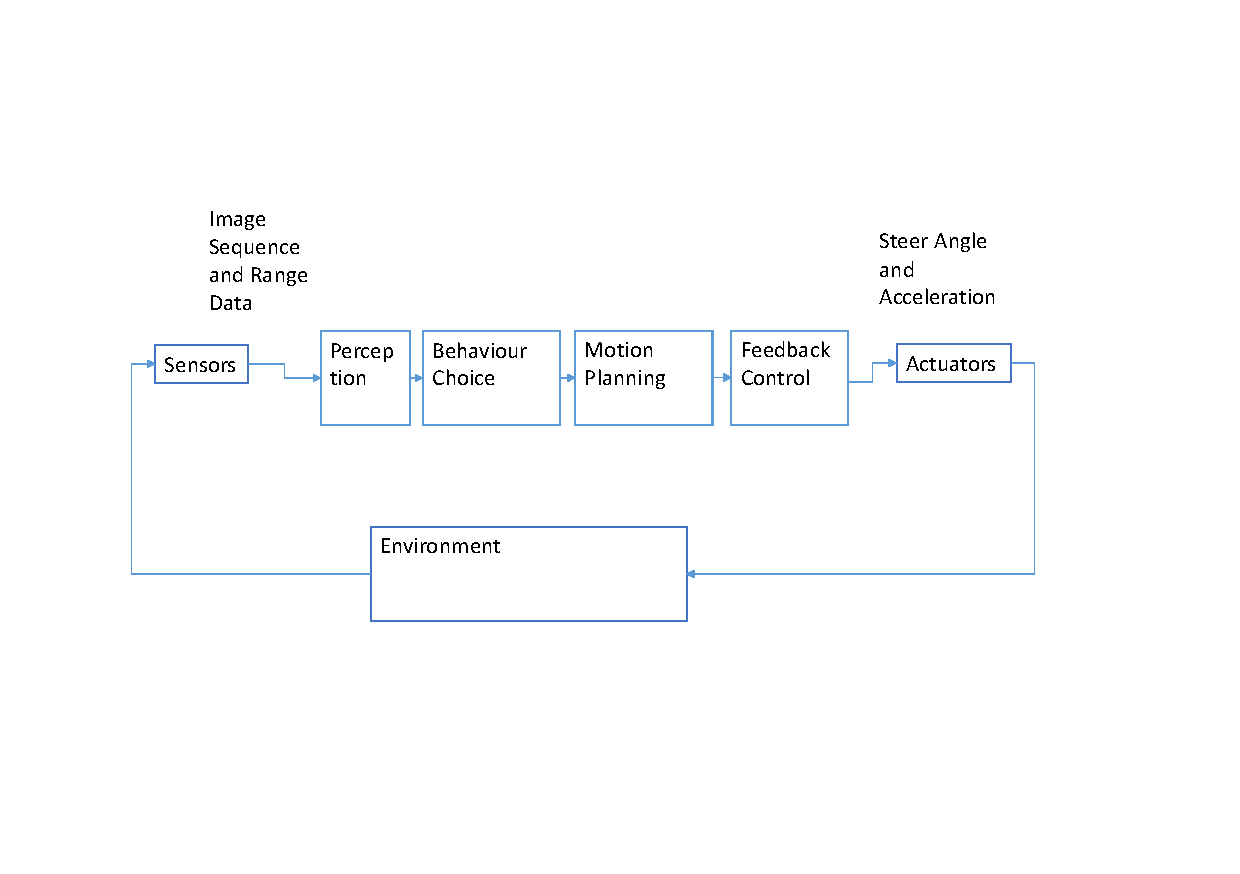
\includegraphics[width=\columnwidth, angle=-0]{HierarchFlowChart}
	\caption{Logical flow of hierarchical planning}
	\label{fig:hierarch_flow}
  \end{center}
\end{figure}
\begin{figure}[ht]
  \begin{center}
	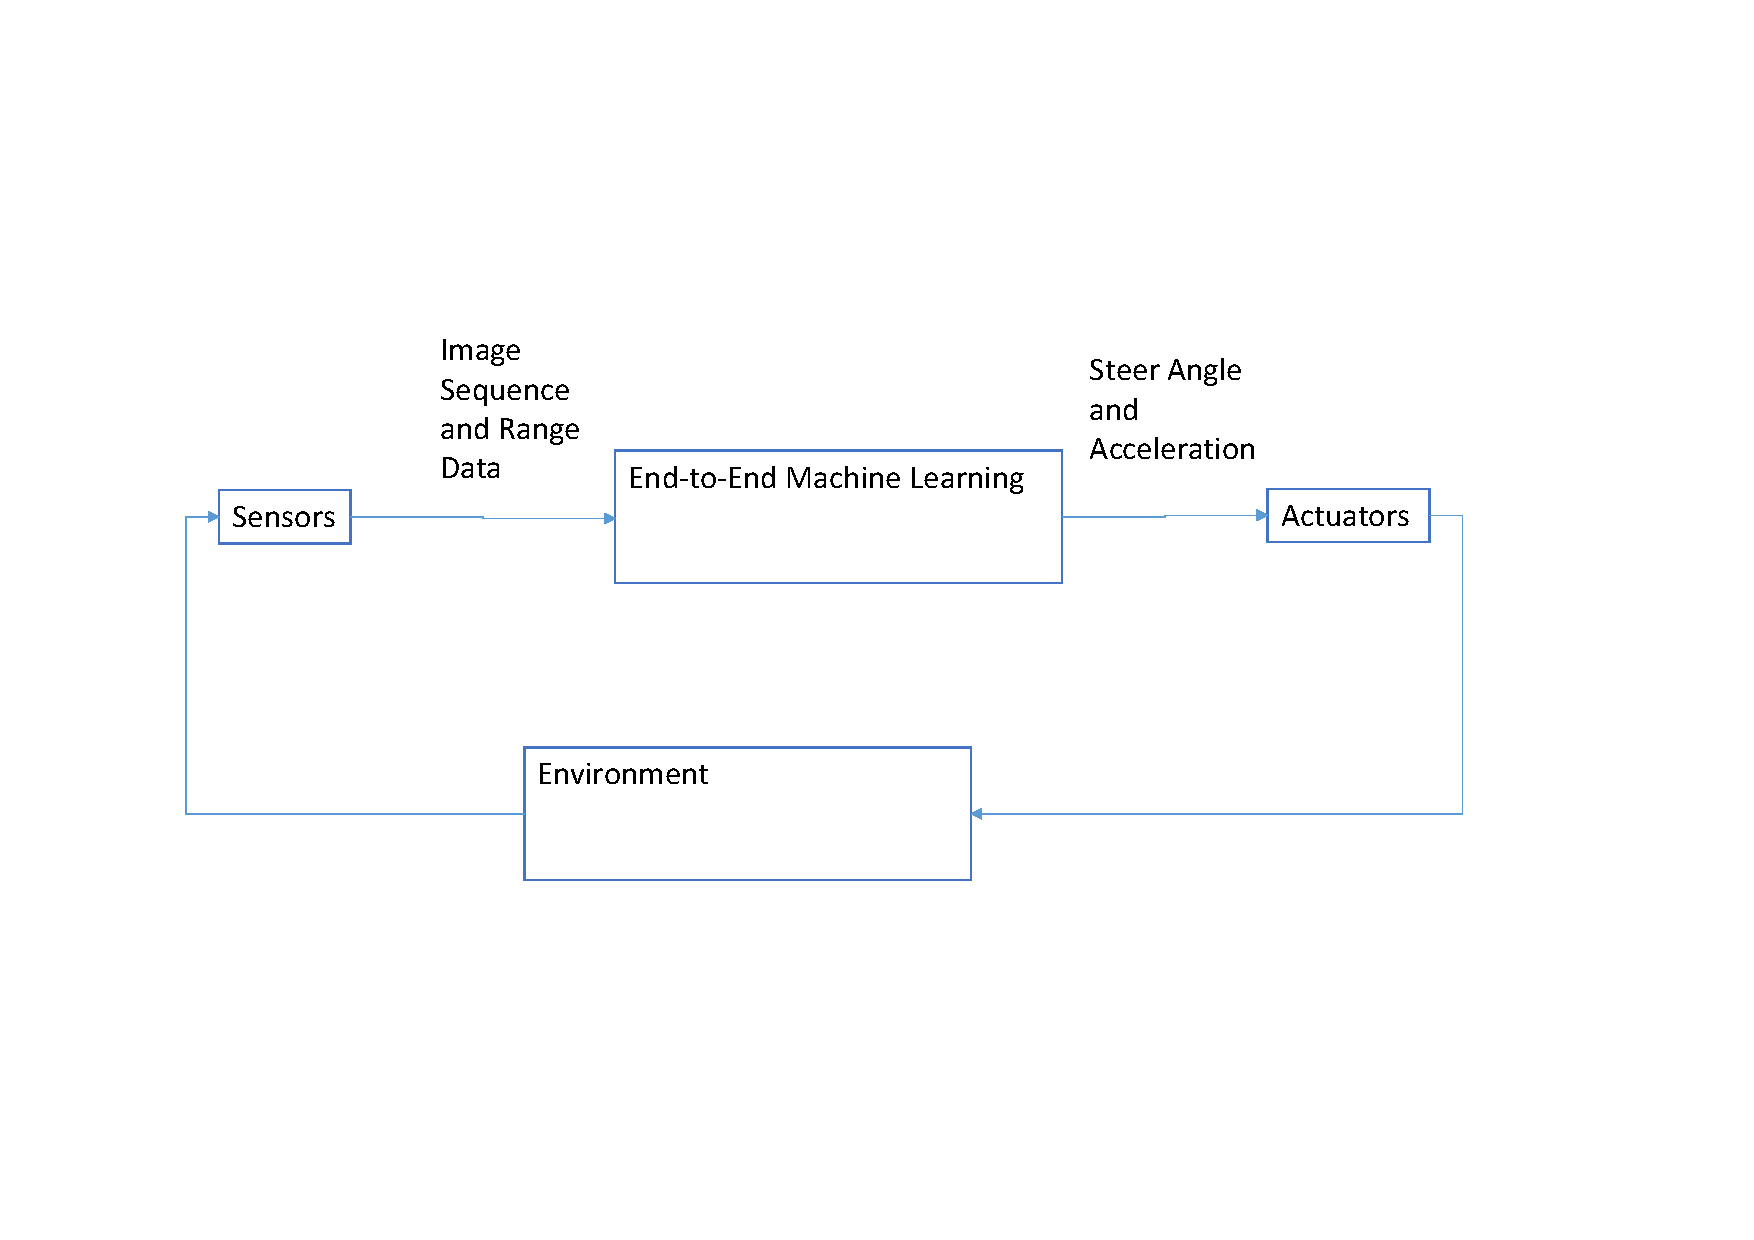
\includegraphics[width=\columnwidth, angle=-0]{EndToEndFlowChart}
	\caption{Logical flow of end-to-end planning}
	\label{fig:endtoend_flow}
  \end{center}
\end{figure}
\begin{figure}[ht]
  \begin{center}
	\includegraphics[width=\columnwidth, angle=-0]{BehaviourAwareFlowChart}
	\caption{Logical flow of interactive behaviour aware planning}
	\label{fig:behaviour_aware_flow}
  \end{center}
\end{figure}

Outcomes can be improved by combining behaviour choice with the motion planner, evaluating different behaviour options to choose the best. For multi-vehicle situations this can lead to interesting behaviour as some model of other vehicles decisions is needed in order to evaluate possible control actions. This could be obtained by inter-vehicle communication or traffic rules based and behavioural models of human traffic participants. At this stage, bringing in multiple participants is also out of scope, but the motion planning component may be useful to inform the type of plans which it is possible to exchange by inter-vehicle communication. Understanding the detail available in a single vehicle's trajectory plan determines the information it can share and also the way it can adapt to the plans of others.

An interesting recent addition to the list of architectures, end-to-end planning \ref{fig:endtoend_flow} eschews traditional distinctions such as perception from planning to instead train an artificial neural network (ANN) on image data from example test drives, so they are able to produce suitable steering commands based on the current video scene in \cite{Chi2017}. To get good results it was necessary to manipulate the training data by creating duplicate runs with a perspective offset, and a larger steering angle to correct the position. Otherwise there were not enough instances of large steering corrections in the data for a basic proportional controller to be learned which steered more vigorously the further it got from the road centre. Given the algorithm used to manipulate the data fully defined the steering behaviour it is hard to see the benefit of using machine learning in this case. It may be more appropriate to use the ANN to provide the behaviour choice and not the closed loop control, similar to \cite{You2019} where the ANN outputs five states - maintain, accelerate, decelerate, turn-left, turn-right, and operates on a simplified model of the traffic detected based on a grid. The actual actuator control - steering angles and acceleration can be completed separately. This should reduce training time by reducing the complexity of the ANN (fewer layers and fewer outputs) and also reducing the amount of noise as the environment representation is quite clean, reducing the chance of over-fitting. ANN based architectures are a useful complement to traditional methods and may be particularly appropriate when predicting the future actions.

Interactive behaviour aware planning is useful to concentrate on because they can utilize component from traditional planning where they are best suited such as feedback control and machine learning techniques where they are most effective, such as in behaviour choice. 

Hierarchical planning techniques are often based on sampling at some resolution from the configuration space, to create a discrete approximation to the problem which can be solved with graph techniques such as Dijkstra. These are able to guarantee resolution completeness, that up to the sampling resolution if a path exists it will be found.     

\section{Cut from JIRS Introduction}   

\subsection{Motivation for Path Adaptation}
Adaptive local path planning is important for the creation of robotic systems which can perform convincingly in variable environments. The particular environment of interest is one of bounded variation: there exists a fixed path which is preferable in most cases, but in certain circumstances it can be invalidated, for example by an obstacle. In this case it may still be possible for the robot to complete its task with a new path avoiding the obstacle, while keeping within a predefined tolerance of the original path to manage predictability. This paper will detail one approach for creating smooth paths for an autonomous vehicle with differential constraints on its motion, and compare two methods for adapting this path in response to an  obstacle detected by on-board sensors.   

\subsection{Paths and Trajectories}
\label{sec:traj_def}
A path is a continuous sequence of configurations. A trajectory is a continuous sequence of configurations each valid at a particular time. A path can always be extracted from a trajectory by discarding the temporal information, but an additional procedure is required to annotate a path with timing information usually based on a choice of speed profile. To ease computation both sequences may be obtained by dividing planning into two scales. 

\subsection{Division Based on Scale}
\label{sec:scale_division}
Large scale trajectory plans cover longer time periods so they can be called strategic plans by an analogy with business plans which cover longer time periods. At the other end of the spectrum small scale trajectory plans take place over shorter time periods so they might be called tactical plans.

Large scale path plans, having no timing information are usually called global plans. This is to distinguish them from local plans which only cover the immediate vicinity around the robot. 

There is no widely accepted scale threshold at which a plan is considered global, as different robots have different size operating domains. As a guide, a planner would be considered global if it is able to find a path between any two valid configurations in the entire domain of operation. A planner would be described as local if there is any limitation on the distance between the start and goal locations over which it can find a path if one exists. 

Global planning algorithms such as Probabilistic Roadmaps, dense random trees all require a local planner component. This component must be sufficient to connect nearby configurations (reach any final configuration) but does not have to account for obstacles. Obstacles are handled at the global layer. The local planner joins two nearby configurations by rejecting links which intersect with obstacles.  

\subsection{Division Based on Execution} 
There is an alternative definition of the local planner which is used by \cite{Walenta2017}, following the manual for ROS (Robot Operating System), a collection of software libraries (middleware) useful for creating robots \cite{rosbook2016}. Here a local planner is one which is able to generate a feasible path between any two adjacent nodes in the roadmap. It works in conjunction with a roadmap planner which efficiently produces large scale plans using Dijkstra or a related graph method. According to \cite{SicilianoKhatib2016} this approach is known Integration Planning, where the global reasoning is provided by a roadmap planner and augmented with a local trajectory planner which accounts for obstacles. This can comprise either a System for Tactical Planning which recomputes at high frequency a path to the target location or a System of Path Deformation which alters the reference path based on sensor data.

This is different from the definition of a local planner in Section \ref{sec:scale_division} where the local planner is an algorithm with limited capabilities, which is utilised by an obstacle avoiding global planner. To create a ROS *local* trajectory planner, an algorithm for global path planning of the type classified in Section \ref{sec:scale_division} would be needed, along with an appropriate speed profile. This is because a core function of the ROS local trajectory planner is obstacle avoidance.


\subsection{Problems with Shifted Curves and the PAN-Robots EU Project algorithm}
One promising technique for tactical planning is generating a set of alternatives with different offsets from the reference path and choosing the one satisfying obstacle constraints as in \cite{Chu2012}. This is a very convincing solution to the stated problem of path modification with limited variation. It is comparable to the method presented here as the form of the path is fixed but will always be suboptimal unless the number of alternatives is made extremely high.  

Shifted curves inevitably compromise solution quality by limiting the search space. This is one example of an approach based on sampling from the search space. More sampling based methods are reviewed in Section \ref{sec:sampling_based}.

\cite{Digani2014} uses an algorithmic method, which divides an avoidance manoeuvre into three stages and generates a simple cubic section for each: a lane change with an s-curve, passing the obstruction, and another lane change back onto the reference path. Collision checking is not actually addressed in detail, but described as a comparison of the free space 'size' with the size of the AGV. I am left with several questions, such as: What dimension is compared? Does it depend on the avoiding path and obstacle and AGV shape?    

>>>
%TODO: Consider IF these work summaries can be included in the Method section of the JIRS paper, rather than the introduction

%\section{Similar Work Summaries}
\subsection{Root Finding}
6. Root finding is used by \cite{Gim2017}, where a modified bisection method is used to find the roots of the lateral position error to a target final pose in $(\alpha, \delta)$ parameters space. By matching the curvature and heading at the end of the curve, a sequence of two or four clothoids is described by only the sharpness $\alpha$ and deflection $\delta$ of the first segment.
 
\subsection{Constructive Polylines}
7. An earlier geometric method from \cite{Henrie2007} is able to find the parameters for a CC-Path based on clothoids to join any two poses with zero curvature at the start and end. This requires that each pair of clothoids be symmetrical and end with zero curvature. The authors call this the ``generic turn'' procedure. This approach is developed further in \cite{Wilde2009} with a one dimensional search to find the least maximum sharpness. By the definition of sharpness as the rate of change of curvature with path length, this leads to the path which can be traversed at a given speed with the slowest steering rate. This should lead to smooth and easily drivable paths.

\subsection{Tactical Motion Planning}
%OR
8. The problem addressed in the current work is that of computing an optimal alternative path, given an obstruction which invalidates the reference path. It is important in an industrial environment where reference paths can be designed and are preferable to any seemingly convenient adaptive path for reasons of safety and predictability. The only reason a new path is needed is in the case the reference is invalid, due to an unexpected obstacle. This problem will not result in a complex obstacle maze, and if it does it is undesirable for a robot to navigate it. These are industrial robots, not explorers, but if there is an obvious and safe workaround to a problem they should be able to detect it and plan accordingly. If there is no clear solution, it is always better to alert operators and wait for assistance, than to forge into the unknown and risk creating unsafe and unpredictable situations.  

\subsection{Sampling Based Planning Techniques}
\label{sec:sampling_based}
\subsection{Introduction}
Geometric path planning or the piano mover's problem consists of finding a sequence of configurations between an origin and a destination within a field of obstacles. The problem is known to be PSPACE hard, that is to require at least a polynomial amount of memory to solve. It has been a topic of active research in robotics and animation for the last several decades and many practical  solutions have been developed, especially for the case of a two dimensional workspace with polynomial obstacles. An overview is given in Handbook of Robotics, Part A: Robotic Foundations - Motion Planning \cite{SicilianoKhatib2016}. 

\begin{figure}
\label{fig:problem_statement}
Given:
\begin{enumerate}
\item A workspace $\mathbf{W}$ is either in $R^2$ or $R^3$
\item An obstacle region $\mathbf{O}$
\item A robot defined in $\mathbf{W}$ consisting of one or more rigid bodies
\item A configuration space $\mathbf{C}$ comprising $\mathbf{C_{obs}}$ and $\mathbf{C_{free}}$
\item An initial configuration $q_I \in \mathbf{C_{free}}$
\item A goal configuration $q_G \in \mathbf{C_{free}}$
\end{enumerate}
Compute a continuous path $\tau : [ 0, 1] \rightarrow C_{free}$ such that $\tau(0)=\mathbf{q_I}$ and $\tau(1) = \mathbf{q_G}$
\caption{The piano mover's problem - geometric path planning.\cite{SicilianoKhatib2016}}
\end{figure}
Typically approaches make some approximation to make the problem tractable, at the cost of some aspect of global optimality of the solution. Approaches may be divided roughly into Mathematical Programming based and Sampling Methods, although there are others such as Potential Field methods and many combinations.

Sampling methods for motion planning can be divided into deterministic and randomized sampling. Deterministic samplers subdivide state space into a uniform lattice such as a grid or a more exotic symmetrical structure designed to span the search space effectively. Randomized sampling methods fall into two main categories: Rapidly Exploring Trees (RRTs) \cite{LaValle2000} and Probabilistic Roadmaps (PRM). Probabilistic roadmaps are typically used for static environments, where it is advantageous to make multiple queries on the same roadmap, for a robot performing different taks within the same environment. This is because it is time consuming to produce a new roadmap but quick to make additional queries on it. RRTs are more useful when the environment is changing rapidly such as a robot exploring new areas. The tree is quick to construct but there is little advantage to making subsequent queries.


\subsection{State Lattice Planners}
\label{sec:state_lattice_planners}
Sampling from the state space in a regular lattice to create a graph for efficient searching is one of the first practical approaches to path planning for mobile robots. This is because the computational complexity was low enough for real-time systems provided certain assumptions held. Typically the lattice took the form of a regular grid, either four connected or eight connected by straight lines. Each node represented the x-y state of a holonomic robot, able to move in any workspace direction freely. The holonomicity assumption allows many interesting path finding behaviours to be studied, but typically does not hold for practical systems like cars or fork lift trucks with Ackerman steering which are subject to differential constraints.

\begin{figure}
\centering
\def\svgwidth{1.0\columnwidth}
\input{Chapters/Chapter1/Chapter1Figs/hierarchy.pdf_tex}
%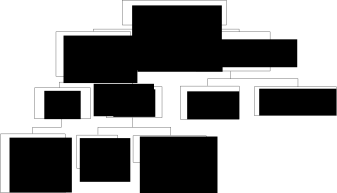
\includegraphics[width=\columnwidth, angle=-0]{hierarchy}
\caption{Hierarchy of planning approaches. See 'Handbook of Robotics, Part A: Robotic Foundations - Motion Planning' \cite{SicilianoKhatib2016} for more details.}
\end{figure}

\subsubsection{Smoothing}
One way of incorporating differential constraints into the lattice planning approach is to fit a smooth curve which respects the constraints such as a cubic spline as closely as possible to use nodes returned by the planner. The difficulty here is that the smooth curve does not exactly follow the edges in the graph which were used to calculate the route cost and check for obstacle intersection. If the cost of the smooth path is different to that of the approximation used in the lattice, any optimality guarantees provided by the planning method such as Dikstras algorithm are compromised. Worse, the smooth path must be checked against the obstacle map for collisions, and it is not clear how the path should best be modified if any collisions are detected. For an example of smoothing with clothoid curves see \cite{Lundberg2017} \cite{Walton2005}.

\subsubsection{Differential Constraints}
It is possible to carefully construct a lattice which captures differential constraints as detailed by Pivtoraiko et al \cite{Pivtoraiko2009}.The trick is calculating the control inputs required to join a set of vertices which span state space (inverse kinematics) or sampling from the control space in order to generate a set of vertices (forward kinematics). Both methods have complications, for example the shape of the lattice must be known ahead of time to be reachable with a simple set of primitives for the inverse method. For the forward method the difficulty is in the choice of interval in control space that leads to complete and uniform coverage of state space. These difficulties are resolved for one example configuration in \cite{Pivtoraiko2009} with 16 discrete headings, 8 levels of curvature and a total of 192 controls. The balance to be struck in the choice of resolution is that higher resolutions lead to a higher branching factor, increasing the memory required to represent a given area, but lower resolutions will give suboptimal paths. Imagine following a straight wall which does not align with one of the 16 cardinal directions in the lattice, but halfway between. The planner with return an optimal path which alternates between the two closest cardinal directions, rather than a straight line aligned with the wall. With a back of the envelope calculation, increasing the resolution to 10mrad to minimize artefacts increases the number of nodes required per square metre to exceed the number of atoms in the known universe. This trade off is the biggest obstacle to the use of lattice planners for general path planners and led to the development of randomized planners, which can give satisfactory uniformity and coverage of high dimensional state space without the direct link between the branching factor and the resolution when constructing a lattice.   

\subsection{Probabilistic Roadmaps}
Probabilistic Roadmaps are an example of a multiple-query sampling based planner. They are probabilistic in the sense they sample randomly from $\mathbf{W}$ to build up a connectivity graph - the roadmap. They do not inherently cope with uncertainty in the obstacle field.
One important component is a local planner, which is able to generate a path between two nearby configurations and test if it intersects with any obstacles. The algorithm proceeds by testing each sample by creating a local path from the nearest point on the existing tree, and only adding the new point to the graph is the path is obstacle free. Depending on the local planner it is possible to incorporate smooth paths respecting vehicle dynamic limits, but other methods are more appropriate in cases where the obstacle field is dynamic because the simplifying assumption making roadmaps so fast is that of a static environment. 
Another important component is the graph method used to select the shortest path such as Dijkstra which is used to find the shortest path once the roadmap is constructed. There also must be some heuristic guiding the selection of new points.

The distinction between PRMs and lattice planners is only in the mechanism by which samples are drawn from state space to construct the roadmap \cite{SicilianoKhatib2016}. They are both Roadmap planners. Either a repeating pattern or lattice is overlaid or states are selected randomly within an area of interest and discarded if they are not reachable according to the obstacle map and the local planner. This is based on the idea that randiom samples of high enough density will provide unbiased and complete coverage of the space. Particularly in the limit as the number of samples tends to infinity, a PRM may be 'probabilistically complete' so that as the number of samples tends to infinity the probability of finding a solution if one exists tends to one.

The modifications to both types of Roadmap planners which deal with a changing environment and differential constraints on motion are very similar. Differential constraints can be incorporated into the local planner as described in \ref{sec:state_lattice_planners}, alththough there are fewer constraints on PRM as there is no need to use kinmatics to ensure the samples form a regular lattice. 

\subsubsection{Uncertainty}
Both types of roadmap planner are useful for dealing with uncertain representations of the world where the environment is represented as an occupancy grid, a grid of values covering the space, each value representing the occupancy probability of that cell. The best path can be found directly from this representation by minimising the sum of occupancy probability of every cell traversed by the path. This may be more useful than the 'hard constraints' offered by optimization methods, because although the solution will not violate the constraints, the constraints themselves are constructed by throwing away information about the uncertainty of the environment to create a binary representation where every position in space is either inside or outside polygonal obstacles \cite{Pivtoraiko2009}.     

\subsection{Rapidly Exploring  Random Trees}
Rapidly Exploring Random Trees are an example of a single query planner introduced by LaValle and Kuffner \cite{LaValle2000}. Most simply, a tree is constructed by sampling from state space close to an existing node in the tree. A local planner is used to generate a trajectory from the existing node to the new sample avoiding obstacle regions if one exists. If an obstacle free trajectory is found, a new node is added at the sample state with an edge from the existing node. Nearby nodes in the tree should also be checked and connected with edges if possible. 

Starting with the initial position and the goal position, this process is repeated until sufficient coverage of the state space is obtained. When a new sample is reachable from both trees, origin and destination must be connected and a graph method such as Dijkstra can be used to identify the vertices through the graph which make up the shortest path between them. The tree growing phase of the algorithm can be terminated at this point but it may be possible to improve the quality of the solution by adding more reachable states to the connected graph in case  a better solution can be found.  

\section{Automated Intersection Management Literature Review} 
Studies on the theoretical capacity of signalized intersections and roundabouts with an equivalent footprint indicate that in most cases, if there are few approach lanes small roundabouts will tend to have higher capacity. If there are many approach lanes signals tend to be more effective, unless the traffic on different approaches is extremely unequal \cite{Jian-an2001}. 

A systematic procedure computing the conflict points in an intersection is given in \cite{Lu2013}. Roundabouts tend to have a large number of merging and diverging conflicts, but fewer or none of the crossing and head-on conflicts which lead to the most serious collisions due to high relative speeds.

Intersection control often addresses crossing conflicts by separating vehicles in time, while they all take the shortest path straight through the intersection in the same way as if it was signal controlled. There are a wide range of optimal and heuristic approaches to solve for the speed profile, both decentralized and centralized, a good review is given in \cite{Rios-Torres2017}. Many studies have looked at how to incorporate a proportion of human controlled vehicles which are not able to communicate their intention. One way of doing this is using traffic signals which only apply to human drivers \cite{Zhao2019}. The downside is that the nature of the intersection must remain similar to a traffic-light controlled one if non-communicating participants are going to be controlled by lights.

Recently a number of studies have extended intersection coordination of Connected and Autonomous Vehicles (CAVs) to the resolve the type of merging of diverging conflicts which occur and roundabouts. These are reviewed in \cite{Rios-Torres2017}. A centralized solution with an intersection manager minimizing delay and energy consumption is described in \cite{Zhao2018}. This shows that a high proportion of vehicles need to be communicating for significant benefits to be realized. 

A decentralized approach based on intent communication by way of virtual vehicles, can also be applied to roundabouts. In \cite{Debada2016}, reactive heuristics are shown to lead to poor performance compared to a model predictive control approach. The virtual vehicle concept allows common lane based heuristics such as car following to be extended to resolve conflicts in  \cite{Debada2018}. Another work investigating virtual lanes is \cite{Xu2018}. Here a conflict graph is used to assign approaching vehicles to appropriate virtual lanes and a distributed controller is presented to stabilize the platoon.

Another approach presented in \cite{Liu2018} is a decentralized solution to the global problem of minimizing the delay. Proofs of completeness and optimality of the aggregate problem are given, making this technique very impressive. It is not shown to be applicable to roundabouts in any of the numerical examples, although the incorporation of optimal trajectory planning by the low level controller to execute merging makes it a good example of the combination of path planning and intersection management. Collision constraints are based on a conflict zone rather than conflict points as in \cite{Levin2017}. The location of the conflict points is fixed by the fixed paths between the entry and exit lanes of the junction. The space inefficiency of the zone representation for multiple lanes is addressed by using multiple zones, one for each pair of lanes. The use of simultaneous path optimization might be expected to increase computational complexity and thereby reduce the number of vehicles with can be routed, however an attached video showing many vehicles interacting for about 10 minutes seems to refute this. It seem the ordering problem is resolved in a decentralized way based on game theory and the game `Chicken.' Using game theory to resolve the ordering problem may give this approach an edge over the mixed integer optimization used in \cite{Levin2017}, in terms of how many vehicles they can control before running into execution time limits. It is a little surprising that the game would always produce the optimal ordering given the motion model used by each AGV. The consensus mechanism will be important here. Questions remain about the possibility of AGVs disagreeing about the order they calculate from the communicated position and speed data. 

A similar method which solves the ordering ordering problem sequentially, followed by individual optimization of the approach speed along fixed paths is described in \cite{DeCampos2017}. This method claims only local (per-vehicle) optimality for the speed choice sub problem, and makes it clear the crossing order at convergence will be suboptimal, and depends strongly on the decision order. The sub problem is posed as a Linear Quadratic Regulator, commonly seen in optimal control problems. In general terms, those early in the decision order will deviate from the plans less. This is more of a problem when vehicles are not uniform, as to reduce energy consumption a late arriving lorry should deviate as little as possible. A heuristic is given for the decision order based on the time to conflict arrival.

The use of optimal control in \cite{DeCampos2017} is shared with many earlier works regarding coordination of Unmanned Arial Vehicles, many of which relax the assumption of static paths. In this way \cite{Schouwenaars2004} addressed the full multi-vehicle motion planning problem for small numbers of aircraft with simple dynamics. The craft were assumed to be differentially flat: that is, able to actuate in any of the workspace degrees of freedom independently, like a quadrotor. They were represented using bounding rectangles, leading to a slightly conservative mixed integer problem. The integer variables are used to choose which constraints are active. This might seem excessive when representing static obstacles, however when the constraints arise from other moving vehicles, the integer variables are a natural way to represent the passing-order problem. The scaling to larger numbers of vehicles is a particular challenge, due to the combinatorial explosion of possibilities.

An alternative approach to the coordination of differentially flat aircraft which uses a sequential solution of per-vehicle receding horizon sub problems to approximate the global solution is given in \cite{Keviczky2008}. An earlier theoretical treatment based on iterative bargaining with soft collision constraints is given by \cite{Inalhan2002}. The parameters are real numbers, and the constraints linear while the cost is quadratic. It may converge to an infeasible solution given a particular minimum safety distance even from a valid set of starting positions and speeds, and the suggested solution is to reduce the threshold until it becomes feasible.  

More recently, solutions based on Distributed Model Predictive (DMPC) control have been developed. In \cite{Dai2017}, per-vehicle optimizations runs simultaneously to reduce execution time. This ensures recursive feasibility and closed loop stability. Another DMPC approach is given by \cite{Luis2018}. This scales up to 25 vehicles in real time. the quadrotors concerned are all identical and differentially flat. For an under-actuated system like an AGV, some of the simplifications may no longer be possible.
 
%=== Chapter Two ===
\chapter{Dynamic Platooning for Automated Guided Vehicles (AGV)}



\section{Introduction}
AGV typically have their motion restricted to a roadmap connecting pick and drop locations \cite{Cardarelli2017}. This reduces the search space to make conflict free routing of multiple vehicles between different origins and destinations feasible. \cite{Digani2015} proposes a two level decomposition of the problem with the detailed roadmap at the bottom and a higher level abstraction of zones around each intersection above. The conflict avoidance is handled with local information within each zone. The routing decisions are made at high level, utilizing a traffic model where each intersection has a fixed capacity (number of vehicles). 
 
%\section{INTRODUCTION}
Coordinated conflict-free motion of a number of mobile robots in order to complete a material transfer task is important in the operation of fleets of AGV (Autonomous Guided Vehicles) used in flexible manufacturing and automated warehouses \cite{Vis2006} and \cite{Dotoli2019}. A crucial sub-problem is conflict resolution between multiple AGVs, without control of task assignment or scheduling.

It is shown, in \cite{Digani2019}, that platooning provides superior throughput to the earlier reservation based systems, and that if a solution exists it is optimal, but not that a solution exists on all roadmaps. More importantly a set of conditions which must hold for a solution to exist, is not given. The consensus algorithm in \cite{Tadano2019} also shows improved throughput in concert with a scheduling approach, but does not prove convergence. 
An example of a resolution complete algorithm based on spatial reservation is \cite{Draganjac2020}. Neither per-intersection optimal platooning nor per-vehicle consensus have been proven complete. The lack of guarantees is an important limitation of platooning methods for collision avoidance. The research gap identified is the lack of investigation into the range of motion conflict situations that can be resolved with platooning methods.

\section{Literature Review}
AGV motion coordination can be posed as a variation of the Multiple Vehicle Routing Problem with the addition of challenging spatio-temporal constraints preventing collisions between each vehicle, as well as the usual timing and capacity constraints \cite{Miyamoto2016}. In \cite{Li2017}, solutions are classified into centralized, decentralized and decoupled approaches. Each approach may be either optimal or heuristic based on whether or not they find the global minimum of some objective function. 

It is also possible to classify approaches based on the limitations they place on the state space of each AGV. Most practical methods incorporate both obstacle avoidance constraints and differential motion constraints into some sort of roadmap. This is often a graph with vertices at key points in the reachable state space, connected by edges representing feasible motion between them. The effect of increasing resolution on path quality (measured by reduction in the length of the shortest path) and computation time are studied in \cite{VanDenBerg2005}. 

Interest in centralized methods which plan in the full state space all of the vehicles was renewed by the development of effective numerical tools for operations research able to solve large combinatorial problems to optimality. Notably \cite{Richards2002} found trajectories for aircraft using a linear approximation to the dynamics and obstacle constraints, allowing the use of Mixed Integer Linear Programming. The contribution of \cite{Li2017} is to describe a new centralized, optimal method which scales well, finding a solution to the nonlinear-program for 10 vehicles in just a few seconds using an interior point method. However, size of the combined state space explodes as more vehicles are included so centralized methods are difficult to scale up to large numbers of vehicles.

Many types of decoupled methods have been developed because breaking the problem down into sub-problems is one way to reduce computation time for practical applications. Early methods of this type were based on timed petri nets \cite{Dotoli2004} and agent based models \cite{Singh2002}. Decoupled methods may sacrifice completeness (that a solution is found if one exists) in exchange for reduced average run-time. In \cite{Sanchez2002}, this was shown to cause practical difficulties in the spot-welding task studied. Spot welding requires close formation control of six vehicles, and the decoupled method frequently failed to find a solution. In \cite{Peasgood2008}, decoupled planning (incomplete) is compared with a new multi-phase heuristic, which is complete, for 50 robots on a tunnel map and 150 on an outdoor map. Decoupled planning was consistently faster in execution and produced shorter paths for lower vehicle density however it failed to find any valid paths at all for high vehicle density (25 or more robots in tunnels and 75 or more outdoors). The multi-phase heuristic, being complete, found a solution in every test case. 

More recently, \cite{Yu2013} addressed the lack of optimality in decoupled methods operating on graphs. Optimal conflict-free motion is posed as a large Integer Linear Program. Resolution complete general purpose algorithms are used to solve it for 150 robots in just over 10 seconds. The lattice/graph construction has recently been developed further to ensure kinematic constraints are met and improve coverage of state space around obstacles \cite{Yu2018}. In \cite{Miyamoto2016}, the combined problem of DCFVRP (Dispatch and Conflict-Free Vehicle Routing Problem) for flexible manufacturing is formulated as an integer program and two different decoupled algorithms are presented to solve it: local search and random search. Neither of the proposed algorithms is complete but local search found more valid solutions in the 10 random examples tested, all involving three vehicles.

Decentralized control is another option to decompose large scale problems which take too long to solve centrally \cite{Bakule2008}. Although limiting the information available to each decision maker can make reasoning about collective behavior more difficult, various attempts to decentralize conflict-free routing have been made. 
In the field of conflict free routing for mobile robots, \cite{Draganjac2016} presents a solution which generates a graph representation of the free space - effectively a roadmap - with the property of `collision-avoidability.' This means that every node on the critical path must be at most one move away from a node that does not obstruct the critical path. The critical path is defined as the union of all the shortest paths between pick/drop locations in the roadmap. During decentralized planning, AGVs attempt to reserve `private zones' consisting of the node on the critical path along with all adjacent collision avoidance nodes. Each AGV has an identical roadmap, plans the shortest path to its own goal and negotiates with those nearby based on a numeric priority to reserve the nodes in its own path. An AGV requests those in its path move to their collision avoidance node, and those with a lower priority will do so. Proof is given of correctness, that deadlocks are avoided, but throughput is sub-optimal with low priority vehicles frequently forced to stop and wait. %Another decentralized method based on sequential reservations is given by \cite{Walenta2017}, without the concept of 'private zones' to avoid deadlocks however. 
An alternative decentralized solution, based on a roadmap with two levels of detail is summarized in \cite{Sabattini2018}. Conflict-free routing primarily takes place at the most detailed level, based on prioritized roadmap reservation with local negotiation to guarantee correctness \cite{Digani2014}.  In \cite{Digani2019}, the speed of the approaching AGV is optimized at each intersection in a similar way to centralized intersection platooning. The result is higher throughput as time consuming negotiation is avoided in most cases.      

Congestion effects are represented by link performance functions in the approximate level graph. Intersections have a generalized cost which increases exponentially up to a fixed capacity which identified by parameter tuning, An optimal task scheduling approach based on the Hungarian Algorithm is used to solve the full DCFVRP in \cite{Sabattini2015a} and \cite{Sabattini2018}. Traffic delays are a type of emergent behaviour and modelling is challenging even in a completely automated system. This is the contribution of \cite{Street2020} which introduces the PRT (Probabilistic Reservation Table) to summarize the plans of robots including uncertainty so it can be in task scheduling. This approach is compared with a reservation based centralized planner as a baseline, in a simulation with 5 robots using a low level motion controller from ROS (Robot Operating System) which often fails at when two robots plan interfering paths. Congestion aware planning leads to fewer failures of the low level controller than independent planning but more than centralized planning. A more convincing comparison would be with a congestion aware planner using a deterministic congestion model instead of the PRT, but this is not reported.

Intersection control, based on platooning, is a concept developed for the operation of anticipated CARVs (Connected and Autonomous Road Vehicles). A recent review of approaches for intersection and merging coordination is given in \cite{Rios-Torres2017}. Centralized optimization approaches improve on early ideas like First-Come-First-Served spatial reservation from \cite{Dresner2008} by minimizing fuel consumption, but the rapid increase in state space with larger numbers of vehicles will need to be addressed before large scale adoption. The communication channel connecting every vehicle with the central controller introduces a single point of failure, the reliability effect of which is difficult to evaluate in existing simulations. Moreover there are few CARVs available making a practical experiment unfeasible in most cases. Attempting to address these limitations are decentralized methods such as fuzzy-logic, virtual vehicle platooning and invariant set approaches. Notably the conditions for solutions to exist which minimize energy consumption are given in \cite{Malikopoulos2018}.

Recently \cite{Tadano2019} described an approach to the DCFVRP for flexible manufacturing based on dynamic platooning with vehicle-to-everything messaging and consensus speed control, resulting in a decentralized heuristic solution with some additional rules to ensure correct behavior and avoid deadlocks by adding a reservation protocol for some parts of the roadmap. This was combined with feedback from the queue length at different workstations in a traffic management heuristic. Simulation results show an impressive improvement compared to the first-come-first-served scheduling approach meant to represent industry standard practice.   

A promising approach for intersection control applied to AGV is given in \cite{Digani2019}. As the paths are not modified, only the speed adjusted deadlocks are proved impossible. However, a backup system based on negotiation is still required because the problem is non-convex suggesting a feasible solution may not be found in time for certain roadmap and traffic combinations. The consensus based platooning method for local collision avoidance used in \cite{Tadano2019} is unusual in the AGV domain. That work makes no claims about completeness, but does consider the trivial consensus where all vehicles stop in a deadlock. In \cite{Zhang2018}, a recent system for conflict avoidance based on time headway is shown to significantly reduce intersection crossing time and allow more vehicles to operate in the same floor-space compared to a traditional reservation based strategy. Of these different approaches to platooning for AGV coordination, the quadratic constraints of \cite{Digani2019} are the closest to acheiving the certainty the would be required to build a distributed coordination scheme.
%\section{METHODOLOGY}
%
%With existing methods, a backup system is needed to prevent collisions in exceptional cases, as there is no proof of completeness of the main algorithm. A proof might be possible placing certain conditions on the traffic flow or the roadmap layout, but this is left for further work. Instead we focus on simulation to identify situations where convergence is more or less reliable. This will help to identify sites where the potrential throughput benefiits can be realized because the slower fallback option will be needed less often. It may also highlight situations in which current methods frequently fail, and help to inform modified algorithms to address these cases.  

%\begin{figure}[htbp]
%\centerline{\includegraphics[width=1.0\linewidth]{single-track-layout.png}}
%\caption{Single-track grid layout}
%\label{fig:single-track-layout}
%\end{figure}
%%[htbp]
%%\scalebox{0.5}[heightscale]{}
%%\resizebox{1.0\linewidth}{1.0\linewidth} %only for \include{graphics}
%%\centerline{\includegraphics[width=1.0\linewidth]{single-track-layout.png}}
%\begin{figure}[htbp]
%\centerline{\includegraphics[width=1.0\linewidth]{highway-layout.png}}
%\caption{Highway grid layout.}
%\label{fig:highway-layout}
%\end{figure}

%To test the success rate in finding a solution from a variety of initial conditions, we assume all AMR follow their planned trajectory exactly and look for cases where the platooning algorithm did not converge before the intersection, leading to a collision. The trajectory of each AMR must be tracked over time at a relatively high frequency, such as 10hz. Circular bodies of fixed radius can be assumed to make collision checking straightforward. Lateral dynamics can be neglected by assuming the path following controller is successful and tracks the path exactly.  Second order dynamics enable comparison of energy consumption resulting from platooning. Deadlocks and Live-locks can both be checked based on a time threshold for a vehicle to complete a job e.g. the transfer time plus the length of time it would take a vehicle to traverse the entire roadmap. If either is exceeded the simulation state should be recorded for further analysis. 
%
%In order to do this a number of realistic roadmaps are required, along with sensible parameters for vehicle size, acceleration and top speed. These can be estimated based on the literature such as \cite{Boysen2019} and \cite{Dotoli2019}. Important classes of roadmap which may be representative include grids, one-way aisles and two-way aisles.  such as those in Figures \ref{fig:single-track-layout} and \ref{fig:highway-layout}. 


%Conflict avoidance is only one part of the DVFVRP problem, the job assignment method has a profound affect on the frequency and complexity of the motion conflicts which need to be resolved. For this reason it is important to track genuine transfer jobs, assigned to a fixed number of `physical' vehicles (they do not appear and disappear at convenient times and move only according to a second order dynamic model). There is a separate question of which job scheduling algorithm and associated traffic model is best suited to each conflict-resolution method which we will not address here. For simplicity of exposition and ease of reproduction we will use a nearest-first-come-first-served scheduling approach to create traffic for both conflict-resolution methods. This is sufficient that the  number of transfer tasks completed can be tracked in a simulation of `physical' vehicles. Improvement of productivity using a traffic model and the Hungarian algorithm (e.g. \cite{Sabattini2015a}) is left for further work. We know of no reason it would benefit one method in particular.
\section{Simulation}

Platooning with speed choice by a centralized controller was implemented with a vehicle to intersection messaging scheme. The full site is divided into zones, each one containing a single intersection. Each AGV in the fleet has a copy of the roadmap which is  static. The fleet controller interfaces with the warehouse management system to get the next material transfer job, consisting of a pick location and a drop location. All jobs are assumed to be of unit size and each AGV has a capacity of one unit. With these assumptions, a straightforward policy is to assign the next job to the AGV nearest to the pick location - first-come-first-served scheduling. When an AGV receives a new job, it finds the shortest path through the roadmap using the Floyd-Warshall algorithm \cite{Djojo2013}. Next it must send its planned path to the intersection controller for the zone it currently occupies. The intersection controller stores the plan and current position of every AGV approaching the conflict point of the intersection. Every time it receives a new plan it must recalculate the approach speed for every approaching AGV to minimize total travel time without collision. This will happen every time an AGV enters the zone from somewhere else, or an AGV within the zone is assigned a new job.

%\begin{figure}[ht]
%\centering
%\includegraphics[width=\linewidth]{intersection_layout_trim}
%\caption{Intersection layout shown in SUMO NETEDIT tool \cite{dlr2016}}
%\label{fig:layout}
%\end{figure}
\begin{figure}[ht]
\centering
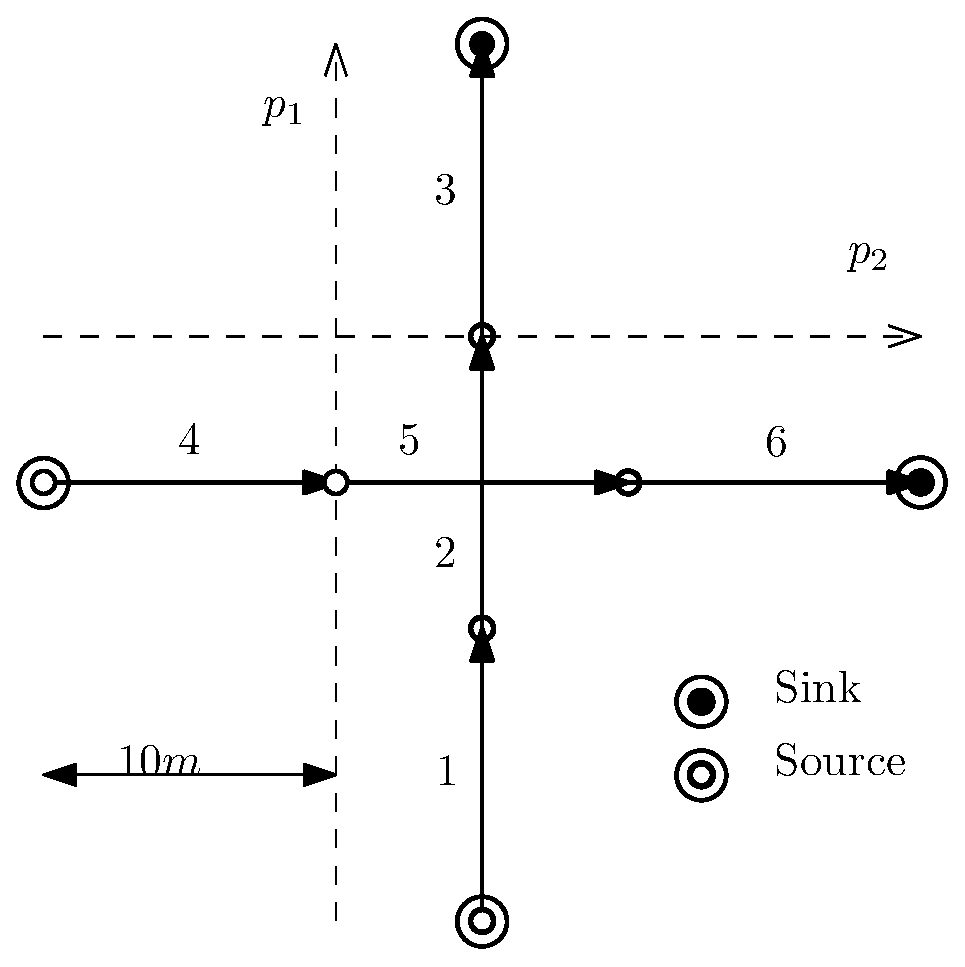
\includegraphics[width=0.9\linewidth]{intersection_topo}
\caption{Intersection layout with two conflicting routes.}
\label{fig:layout}
\end{figure}

The intersection controller was implemented based on \cite{Digani2019}. The surrounding lanes are first discretized into segments. The intersection shown in Figure \ref{fig:layout} is divided into six segments, each of length 10 meters. The critical segments are the two that cross in the center. There are two routes defined, one starting on the left and traveling to the right and the other starting at the bottom and traveling up. One AGV takes route 1 and the other takes route 2. If they both travel at maximum speed they will collide in the center.

The dynamic model for each AGV assumes they are able to exactly follow the path, and attempt to reach the target speed for each segment subject to a limited rate of acceleration of $a m/s^2$. 

\begin{figure}[ht]
\centering
\includegraphics[width=0.9\linewidth]{SystemSetup3.pdf}
\caption{Messages exchanged by participants approaching intersection.}
\label{fig:system_setup}
\end{figure}

The ApproachPlan message sent by the AGV contains a sequence of segments which it intends to traverse, along with its current distance along the first one.  The flow of messages is shown in Figure \ref{fig:system_setup}. The SpeedList sent by the intersection controller contains the optimal speed for every segment in the plan. The speeds can be found with the nonlinear program in Equation \ref{eq:qp_speeds}. 

\subsection{Motor Dynamic and Electrical Model}
The simulated AGV are based on a small payload 100kg total mass, with a maximum speed of 10m/s and peak acceleration of 5m/s$^2$, allowing them to stop safely within 10 metres. The intersection controllers use a constant acceleration model to calculate the time and space deadlines they pass to the AGV. To make the simulation test worthwhile a simulation model with slightly more complexity was used to evaluate the performance.


The brushless DC electric motor used in \cite{Racewicz2018} has suitable properties to propel a 100kg battery powered vehicle. A DC motor can be modelled by the steady state equivalent circuit shown in Figure \ref{fig:dc_circuit} which is well known, for example see \cite{Hughes2008}. 

\begin{figure}[ht]
	\centering
	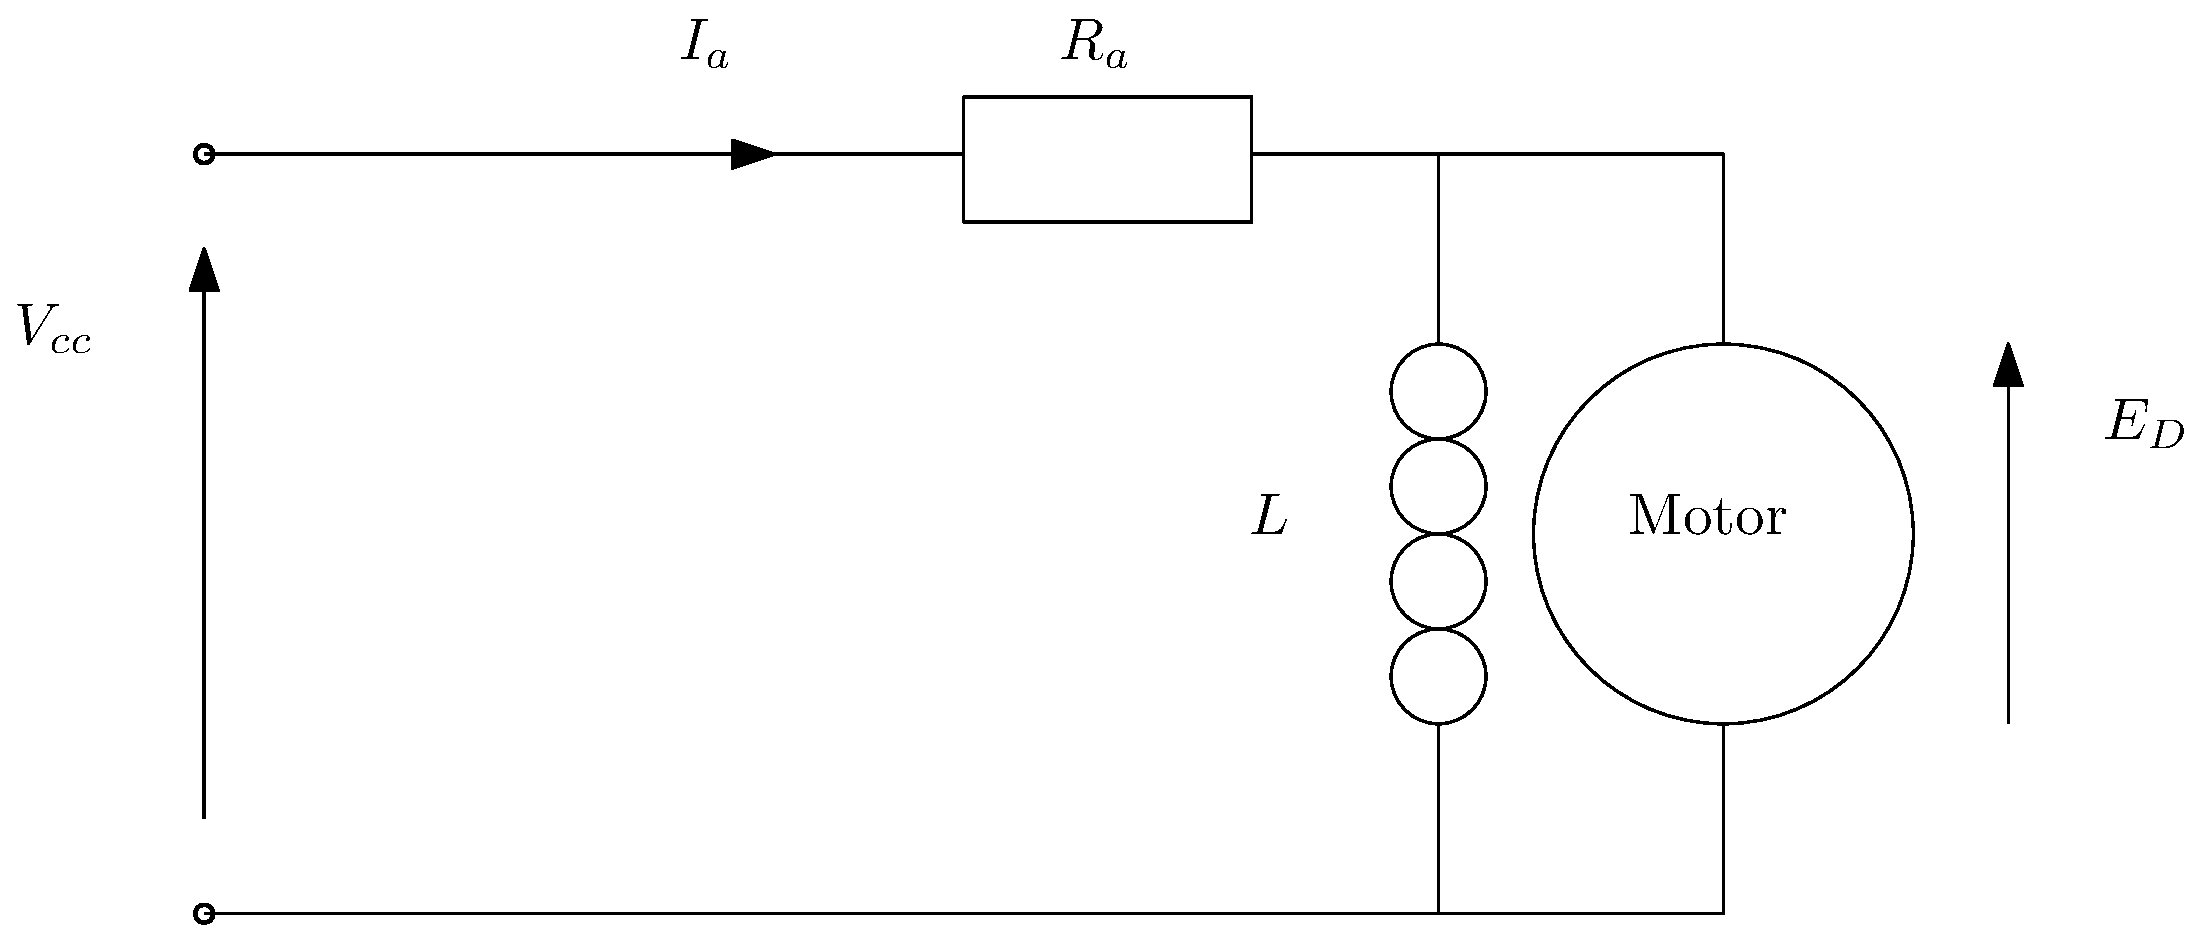
\includegraphics[width=0.9\linewidth]{dc_circuit.eps}
	\caption{Steady state equivalent circuit for a DC motor.}
	\label{fig:dc_circuit}
\end{figure}

This simple circuit leads to the relationship between current and internal resistance given by Equation \ref{eq:steady_state}.
\begin{equation}
V_{cc} = E_D + I_a R_a
\label{eq:steady_state}
\end{equation} 
It should be noted that the brushless DC motor is sometimes grouped with AC machines such as the induction motor due to its varying excitation \cite{Sarlioglu2016}. The coils are energised in order to keep the magnetic field at 90 degrees to the field generated by the permanent magnets mounted on the rotor. 

The field strength of the magnets, the number of poles and the number turns of the armature coils can be captured in the motor constant $k_T $ relating torque to armature current.

\begin{equation}
\tau = k_T I_a
\label{eq:torque_constant}
\end{equation} 

\begin{equation}
 E_D = \frac{rpm}{k_e}
\label{eq:emf_constant}
\end{equation} \\

 There are numerous loss sources in an electric motor such as winding resistance, flux leakage, eddy currents in the core and so on \cite{Sarlioglu2016}. By using real-world measured mechanical power output and electrical input, an equivalent winding resistance $R_a$ for the simple model can be found. The parameters are shown in Table \ref{tab:motor_params}. 
 
 \begin{table}
 	\caption{Motor parameters used in simulation.}
 	\label{tab:motor_params} 
 	\centering
 	\begin{tabular}{ |c|c| }
 		\hline
 		$k_v$ [rpm/v]& 6 \\ 
 		$k_T$ [Nm/A] & 1.53 \\ 
 		$P_{mech}$@375rpm [kW] & 3.6 \\ 
 		$P_{elec}$@375rpm [kW]& 6.37 \\
 		*$R_a$ [Ohms] & 1.0 \\
 		\hline
 	\end{tabular}
 \end{table}

\subsection{Air Resistance}
In addition to the resistive losses in the motor windings losses due to air resistance were also modelled. AGVs  typically operate at low speed <3m/s, hence the unaerodynamic shape of many models. However, the target speed of 10m/s is quite high around 30 miles per hour and drag could become significant. 

The drag coefficient $C_{drag}$=1 for a cuboid shape was used, taken from \cite{Toolbox2004}. The frontal area $A$ of 1m$^2$ is consistent with a box shape for maximum load carrying capacity. The density of air at room temperature is close to 1kg/m$^3$.

\begin{equation}
F_D = C_{drag} \rho v^2 A
\end{equation} 


\subsection{Arrival Distribution}
see Arrival Distribution for Intersection Simulation (Sources!).docx


\section{Methods For Zone-Based Intersection}
\subsection{Intersection Controller Objective}
The objective is to minimize $J_T$ the total travel time for all vehicles. It is convenient for exposition to optimize over the inverse of speed of each segment $\phi_k = 1/v_k$. Vehicle $i$ submits a plan containing $m_i$ segments before the conflict and $n_i$ segments in conflict. The control model is based on the average speed of each approaching AGV over each segment. This is to simplify the description of the intersection controller, and assist analysis. More sophisticated motion models could take the place of  Equation \ref{eq:omega_min} and  Equation \ref{eq:omega_max} to create a similar type of problem with a convex travel time objective and non-convex constraints.   
The parameters for one vehicle can be collected in the vector $\bm{\phi}_i$ as shown in Equation \ref{eq:phi_i}
\begin{equation}
\bm{\phi}_i =  [\phi_{1}, ..., \phi_{(m_i + n_i)}]^T \\
\label{eq:phi_i}
\end{equation}
The parameters for $p$ vehicles each traversing $(m_i + n_i)$ segments are assembled into a vector as in Equation \ref{eq:parameters}
\begin{equation}
\bm{\phi} = [\bm{\phi_{1}}^T, ..., \bm{\phi}_{p}^T]^T \\
\label{eq:parameters}
\end{equation}
Similarly, the length of each segment in plan $i$ can be arranged into a vector 
\begin{equation}
\bm{d}_i = [d_{1}, ..., d_{(m_i + n_i)}]^T \\
\label{eq:d_i}
\end{equation}
and collected  for $p$ vehicles into a vector as in Equation \ref{eq:d}.
\begin{equation}
\bm{d} = [\bm{d_{1}}^T, ..., \bm{d}_{p}^T]^T \\
\label{eq:d}
\end{equation}
This leads to the minimum travel time objective in Equation \ref{eq:qp_speeds}. 
\begin{equation}
\begin{array}{c}
\min \limits_{\bm{\phi}} \bm{J_T} = \bm{d}^T \bm{\phi} \\
\textrm{subject to}\\
 \bm{\phi}_{max} > \bm{\phi} > \bm{\phi}_{min} \\
 \bm{\phi}^T\bm{H}_{i,j}\bm{\phi} > \bm{0} \quad \forall i,j \in [1,p] \quad \textrm{with } j>i \\
\end{array}
\label{eq:qp_speeds}
\end{equation}

The condition $j>i$ in Equation \ref{eq:qp_speeds} indicates that the number of constraints varies with the number of vehicles $p$ as $\frac{p(p-1)}{2}$. This corresponds to one constraint between each pair of approaching AGVs.

\subsection{Intersection Controller Timing Constraints}
By definition, each intersection has a single conflict zone, the union of all segments which intersect there. This makes it possible to express the constraint that vehicles do not collide in terms of time. Vehicle $i$ arrives at the first conflicted segment $\omega_i^{min}$ and departs from the last at $\omega_i^{max}$. The following three subsections set out three alternative ways of expressing the collision avoidance constraints which have been evaluated. 
The arrival time is given by Equation \ref{eq:omega_min}. Considering average speeds, the departure time $\omega_i^{max}$ is also linear, this is given by Equation \ref{eq:omega_max}. 
\begin{equation}
\omega_i^{min}  = \sum_{k=1}^{m_i} \bm{d}_i [k] \bm{\phi}_i [k] = \bm{e}^T \bm{\phi}_i
\label{eq:omega_min}
\end{equation}
where %$\bm{e}[k] = \bm{d}_i[k] \forall k <m_i, otherwise 0$
\begin{equation}
\bm{e}[k] = \left\{
\begin{array}{cc}
\bm{d_i}[k] & \forall k <m_i \\
0 & \textrm{otherwise} \\
\end{array}
\right.
\end{equation}  and $m_i$ is the number of segments on the path of vehicle $i$ before arrival at the conflicted segment. 
\begin{equation}
\omega_i^{max}  = \omega_i^{min} + \sum_{i=1}^{n_i} \bm{d}_i [k] \bm{\phi}_i [k] = \bm{f}^T \bm{\phi}_i
\label{eq:omega_max}
\end{equation}
where 
\begin{equation}
\bm{f}[k] = \left\{
\begin{array}{cc}
\bm{d_i}[k] & \forall k <m_i+n_i \\
0 & \textrm{otherwise} 
\end{array}
\right.
\end{equation}
 and $n_i$ is the number of segments on the path of vehicle $i$ which are conflicted. Note that Equations \ref{eq:omega_min} and \ref{eq:omega_max} only depend on the $\bm{\phi}_i$ of vehicle $i$. 



\subsubsection{Linear FIFO Constraints}
\label{sec:fifo_constraints}
If the order in which the AGV cross the conflict zone is fixed to be First-In-First-Out, the timing constraint is linear. There is one constraint between each adjacent pair so $p-1$ constraints total for $p$ vehicles. These can be expressed in the form $\bm{A}_{ub}\phi \leq \bm{b}_{ub}$  as in Equation \ref{eq:fifo}. This is correct for two AGV arranged in distance order, each traversing one approach and one conflict segment. 

\begin{equation}
\left[ 
\begin{array}{ccccc}
-d_1 & 0 & d_3 & d_4 \\
\vdots 
\end{array} \right]
\left[
 \begin{array}{c}
  \phi_1 \\ \phi_2 \\ \phi_3 \\ \phi_4
 \end{array} \right]
\leq
\left[ 
\begin{array}{c}
0 \\ \vdots
\end{array} \right]
\label{eq:fifo}
\end{equation}

 The timing constriant between each pair of vehicles can be expressed with a modulus operator as in Equation\ref{eq:timing}.
\begin{equation}
|\alpha_i - \alpha_j| > \beta_i + \beta_j
\label{eq:timing}
\end{equation}

Here 
\begin{equation}
\alpha_i  = \omega_i^{max} + \omega_i^{min}
\label{eq:alpha}
\end{equation}
represents the midpoint of the time vehicle $i$ occupies the conflicted segment and
\begin{equation}
\beta_i  = \omega_i^{max} - \omega_i^{min}
\label{eq:beta}
\end{equation}
represents the range of the time either side of the midpoint, both scaled by a factor of two. 


In matrix form
\begin{equation}
\alpha_i  = \bm{f}^T \bm{\phi}_i + \bm{e}^T \bm{\phi}_i = \bm{1}_i^T\bm{A}{\phi}_i
\label{eq:alpha_m}
\end{equation}
with $\bm{A} = diag(\bm{f} + \bm{e})$
\begin{equation}
\beta_i  = \bm{f}^T \bm{\phi}_i - \bm{e}^T \bm{\phi}_i =  \bm{1}_i^T\bm{B}{\phi}_i
\label{eq:beta_m}
\end{equation}
with $\bm{B} = diag(\bm{f} - \bm{e})$

The resulting linear program (with parameters $\in\mathbb{R}$) has $p-1$ constraints as each AGV is only constrained by the preceeding one.

\subsubsection{Quadratic Constraints}
\label{sec:quad_constraints}
Another way to treat the modulus operator in Equation \ref{eq:timing}, without forcing any particular arrival order is to square both sides as to give the expression in Equation \ref{eq:expanded}. 
\begin{equation}
\alpha_i^2 - \alpha_j^2 - 2 \alpha_i\alpha_j - (\beta_i^2 + \beta_j^2 +2 \beta_i \beta_j) > 0
\label{eq:expanded}
\end{equation}
Collecting terms by subscript gives
\begin{equation}
(\alpha_i^2 - \beta_i^2) - (\alpha_j^2 + \beta_j^2) - 2(\alpha_i\alpha_j + \beta_i \beta_j) > 0
\label{eq:collected}
\end{equation}

The matrix $\bm{\Lambda}_ij$ captures the constraints between a pair of vehicles and always contains four sub-matrices as shown in in Equation \ref{eq:lambda}. It is compatible with $\bm{\phi}_{i,j} = [\bm{\phi}_i^T, \bm{\phi}_j^T]^T$, containing only the relevant speeds for vehicles $i$ and $j$. 
\begin{equation}
\bm{\Lambda}_{ij} =\left[
	\begin{array}{cc}
\bm{\Lambda}_{ij}^{ii} & \bm{\Lambda}_{ij}^{ij} \\
\bm{\Lambda}_{ij}^{ji} & \bm{\Lambda}_{ij}^{jj} \\
	\end{array}
	\right]
\label{eq:lambda}
\end{equation}
Expanding 
\begin{multline}
\left[\bm{\phi}_i^T, \bm{\phi}_j^T\right]
 \left[\begin{array}{cc}
\bm{\Lambda}_{ij}^{ii} & \bm{\Lambda}_{ij}^{ij} \\
\bm{\Lambda}_{ij}^{ji} & \bm{\Lambda}_{ij}^{jj} \\
	\end{array}\right]
\left[\begin{array}{c}
\bm{\phi}_i\\
 \bm{\phi}_j \end{array} \right] \\
= \bm{\phi}_{i}^T \bm{\Lambda}_{ij}^{ii} \bm{\phi}_{i} + \bm{\phi}_{j}^T \bm{\Lambda}_{ij}^{jj} \bm{\phi}_{j} + \bm{\phi}_{i}^T \bm{\Lambda}_{ij}^{ij} \bm{\phi}_{j} + \bm{\phi}_{j}^T \bm{\Lambda}_{ij}^{ji} \bm{\phi}_{i}
\end{multline}
 makes it possible to compare terms with the scalar expression in Equation \ref{eq:collected}. This leads to the following expressions for the submatrices in $\Lambda$ in terms of $\alpha_i = \bm{1}_T\bm{A}_i\bm{\phi}_i$ and $\beta_i = \bm{1}_T\bm{B}_i\bm{\phi}_i$ 
\begin{equation}
\bm{\Lambda}_{ij}^{ii} = (\bm{A}_i - \bm{B}_i)\bm{1}_i\bm{1}_i^T(\bm{A}_i - \bm{B}_i) 
\label{eq:ii}
\end{equation}
\begin{equation}
\bm{\Lambda}_{ij}^{jj} = -(\bm{A}_j + \bm{B}_j)\bm{1}_j\bm{1}_j^T(\bm{A}_J + \bm{B}_j) 
\label{eq:jj}
\end{equation}
\begin{equation}
\bm{\Lambda}_{ij}^{ij} + \bm{\Lambda}_{ij}^{ij T} = -2(\bm{A}_j + \bm{B}_j)\bm{1}_j\bm{1}_i^T(\bm{A}_i + \bm{B}_i) 
\label{eq:ij}
\end{equation}

For more than two vehicles this can be arranged into a block diagonal matrix $\bm{H}_{ij}$ which is compatible with the input parameters, but still only represents the constraints between a pair. 

Expressed in this way it is clear the constraints are quadratic and it is trivial to differentiate twice to find the Hessian is the stack of constraint matrices $[\bm{H}_{ij}, \hdots]$. The objective is certainly convex as it is linear but the constraints may not be. If the Hessian of the constraints is positive semi-definite then they are convex and interior point methods will either find the global optimum or prove that there is no feasible solution \cite{Boyd2004}. The Hessian depends on the parameters of the roadmap, the number of approaching vehicles and their distance from the conflict. 

\subsubsection{Mixed Integer Constraints}
\label{sec:milp_constraints}
A third way of treating the timing constraint in Equation \ref{eq:timing}, also without forcing any particular arrival order involves splitting each constraint into two based on the sign of $(\alpha_i-\alpha_j)$ as shown in equation \ref{eq:or_cons}. Again, this is expressed in terms of the midpoint $\alpha_i$, $\alpha_j$ and extent $\beta_i$,$\beta_j$ of the time when vehicle $i$ and vehicle $j$ occupy the segment on their own path which passes through the conflict point,
\begin{equation}
\begin{array}{cc}
\alpha_i - \alpha_j > \beta_i + \beta_j &\textrm{if  }\alpha_i >\alpha_j  \\
\alpha_i - \alpha_j < -(\beta_i + \beta_j) & \textrm{otherwise}\\
\textrm{where } \alpha_i, \alpha_j, \beta_i, \beta_j >0
\end{array}
\label{eq:or_cons}
\end{equation}
In order to apply these OR constraints, an additional integer parameter $b_k$ can be introduced for each pair of AGV, along with an arbitrary large number $M$ as shown in Equation \ref{eq:big_m_cons}. 
\begin{equation}
\begin{array}{cc}
\alpha_i - \alpha_j + b_{i,j}M > \beta_i + \beta_j \\
\alpha_i - \alpha_j - (1-b_{i,j})M < -(\beta_i + \beta_j) \\
\textrm{where } b_{i,j}\in[0,1] \\
M>>\alpha_i, \alpha_j, \beta_i, \beta_j
\end{array}
\label{eq:big_m_cons}
\end{equation}
Now the problem is combinatorial rather than convex and appropriate methods must be used. These may be based on exhaustive search such as Branch-and-Bound, or solving a sequence of convex relaxations of the original problem \cite{Murray2010}. Combinatorial problems quickly become intractable for large numbers of variables, but in this case the underlying problem of arrival order is combinatorial, so exhaustive methods are needed to find the global minimum. 

It is possible to further assume every AGV travels at maximum speed once it reaches the conflict, simplifying equation Equations \ref{eq:alpha} and \ref{eq:beta} with a constant $p_i = g_i \phi_{min}$. 
\begin{equation}
\alpha_i = 2\omega_i^{min} + p_i
\end{equation}
\begin{equation}
\beta_i = p_i
\end{equation}
 where $g_i$ is the length of the conflicted segments in the plan of vehicle $i$. In this case Equation \ref{eq:big_m_cons} can be restated 
\begin{equation}
\begin{array}{cc}
\omega_i^{min} - \omega_j^{min} + b_{i,j}M > p_j \\
\omega_i^{min} - \omega_j^{min}  - (1-b_{i,j})M < -p_i \\
\textrm{where } b_{i,j}\in[0,1] \\
\end{array}
\label{eq:minlp}
\end{equation}

\section{Methods For Conflict Point Intersection}
For a intersection between roads with multiple lanes, it makes sense to plot the centreline of each lane, and the arc of each turning motion between lanes. Any point where two of these arcs cross is called a conflict point. By controlling arrival time at a conflict point, collisions can be avoided, while vehicles that do not pass the same conflict point can both proceed \cite{Levin2017}.

\begin{figure}[ht]
	\centering
	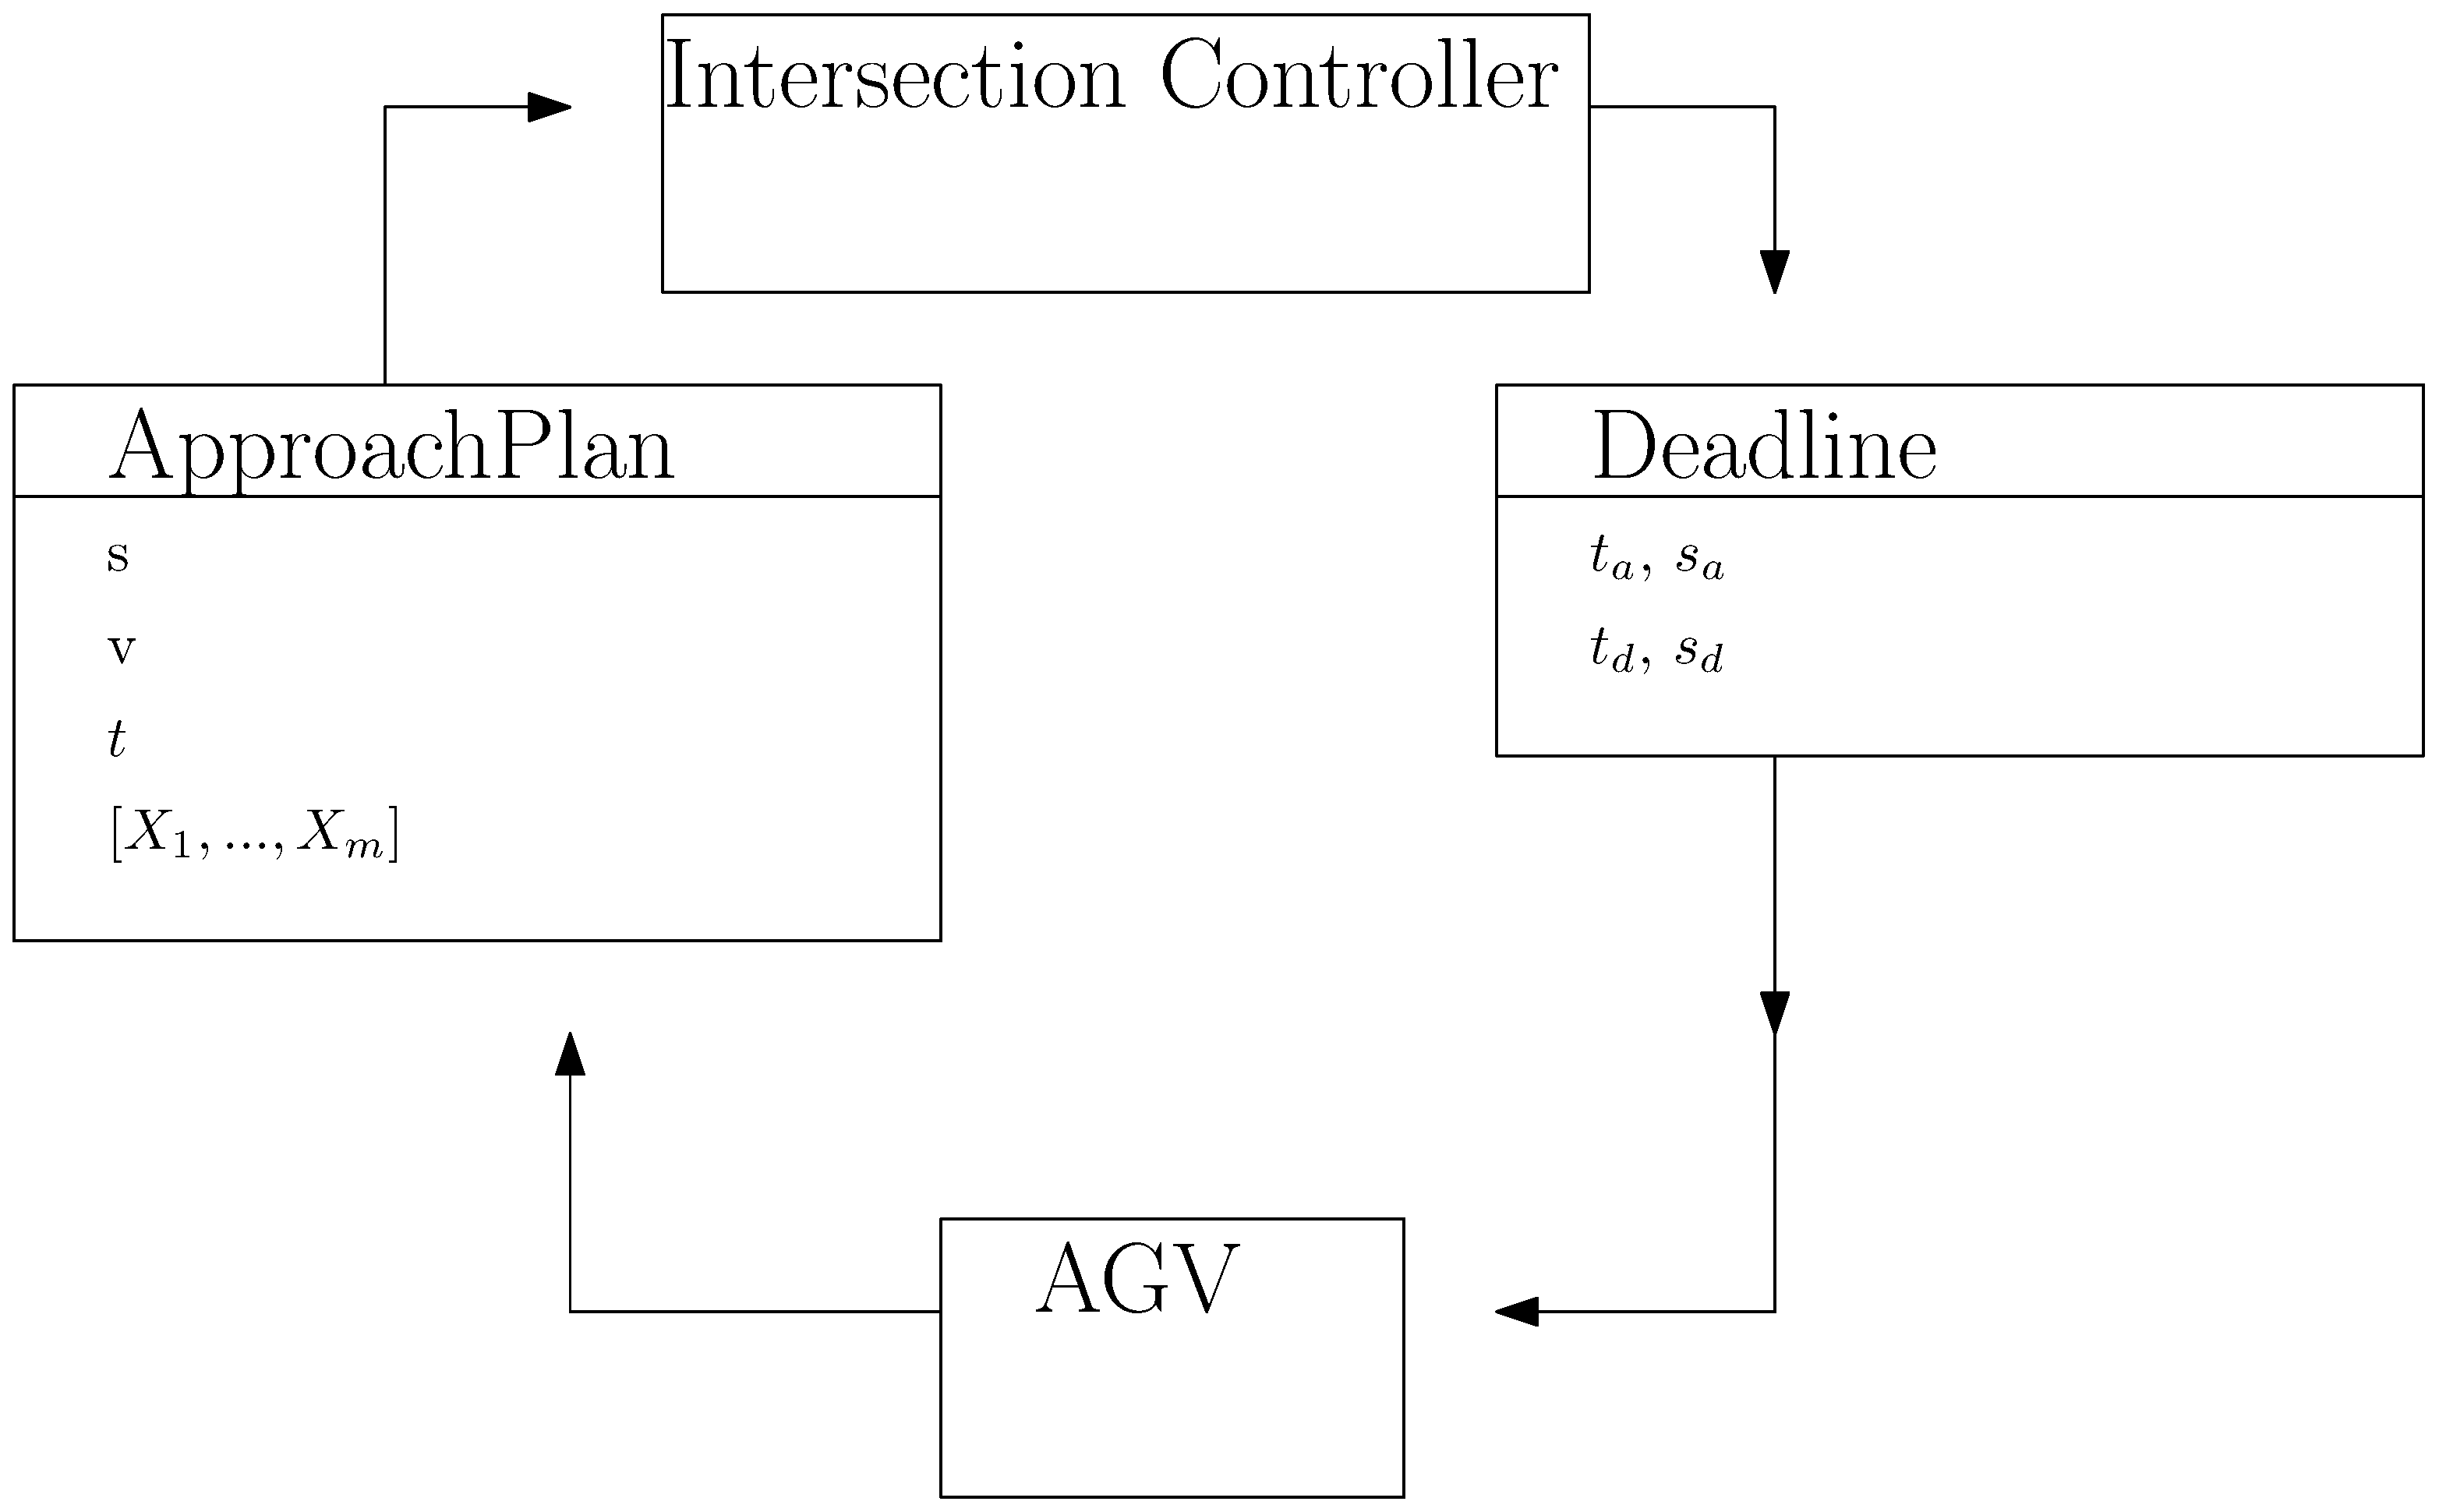
\includegraphics[width=0.9\linewidth]{plan_deadline_interface.eps}
	\caption{Key messages of the ``Plan/Deadline'' interface governing access to a conflict point intersection.}
	\label{fig:plan_deadline_interface}
\end{figure}

The design of an optimal intersection controller for a conflict point is very similar to that for an exclusion zone. A controller based on a common heuristic for controlling access to a shared resource, the binary semaphore, is included for comparison with the optimal methods.  Similar approaches are widespread in AGV control \cite{Duinkerken1999} and \cite{Lee2019}.
 
  
\subsection{Semaphore Approach}
 To implement the ``plan/deadline'' interface, a binary semaphore for each conflict point was needed. The semaphore controller does not compute the entry and exit times of the conflict as it has is no model of the vehicle dynamics. It simply raises the semaphore, sending a ``full speed ahead'' message to the closest AGV to the intersection and a position deadline to all others.
 
 For this reason the deadline message contains the position at which the agv must stop, without any timing. The AGV must stop at the given position until it receives a 'proceed' message form the intersection controller.
%=== Chapter Three ===
\chapter{Fitting Smooth Arcs to Polygon Regions - Comparative Results}

\section{Introduction}
To understand the advantages of using clothoid pieces to join two poses in a 2D obstacle field, it is informative to compare the output paths with an alternative curve type. One well known option is to use polynomial curves of  degree 3. 

\section{Methodology}
The paths are compared on two simulated environments. One is dimensioned for a small AGV with turning radius 0.5m, as might be used to deliver small items in a flexible manufacturing environment. The unexpected obstacle completely blocks the path to the right as in Figure \ref{fig:env1}. The second could represent a fork lift type AGV with a larger turning radius of 2m, which is collecting standard size (1m x1.2m) pallets from a storage area. See Figure \ref{fig:env1}. The pallets are placed by human drivers, and a reliable system fo detecting their position and orientation is assumed to be in place. The AGV must manoeuvrer to the pose of a target pallet, without colliding with the others. Lower curvature and sharpness allow the AGV to traverse the path faster without compromising load stability.

\section{Algorithm}
Both methods decompose the problem into topology followed by curve fitting. The topology problem is a posed as a directed graph with weighted edges. There is a node for every intersection of the boundary between two regions. Nodes within the same region are fully connected. The weight of each edge corresponds to the euclidean distance between the two nodes. The A* Algorithm is used to search for the set of edges which give the minimum sum of weights between any start and end pose.

The sequence of edges is then used to populate the matrix $\bm{H} ^{(R \times P)} \in [0,1]$. This is a binary matrix containing $R$ columns, one for each of the $R$ polygonal regions which comprise the accessible space. Each row corresponds to one of the $P$ path pieces and contains a single non-zero element indicating the region to which is assigned. A path piece may be present in more than one region as the regions may be overlapping, but it must always remain completely inside its assigned region.

\subsection{Polynomial Method}
The problem specification calls for a path which changes smoothly in x, y, heading and curvature. This should start at a specified $x_s, y_s, \psi_s$ with zero curvature and end at $x_g, y_g, \psi_g$ with zero curvature.

\begin{equation}
\begin{array}{c}
x(t) = a + bt + ct^2 + dt^3 \\
y(t) = e + ft + gt^2 + ht^3 \\
\end{array}
\label{eq:spline}
\end{equation}

There is a unique solution for a cubic spline of with fixed (x, y, heading) at the start and goal, passing through fixed $x, y$ positions numbering $n$. A cubic spline defined by Equation \ref{eq:spline} has eight free parameters per segment. To give a unique solution, eight constraints are must be found for each segment. Passing through the $n$ waypoints at the end of each segment gives two, one for the $x$ coordinate and one for $y$. Enforcing continuity of position between the end of each segment and the next leads to two more. Four more can be determined from continuity in the first and second derivative of position for a total of eight. 

However, only four constraints are needed at the start and end of the spline. Fixing the final position and heading, the acceleration must be left free. Stacking the parameters into a vector 
\begin{equation}
\bm{p}_i = [a_i, b_i, c_i, d_i, e_i, f_i, g_i]^T
\end{equation} 
and 
\begin{equation}
\bm{p} = [\bm{p}_1,\cdots,\bm{p}_i, \cdots, \bm{p}_{n-1}]^T
\end{equation} 
leads to the system of linear equations is given in Equation \ref{eq:assembled}. 

\begin{equation}
[\bm{A}|\bm{b}_{x}] = \left[\begin{array}{cccccc|c}
\bm{A}_{0} & & & & \cdots & 0 & \bm{b}_{x0}\\
\bm{0} & \bm{A}_{1} & & & \cdots & 0 & \bm{b}_{x1}\\
\vdots & 	& \ddots &	& 	& \vdots	& \vdots \\
0 & & \cdots & \bm{A}_{i} &  \cdots & 0 & \bm{b}_{xi}\\
\vdots & 	& 	&	& \ddots  &		& \vdots \\
0 & \cdots &  &  & &  \bm{A}_{n} 			& \bm{b}_{xn}\\
\end{array}\right] 
\label{eq:assembled}
\end{equation}

Where
\begin{equation}
[\bm{A}_{0}|\bm{b}_{x0}] = \left[ \begin{array}{cccc|c}
1 & 0 & 0 & 0 & x_0\\
0 & 1 & 0 & 0 & \cos{\phi_0}\\
\end{array} \right] 
\label{eq:submatrix_0}
\end{equation}

\begin{equation}
[\bm{A}_{i}|\bm{b}_{xi}] = \left[\begin{array}{cccccccc|c}
1 & 1 & 1 & 1 & 0 & 0 & 0 & 0 & x_{i}\\
1 & 1 & 1 & 1 & -1 & 0 & 0 & 0 & 0\\
1 & 1 & 2 & 3 & 0 & -1 & 0 & 0 & 0\\
0 & 0 & 2 & 6 & 0 & 0 & -2 & 0 & 0
\end{array}\right]
\label{eq:submatrix_i}
\end{equation}

\begin{equation}
[\bm{A}_{n}|\bm{b}_{xn}] = \left[\begin{array}{cccccccc|c}
0 & 0 & 0 & 0 & 1 & 1 & 1 & 1 &x_n\\
0 & 1 & 0 & 0 & 0 & 1 & 2 & 3 & \cos{\psi_n}\\
\end{array}\right] 
\label{eq:submatrix_n}
\end{equation}

The $\bm{p}_x$ parameters to fit a set of $n$ waypoints can be found by computing $\bm{p}_x = \bm{A}^{-1}\bm{b}_x$. The $\bm{p}_y$ parameters can be found almost identically, by computing $\bm{p}_y=\bm{A}^{-1}\bm{b}_y$. Constraint vector $\bm{b}_y$ is instead constructed using the $y$ coordinates of the waypoints in $b_i$ and the $\sin$ of the start and end heading in $\bm{b}_{y0}$ and $\bm{b}_{yn}$.

\section{Optimisation}
The point to point solution through the region intersection points is quite a good solution. Continuous in $\dot{X}$ and $\ddot{X}$, it reaches the goal position and heading. It is excessively constrained by the requirement to meet the intermediate waypoints.
Using the optimisation in Equation \ref{eq:full_opt}  
\begin{equation}
\begin{array}{c}
\min \sum_{j=1}^N ||\frac{dP_j^3(t)}{dt^3}||^2 \\
\textrm{subject to} \\
P_j(1) = P_{j+1}(0) \\
\dot{P_j}(1) = \dot{P_j}(0) \\
\ddot{P_j}(1) = \ddot{P_j}(0) \\
P_1(0) = X_S \\ 
P_N(1) = X_G \\
\dot{P_1}(0) = \dot{X_S} \\
\dot{P_N}(1) = \dot{X_G} \\ 
\textrm{also subject to} \\
\bm{H}_{j,r} \Rightarrow X_r^{min} \leq P_j(t) \leq X_r^{max} 
\end{array}
\label{eq:full_opt}
\end{equation}

The implementation of the region constraint in Equation \ref{eq:full_opt} must ensure the entire arc remains inside the assigned region according to $\bm{H}$. For piecewise linear arcs this can be done by checking the containment of the start $P_0(0)$ and end $P_N(1)$. Got cubic splines it is more challenging. Deits and Tedrake \ref{Deits2015} describe an approach based on Sum of Squares, where a small Semidefinite Program is solved in the parameters of $P_j$, to avoid sampling at different $t$ values, which can lead to the path cutting corners and even passing through thin obstacles.

First we notice that the constraints on one segment from its axis aligned containing region described by $x_min, x_max, y_min, y_max$ can be written as vector inequality
\begin{equation}
 q(t) = \left[\begin{array}{c}
 x_{max} - a - bt - ct^2 - dt^3 \\ 
 a + bt+ ct^2 + dt^3 - x_{min} \\
 y_{max} - e - ft - gt^2 - ht^3 \\ 
 e + ft+ gt^2 + ht^3 - y_{min} \\
 \end{array}\right] \geq \bm{0} \forall t \in [0,1]
 \label{eq:qt}
 \end{equation}
. The condition in Equation \ref{eq:qt} can only hold if and only if it can be rewritten in the form
\begin{equation}
t\sigma_1(t) + (1-t)\sigma_2(t)
\end{equation}
. This leads to 
\begin{equation}
\sigma_1(t) = \left[\begin{array}{c}
	x_{max} - a- b- ct- dt^2 \\
	a + b+ ct+ dt^2 - x_{min} \\
	y_{max} - e - f - gt - ht^2 \\
	e + f+ gt+ ht^2 +-y_{min} \\
	\end{array}\right]
\end{equation}
and 
\begin{equation}
\sigma_2 = \left[\begin{array}{c}
x_{max} -a \\
a - x_{min} \\
y_{max} - e \\
e - y_{min} \\
\end{array}\right]
\end{equation}. 
The standard Sum of Squares approach calls for collecting the parameters of $\sigma(t)$ by the order of $t$. Matching coefficients against
\begin{equation}
\sigma_i = \beta_1 + \beta_2 t + \beta_3 t^2
\end{equation}, gives
\begin{equation}
\beta_1 = \left[\begin{array}{c}
x_{max} - a - b \\
a + b - x_{min} \\
y_{max} - e - f \\
e + f + y_{min} \\
x_{max} - a \\
a - x_{min} \\
y_{max} - e \\
e + y_{min} \\
\end{array}\right]
\end{equation}
and
\begin{equation}
\beta_2 = \left[\begin{array}{c}
-c \\
+c  \\
-c \\
+c \\
0\\
0 \\
0 \\
0 \\
\end{array}\right]
\end{equation}
and
\begin{equation}
\beta_3 = \left[\begin{array}{c}
-d \\
+d  \\
-d \\
+d \\
0\\
0 \\
0 \\
0 \\
\end{array}\right]
\end{equation}
. Where the parameters for $\sigma_2$ have been stacked after those from $\sigma_1$. 

In order for $\sigma_i$ to be a sum of squares, there are the following conditions on $\beta_1$, $\beta_2$, $\beta_3$:
\begin{equation}
\begin{array}{c}
4\beta_1\beta_3 - \beta_2^2 \geq 0
\beta_1, \beta_3 \geq 0
\end{array}
\end{equation}

 In the simple case where the regions are axis aligned, this immediately creates a problem as the first two equations have $\beta_3 = d$ and $\beta_3 = -d$. The only value of $d$ which will satisfy the sum of squares condition is zero. However the initial guess which joins the corner points, satisfies the region occupancy constraints with a non-zero $d$. 
 
 For this reason the constraints are enforced using 50 samples for each path piece. This leads to a small degree of corner cutting which must be included in the safety factor used on the vehicle body width used to inflate the obstacle. It also results in a large number of constraints as there are four for each sample. For this to be possible we must use a fixed spatial sampling length rather than a fixed number of samples per piece as path pieces can vary in length substantially which makes the degree of corner cutting variable.
 



\subsection{Clothoid Method}
Initialization with parameters which meet the continuity and obstacle constraints with clothoid pairs proved to be a challenging task. This is expected to improve the convergence time. To generate a set of parameters to meet continuity constraints for initialization of the region method is very similar to the interpolation problem addressed by Bertolazzi et al (2018) \cite{Bertolazzi2018}. The main difference is that the intermediate waypoint headings are free variables in the initialization, unlike in interpolation.

If the waypoint headings are fixed, and curvature at them to zero, the clothoid interpolation problem can be solved for each segment independently, as described by \cite{Gim2017a}. Different point to point methods could be used such as the bisection method \cite{Gim2017b}, geometry \cite{Vazquez-Mendez2016} and minimax sharpness \cite{Henrie2007}. Lacking a natural heading, a heuristic based on the maximum squared sum of $a^2 + b^2$ and requiring $a>0$ and $b<0$ where $a$ is the distance to the intersection point from $P_1$ and $b$ is the distance from $P_2$. The different sign is important for the direction of travel, to put the intersection in front of the first pose and behind the second.

The multiple shooting clothoid method uses additional parameters for the start pose of every segment. If this was initialized to zero, interior-point method reached convergence in about 70 seconds in environment 2. None of the more involved methods improved on this so we used the simple approach for further testing.  

\section{Convergence dependence on $b$}
\begin{figure}
	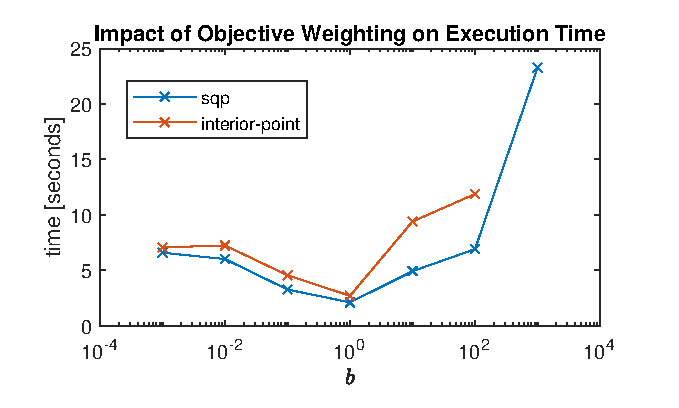
\includegraphics[width=0.5\linewidth]{w_convergence_time_SMALL}
	\label{fig:w_convergence}
	\caption{Convergence time variation with weighting on item fetch environment}
\end{figure}

In environment 1 both large and small values of $w$ led to poor convergence. One possible explanation is numerical conditioning being damaged by the weighting. A large $w$ results in a solution with small $\alpha$, while the length remains on the same order. Some matrix operations may return inaccurate results with different magnitude parameters.
\begin{table}
\begin{center}
	\begin{tabular}{ |c|c|c|c|c| }
		\hline
		 $b$ & $1\times10^{-3}$&  1 & 100 & 1000* \\ 
		 \hline
		 fevals &7929 & 10873 & 11986& 200,000* \\  
		 execution time (s)& 55 & 72 & 80 & 1345* \\
		 path length (m) & 7.071 & 11.694 & 36.038 & 5.695*\\
		 \hline  
	\end{tabular} \\
		 *Convergence Failure
\end{center}
\label{tab:b_dependence}
\caption{Convergence for different $b$ values for the multiple shooting approach, in pallet environment} 
\end{table}
To test the hypothesis that only method using dense matrices such as sqp would be affected, the effect on the interior point method (which does not depend on dense matrix operations) is reported in Table \ref{tab:b_dependence}. This shows that changing the weighting damages convergence significantly to the extent that no valid result is found even after 200000 function evaluations. There were no warnings printed by fmincon during this run. The value of feasibility was positive of the order 1e-6 and decreasing very slowly, while the objective function was large of the order 1e6 and also decreasing very slowly (relative to its magnitude).

Contrary to expectation, reducing $b$ to emphasize the path length reduced the number of iterations to convergence. Table  \ref{tab:b_dependence} shows an inverse relationship between $b$ and the number of iterations. Sufficiently large $b$ makes the problem more difficult to solve as the path segments deflect further, making a linear approximation worse. This effect is indirect because the constraints use the precise nonlinear dynamics and the interior-point method does not solve a series of linear approximations to the constraints like sqp. Interior point should always converge if given an initial guess in the feasible reason, unless the problem is non-convex. The initial graph step intended to remove non-convex elements of the problem may lead to suboptimal paths as the segments deviate from straight lines. But this does not explain the increasing number of iterations. 

Curvature is more weakly linked to the parameters than the total length. The curvature objective is the squared sum of $2r$ parameters while the length objective is the squared sum of $4r$ parameters. Both of them leave numerous parameters to be coupled through the constraints as in total there are $9r$ parameters for the multiple shooting formulation. 

\section{Generating a Convex Region Representation from LIDAR Data}
A widely used representation for a 2D obstacle field is an occupancy grid \cite{Thrun1996}. Also see Probabilistic Robotics textbook \cite{thrun2005probabilistic} for details on creating a map from sensor data. Each cell represents an area of the floor, with a number $p\in[0,1]$ indicating the probability it contains an obstacle. Thresholding can be used to create a binary map of occupied and unoccupied cells. In order to connect adjacent unoccupied cells to form regions numerous approaches from image processing are available. A method suitable for simple environments is vertical cell decomposition \cite{LaValle2006c}. This begins with piecewise linear polygons, which can be created by connecting the cell corners of a binary occupancy grid.


\section{Test Environment}
The test environment was created for an automated fork lift AGV research platform which is taken to be representative \cite{Baird2018}. The obstacles are based on $(1.0 \times 1.2)$m pallets which are commonly used in the UK and Netherlands \cite{Raballand2005}. The datasheet for the manually operated vehicle on which the AGV is based, a Hyster E30-40HSD gives the dimensions in Table \ref{tab:dimensions}. The dimensions are drawn on a plan of the vehicle in Figure \ref{fig:fork_dims_circ}.

\begin{figure}
	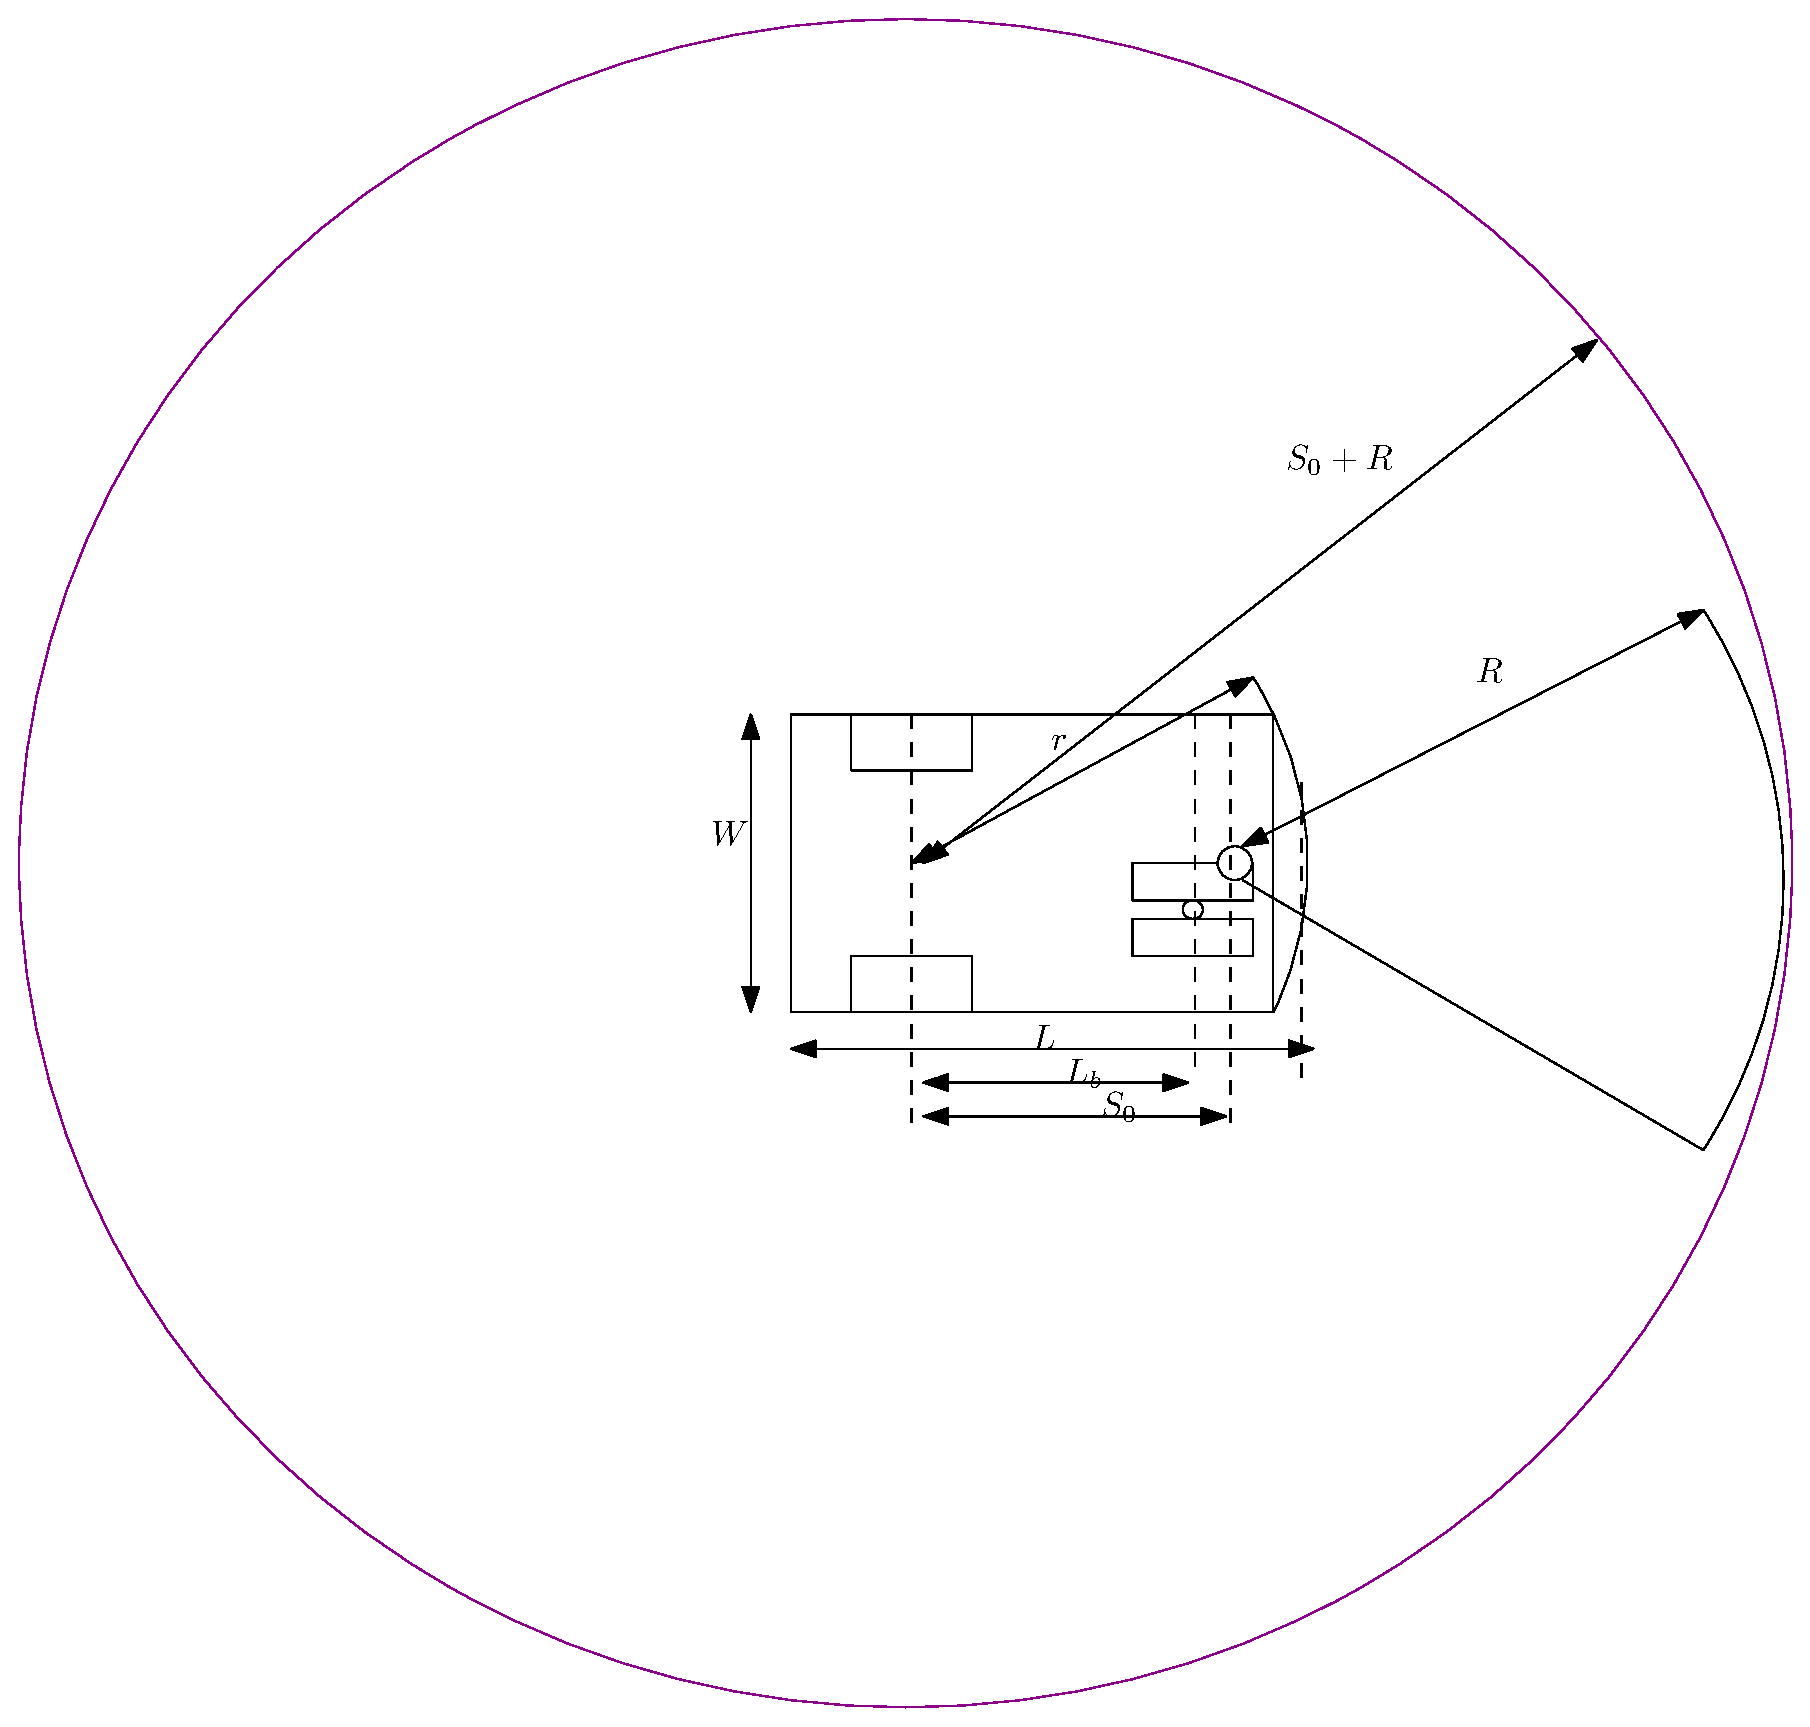
\includegraphics[width=0.5\linewidth]{fork_dims_circ}
	\label{fig:fork_dims_circ}
	\caption{Dimensions used to expand the obstacles}
\end{figure}
\begin{table}
	\begin{center}
		\begin{tabular}{ |c|c| }
			\hline
			Parameter & Dimension (mm) \\
			\hline
			$W$ & 1067 \\
			$L$ & 1583 \\
			$r$ & 1289 \\
			$L_s$ & 1001 \\
			$S_0$* & 1200 \\
			$R$* & 1300 \\
			\hline  
		\end{tabular} 
	\end{center}
	\label{tab:dimensions}
	\caption{Dimensions from datasheet. *Stopping distance $R$ based on top speed 3.22m/s and hypothetical braking deceleration of 4m/s$^2$} 
\end{table}
The datasheet gives the maximum speed as 7.2 miles per hour (3.22m/s). Traction is provided by dual 4.8kw motors. The unloaded weight of the vehicle is 3059kg and the battery 1043kg for a total of 4201kg.  

For correct operation it is important to consider the exclusion zone of the safety rated range sensor fitted to the front of the vehicle. If an obstacle breaches the exclusion zone the AGV must perform an emergence stop, or in some cases slow down significantly. To avoid slowing down the path planning must account for not only the shape of the vehicle but also the shape of this zone. Often this is a cuboid slightly wider than the vehicle, sufficiently long that the AGV can come to a complete stop from full speed before the front makes contact with a static obstacle. More details are available in the NIST Safety Standards \cite{Bostelmann2013}. To avoid 

In the two simulated environments the obstacle field is represented in 2D. The bounding circle dimension is strongly influenced by the stopping distance $R$. 
Starting from the constant acceleration equation
$v^2 = u^2  + 2as$ and setting $v=0$ gives the stopping distance $s = \frac{u^2}{-2a}$. 
\begin{figure}
	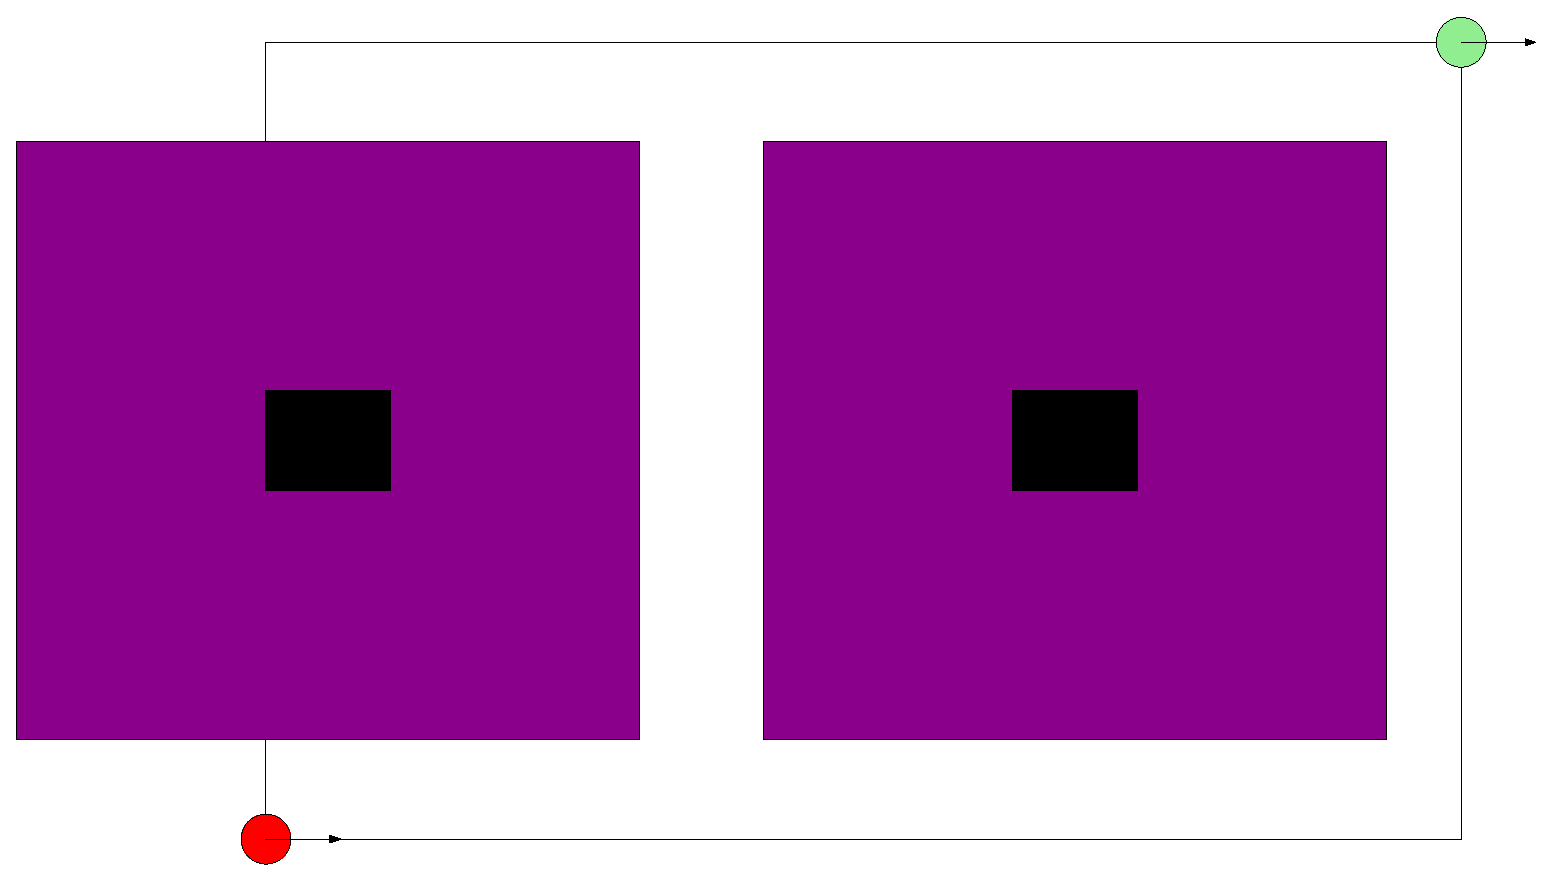
\includegraphics[width=0.5\linewidth]{pallet_env_expand_2point5}
	\label{fig:pallet_env}
	\caption{Pallet environment. Obstacles are black with expansion by the vehicle disk shown in purple.}
\end{figure}

Expanding the environment with a disc the size of the largest dimension of the vehicle is a gross approximation, which will lead to over cautious paths. It would be better to represent the obstacles in (2 + 1) dimensions, and plan in ($x, y, \psi$). Obstacles can then be expanded based on the current heading of the path as described in \cite{Deits2015b} who use a sum of squares approach to find (2+1)D convex polygons. 

%=== Chapter Four ===
\chapter{Intersection Control for Automated Vehicles }
\section{Introduction}
The capacity and safety of an intersection can be considered in terms of the number and type of conflict points which it contains. When every entrance to the intersection is connected to every exit by a smooth arc, a conflict point exists wherever two arcs intersect. They can be classified as head-on, following, crossing, diverging or merging. In many studies these points are assumed to be fixed, and only speed of the vehicles which controls the rate of progress along the arcs is varied to minimise delay. 

With the development of path planning around obstacles on-the-fly, it becomes possible to consider what arrangement of conflict points is best given the traffic at a particular instant in the near future. 

\section{Literature Review} 
Studies on the theoretical capacity of signalized intersections and roundabouts with an equivalent footprint indicate that in most cases, if there are few approach lanes small roundabouts will tend to have higher capacity. If there are many approach lanes signals tend to be more effective, unless the traffic on different approaches is extremely unequal \cite{Jian-an2001}. 

A systematic procedure computing the conflict points in an intersection is given in \cite{Lu2013}. Roundabouts tend to have a large number of merging and diverging conflicts, but fewer or none of the crossing and head-on conflicts which lead to the most serious collisions due to high relative speeds.

Intersection control often addresses crossing conflicts by separating vehicles in time, while they all take the shortest path straight through the intersection in the same way as if it was signal controlled. There are a wide range of optimal and heuristic approaches to solve for the speed profile, both decentralized and centralized, a good review is given in \cite{Rios-Torres2017}. Many studies have looked at how to incorporate a proportion of human controlled vehicles which are not able to communicate their intention. One way of doing this is using traffic signals which only apply to human drivers \cite{Zhao2019}. The downside is that the nature of the intersection must remain similar to a traffic-light controlled one if non-communicating participants are going to be controlled by lights.

Recently a number of studies have extended intersection coordination of Connected and Autonomous Vehicles (CAVs) to the resolve the type of merging of diverging conflicts which occur and roundabouts. These are reviewed in \cite{Rios-Torres2017}. A centralized solution with an intersection manager minimizing delay and energy consumption is described in \cite{Zhao2018}. This shows that a high proportion of vehicles need to be communicating for significant benefits to be realized. 

A decentralized approach based on intent communication by way of virtual vehicles, can also be applied to roundabouts. In \cite{Debada2016}, reactive heuristics are shown to lead to poor performance compared to a model predictive control approach. The virtual vehicle concept allows common lane based heuristics such as car following to be extended to resolve conflicts in  \cite{Debada2018}. Another work investigating virtual lanes is \cite{Xu2018}. Here a conflict graph is used to assign approaching vehicles to appropriate virtual lanes and a distributed controller is presented to stabilize the platoon.

Another approach presented in \cite{Liu2018} is a decentralized solution to the global problem of minimizing the delay. Proofs of completeness and optimality of the aggregate problem are given, making this technique very impressive. It is not shown to be applicable to roundabouts in any of the numerical examples, although the incorporation of optimal trajectory planning by the low level controller to execute merging makes it a good example of the combination of path planning and intersection management. Collision constraints are based on a conflict zone rather than conflict points as in \cite{Levin2017}. The location of the conflict points is fixed by the fixed paths between the entry and exit lanes of the junction. The space inefficiency of the zone representation for multiple lanes is addressed by using multiple zones, one for each pair of lanes. The use of simultaneous path optimization might be expected to increase computational complexity and thereby reduce the number of vehicles with can be routed, however an attached video showing many vehicles interacting for about 10 minutes seems to refute this. It seem the ordering problem is resolved in a decentralized way based on game theory and the game `Chicken.' Using game theory to resolve the ordering problem may give this approach an edge over the mixed integer optimization used in \cite{Levin2017}, in terms of how many vehicles they can control before running into execution time limits. It is a little surprising that the game would always produce the optimal ordering given the motion model used by each AGV. The consensus mechanism will be important here. Questions remain about the possibility of AGVs disagreeing about the order they calculate from the communicated position and speed data. 

A similar method which solves the ordering ordering problem sequentially, followed by individual optimization of the approach speed along fixed paths is described in \cite{DeCampos2017}. This method claims only local (per-vehicle) optimality for the speed choice sub problem, and makes it clear the crossing order at convergence will be suboptimal, and depends strongly on the decision order. The sub problem is posed as a Linear Quadratic Regulator, commonly seen in optimal control problems. In general terms, those early in the decision order will deviate from the plans less. This is more of a problem when vehicles are not uniform, as to reduce energy consumption a late arriving lorry should deviate as little as possible. A heuristic is given for the decision order based on the time to conflict arrival.

The use of optimal control in \cite{DeCampos2017} is shared with many earlier works regarding coordination of Unmanned Arial Vehicles, many of which relax the assumption of static paths. In this way \cite{Schouwenaars2004} addressed the full multi-vehicle motion planning problem for small numbers of aircraft with simple dynamics. The craft were assumed to be differentially flat: that is, able to actuate in any of the workspace degrees of freedom independently, like a quadrotor. They were represented using bounding rectangles, leading to a slightly conservative mixed integer problem. The integer variables are used to choose which constraints are active. This might seem excessive when representing static obstacles, however when the constraints arise from other moving vehicles, the integer variables are a natural way to represent the passing-order problem. The scaling to larger numbers of vehicles is a particular challenge, due to the combinatorial explosion of possibilities.

An alternative approach to the coordination of differentially flat aircraft which uses a sequential solution of per-vehicle receding horizon sub problems to approximate the global solution is given in \cite{Keviczky2008}. An earlier theoretical treatment based on iterative bargaining with soft collision constraints is given by \cite{Inalhan2002}. The parameters are real numbers, and the constraints linear while the cost is quadratic. It may converge to an infeasible solution given a particular minimum safety distance even from a valid set of starting positions and speeds, and the suggested solution is to reduce the threshold until it becomes feasible.  

More recently, solutions based on Distributed Model Predictive (DMPC) control have been developed. In \cite{Dai2017}, per-vehicle optimizations runs simultaneously to reduce execution time. This ensures recursive feasibility and closed loop stability. Another DMPC approach is given by \cite{Luis2018}. This scales up to 25 vehicles in real time. the quadrotors concerned are all identical and differentially flat. For an under-actuated system like an AGV, some of the simplifications may no longer be possible. 

%The distributed consensus on the arrival order underpins the distributed solution for trajectory planning. The body of work considering flexible paths for aircraft relies on similar techniques to the latest works targeted at Connected Automated Road Vehicles where the paths are fixed. Specifically \cite{Liu2018} uses sequential per-vehicle optimisation to find the highest safe speeds subject to static obstacle constraints, and the trajectories of vehicles earlier in the sequence. The crossing order is determined by the arrival time at the 'point of no return' according to the motion model of each vehicle. The high frequency closed loop controller on one vehicle continues to operate while the others are formulating their own trajectory plan. Similarly the work on adaptive paths in \cite{Luis2018} uses simultaneous per-vehicle optimisation to find the trajectory as a sequence of control actions and associated positions at regular time intervals which the vehicle is predicted to occupy up to a receding time horizon. Both offer a suboptimal global (all-vehicles) solution, which is guaranteed to be safe. Could the simultaneous approach improve performance of DMPC? Is it just a different name for the same algorithm? An existing constrained optimisation based path planner could be used to generate trajectories by assuming a simple speed profile. Mutual constraints between two trajectories can then be applied, with one constraint for each time sample, leading to a solution to the central(all-vehicle) multi-vehicle trajectory planning problem. The local(per-vehicle) optimization is identical to the global(all-vehicle) one, only the passing order choice need to reach consensus. Either of the two aforementioned decentralized ordering algorithms should be applicable. Which is most promising, resulting in a consensus with the least deviation from central(all-vehicle) optimality? Does the answer change depending on the nature of the path optimisation, should it be based on a clothoid spline or radial polynomials?

 

%==================


\section{Simulation}

Platooning with speed choice by a centralized controller was implemented with a vehicle to intersection messaging scheme. The full site is divided into zones, each one containing a single intersection. Each AGV in the fleet has a copy of the roadmap which is  static. The fleet controller interfaces with the warehouse management system to get the next material transfer job, consisting of a pick location and a drop location. All jobs are assumed to be of unit size and each AGV has a capacity of one unit. With these assumptions, a straightforward policy is to assign the next job to the AGV nearest to the pick location - first-come-first-served scheduling. When an AGV receives a new job, it finds the shortest path through the roadmap using the Floyd-Warshall algorithm \cite{Djojo2013}. Next it must send its planned path to the intersection controller for the zone it currently occupies. The intersection controller stores the plan and current position of every AGV approaching the conflict point of the intersection. Every time it receives a new plan it must recalculate the approach speed for every approaching AGV to minimize total travel time without collision. This will happen every time an AGV enters the zone from somewhere else, or an AGV within the zone is assigned a new job.

%\begin{figure}[ht]
%\centering
%\includegraphics[width=\linewidth]{intersection_layout_trim}
%\caption{Intersection layout shown in SUMO NETEDIT tool \cite{dlr2016}}
%\label{fig:layout}
%\end{figure}
\begin{figure}[ht]
	\centering
	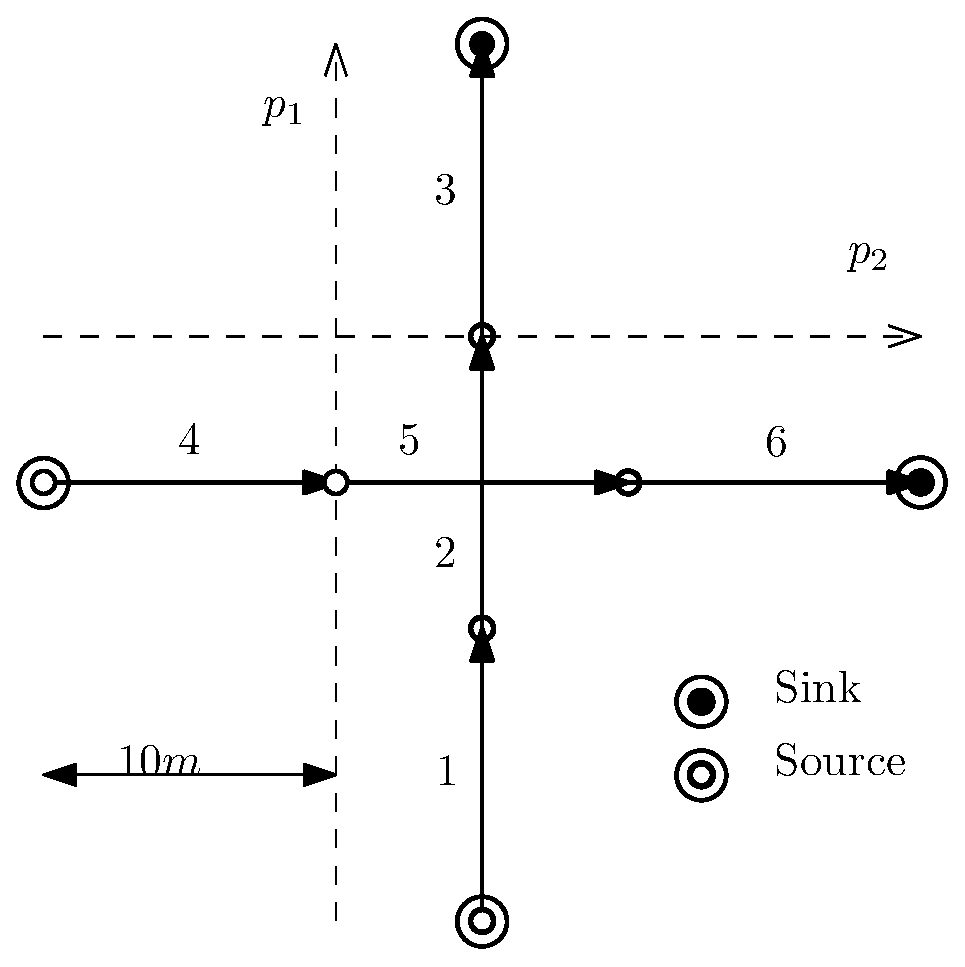
\includegraphics[width=0.9\linewidth]{intersection_topo}
	\caption{Intersection layout with two conflicting routes.}
	\label{fig:layout}
\end{figure}

The intersection controller was implemented based on \cite{Digani2019}. The surrounding lanes are first discretized into segments. The intersection shown in Figure \ref{fig:layout} is divided into six segments, each of length 10 meters. The critical segments are the two that cross in the center. There are two routes defined, one starting on the left and traveling to the right and the other starting at the bottom and traveling up. One AGV takes route 1 and the other takes route 2. If they both travel at maximum speed they will collide in the center.

The dynamic model for each AGV assumes they are able to exactly follow the path, and attempt to reach the target speed for each segment subject to a limited rate of acceleration of $a m/s^2$. 

\begin{figure}[ht]
	\centering
	\includegraphics[width=0.9\linewidth]{SystemSetup3.pdf}
	\caption{Messages exchanged by participants approaching intersection.}
	\label{fig:system_setup}
\end{figure}

The ApproachPlan message sent by the AGV contains a sequence of segments which it intends to traverse, along with its current distance along the first one.  The flow of messages is shown in Figure \ref{fig:system_setup}. The SpeedList sent by the intersection controller contains the optimal speed for every segment in the plan. The speeds can be found with the nonlinear program in Equation \ref{eq:qp_speeds}. 

\subsection{Motor Dynamic and Electrical Model}
The simulated AGV are based on a small payload 100kg total mass, with a maximum speed of 10m/s and peak acceleration of 5m/s$^2$, allowing them to stop safely within 10 metres. The intersection controllers use a constant acceleration model to calculate the time and space deadlines they pass to the AGV. To make the simulation test worthwhile a simulation model with slightly more complexity was used to evaluate the performance.


The brushless DC electric motor used in \cite{Racewicz2018} has suitable properties to propel a 100kg battery powered vehicle. A DC motor can be modelled by the steady state equivalent circuit shown in Figure \ref{fig:dc_circuit} which is well known, for example see \cite{Hughes2008}. 

\begin{figure}[ht]
	\centering
	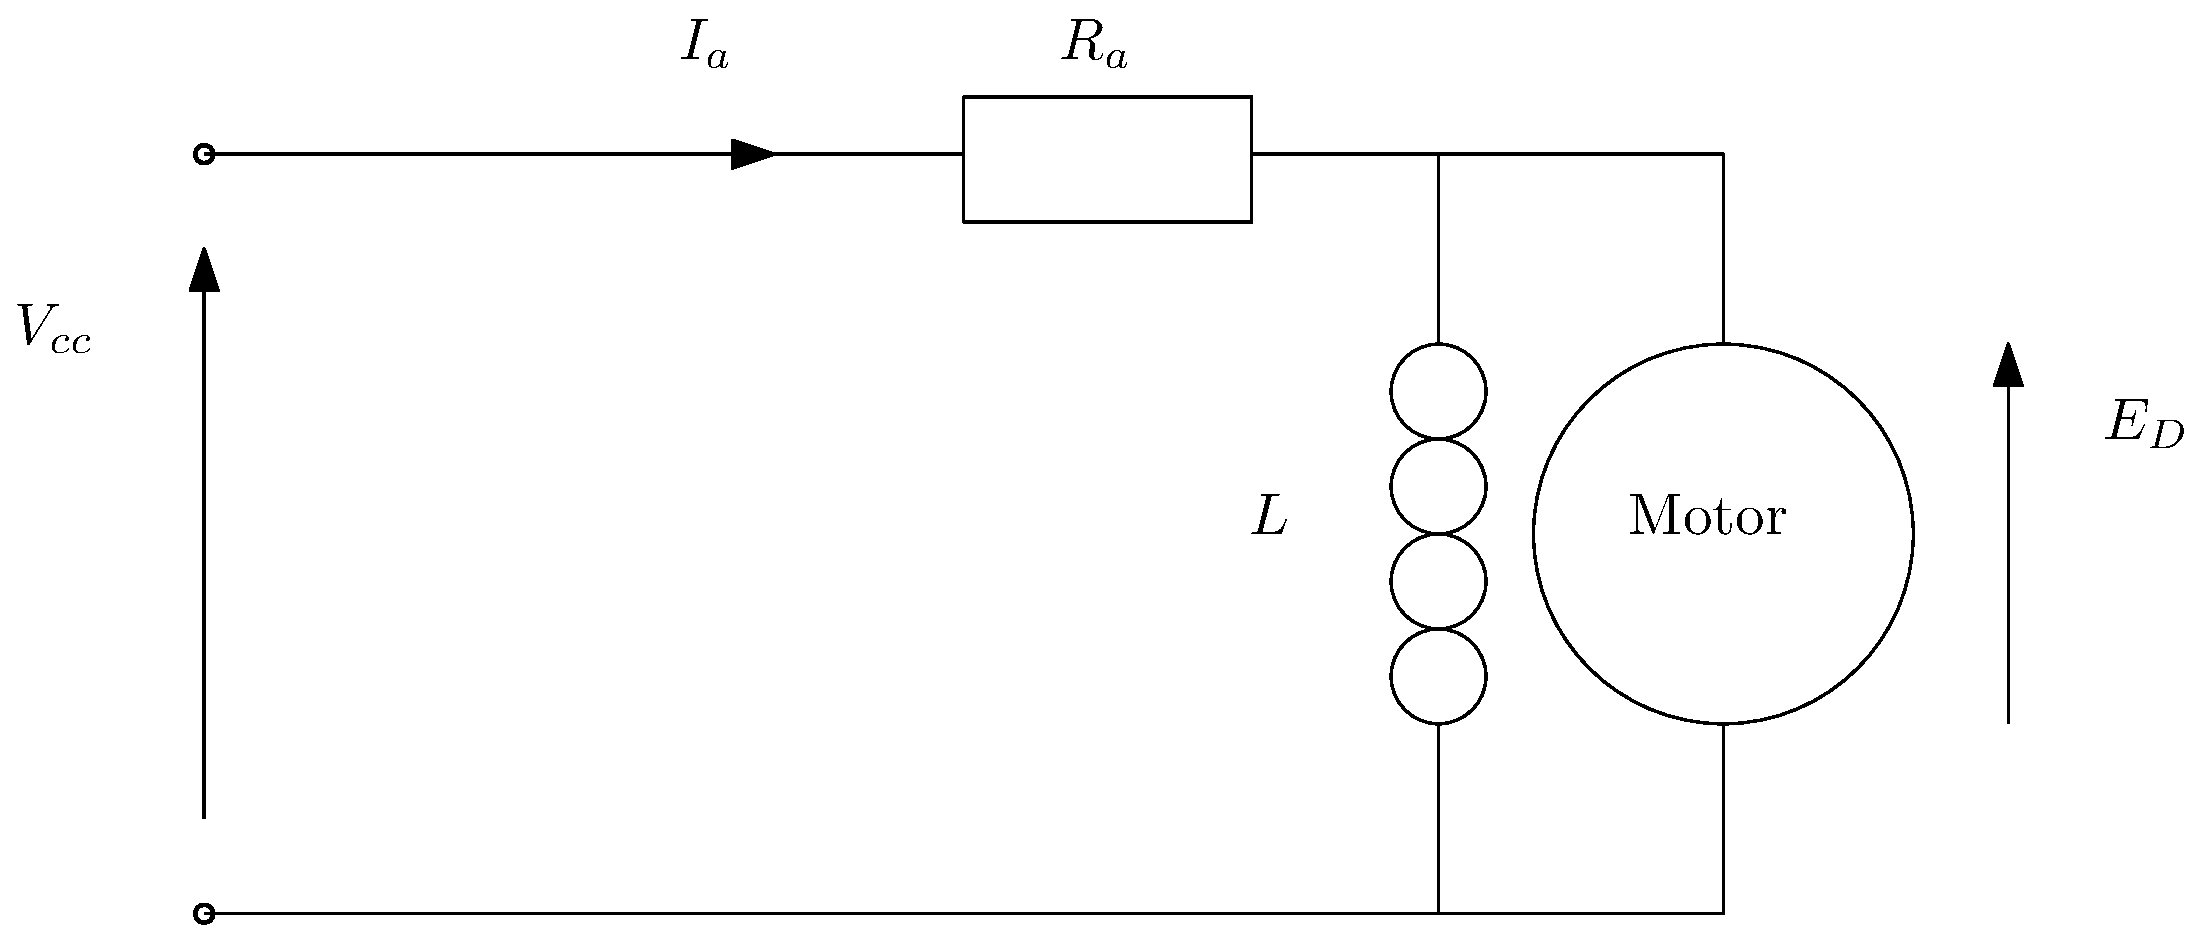
\includegraphics[width=0.9\linewidth]{dc_circuit.eps}
	\caption{Steady state equivalent circuit for a DC motor.}
	\label{fig:dc_circuit}
\end{figure}

This simple circuit leads to the relationship between current and internal resistance given by Equation \ref{eq:steady_state}.
\begin{equation}
	V_{cc} = E_D + I_a R_a
	\label{eq:steady_state}
\end{equation} 
It should be noted that the brushless DC motor is sometimes grouped with AC machines such as the induction motor due to its varying excitation \cite{Sarlioglu2016}. The coils are energised in order to keep the magnetic field at 90 degrees to the field generated by the permanent magnets mounted on the rotor. 

The field strength of the magnets, the number of poles and the number turns of the armature coils can be captured in the motor constant $k_T $ relating torque to armature current.

\begin{equation}
	\tau = k_T I_a
	\label{eq:torque_constant}
\end{equation} 

\begin{equation}
	E_D = \frac{rpm}{k_e}
	\label{eq:emf_constant}
\end{equation} \\

There are numerous loss sources in an electric motor such as winding resistance, flux leakage, eddy currents in the core and so on \cite{Sarlioglu2016}. By using real-world measured mechanical power output and electrical input, an equivalent winding resistance $R_a$ for the simple model can be found. The parameters are shown in Table \ref{tab:motor_params}. 

\begin{table}
	\caption{Motor parameters used in simulation.}
	\label{tab:motor_params} 
	\centering
	\begin{tabular}{ |c|c| }
		\hline
		$k_v$ [rpm/v]& 6 \\ 
		$k_T$ [Nm/A] & 1.53 \\ 
		$P_{mech}$@375rpm [kW] & 3.6 \\ 
		$P_{elec}$@375rpm [kW]& 6.37 \\
		*$R_a$ [Ohms] & 1.0 \\
		\hline
	\end{tabular}
\end{table}

\subsection{Air Resistance}
In addition to the resistive losses in the motor windings losses due to air resistance were also modelled. AGVs  typically operate at low speed <3m/s, hence the unaerodynamic shape of many models. However, the target speed of 10m/s is quite high around 30 miles per hour and drag could become significant. 

The drag coefficient $C_{drag}$=1 for a cuboid shape was used, taken from \cite{Toolbox2004}. The frontal area $A$ of 1m$^2$ is consistent with a box shape for maximum load carrying capacity. The density of air at room temperature is close to 1kg/m$^3$.

\begin{equation}
	F_D = C_{drag} \rho v^2 A
\end{equation} 


\subsection{Arrival Distribution}
%*see Arrival Distribution for Intersection Simulation (Sources!).docx
Previous work in road traffic modelling has used a variety of point distributions to model arrivals. A good summary is given in \cite{Knoop2020} or the chapter on Microsimulation in \cite{Sheffi1985}. 

\subsubsection{Learning from Road Transport Models}
\begin{figure}
	\centering
	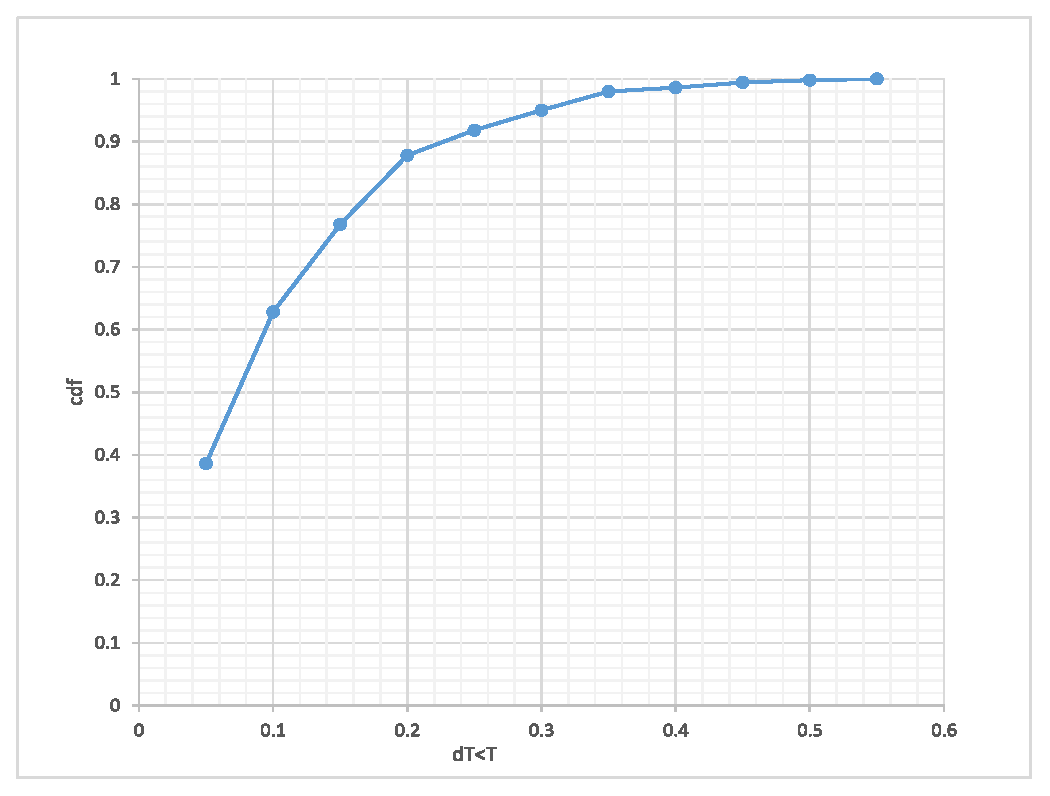
\includegraphics[width=0.9\linewidth]{poisson_cdf.eps}
	\caption{Cumulative Distribution Function of arrivals following a Poisson distribution.}
	\label{fig:poisson_cdf}
\end{figure}
One option is to assume arrivals at a point are completely independent of each other, but occur at an average rate for the time of day which has been measured by inductive loop placed in the road. These assumptions lead to a Poisson distribution such as that shown in Figure \ref{fig:poisson_cdf}. This can be generated computationally by drawing a sequence of numbers from a uniform distribution and applying Equation \ref{eq:poisson_delta} to compute the time delta until the next arrival. To validate the arrivals drawn in this way, we check the log plot of the frequency against time delta is linear and the median is equal to the specified rate as shown in Figure \ref{fig:1_minus_ln_cdf_arr}.   
\begin{figure}
	\centering
	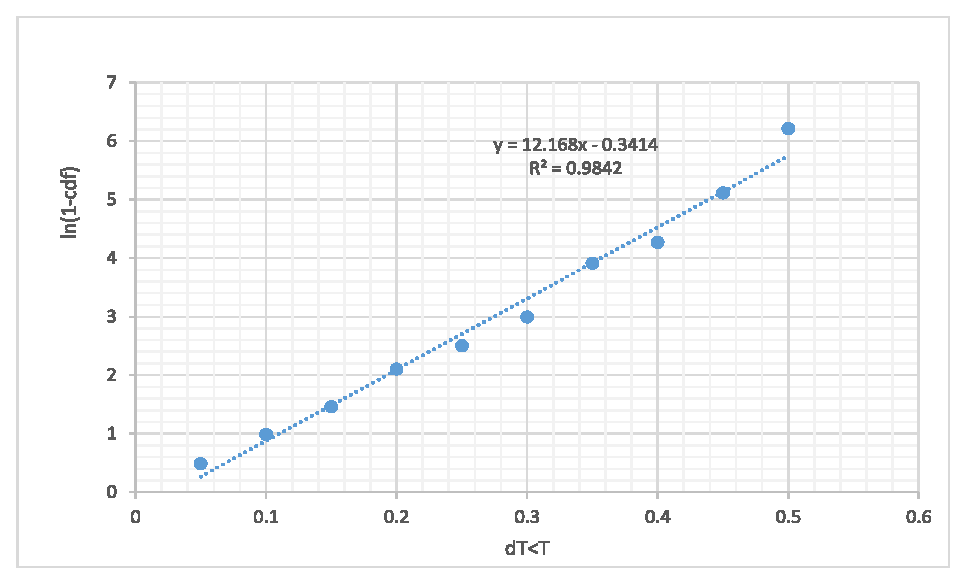
\includegraphics[width=0.9\linewidth]{ln(1-cdf)poisson_arr.eps}
	\caption{Log Cumulative Distribution Function of arrivals with linear fit.}
	\label{fig:1_minus_ln_cdf_arr}
\end{figure}


The assumption that arrivals are independent does not hold if traffic density is high. This is because vehicles slow down to keep a safe distance from the one in front of them. The simplest modification to the poisson distribution to account for this is to discard time deltas which violate the specified safe headway, leading to the shifted exponential distribution. A scatter plot of times from this distribution is shown in Figure \ref{fig:poisson_shifted_scatter}. Now the arrivals will always be realistic in the sense vehicle will not overlap/arrive unsafely but the variance will be smaller. The two parameters the average arrival rate $\lambda$ and the minimum safe headway $\tau$ together control the variance. This is because the median of the distribution must be $\lambda$, so if $1/\tau$ is close to $\lambda$ the variance must be very small.   

\begin{figure}
	\centering
	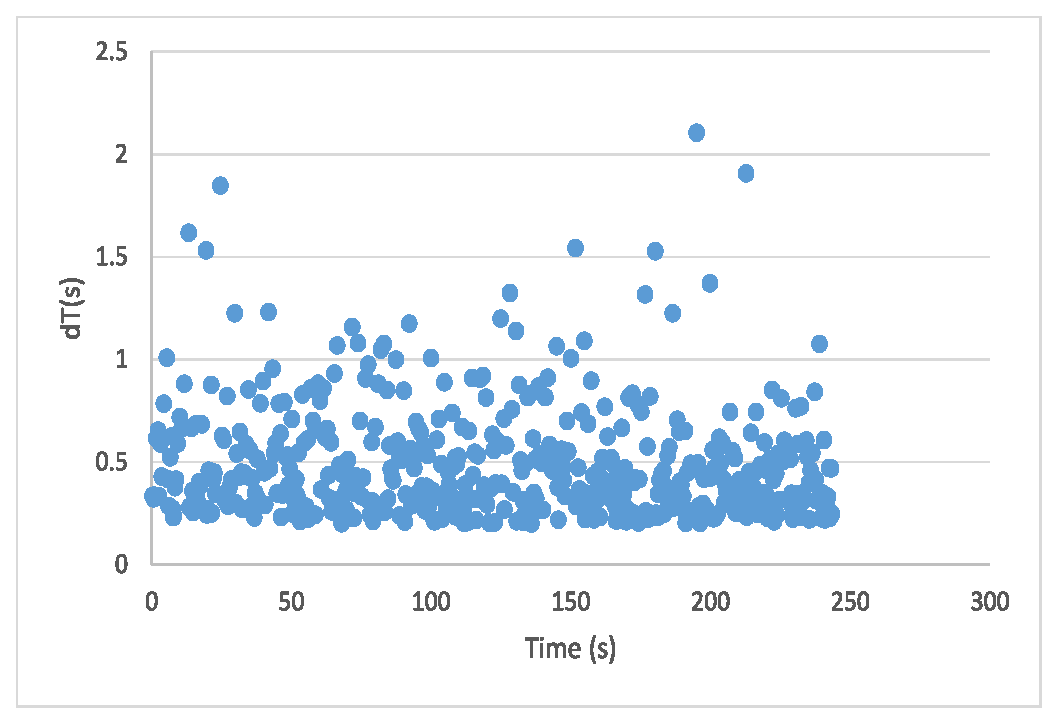
\includegraphics[width=0.9\linewidth]{poisson_shifted_scatter.eps}
	\caption{Scatter plot of 500 arrival time deltas drawn from a shifted exponential distribution with a minimum headway of 0.2 seconds.}
	\label{fig:poisson_shifted_scatter}
\end{figure}
\begin{figure}
	\centering
	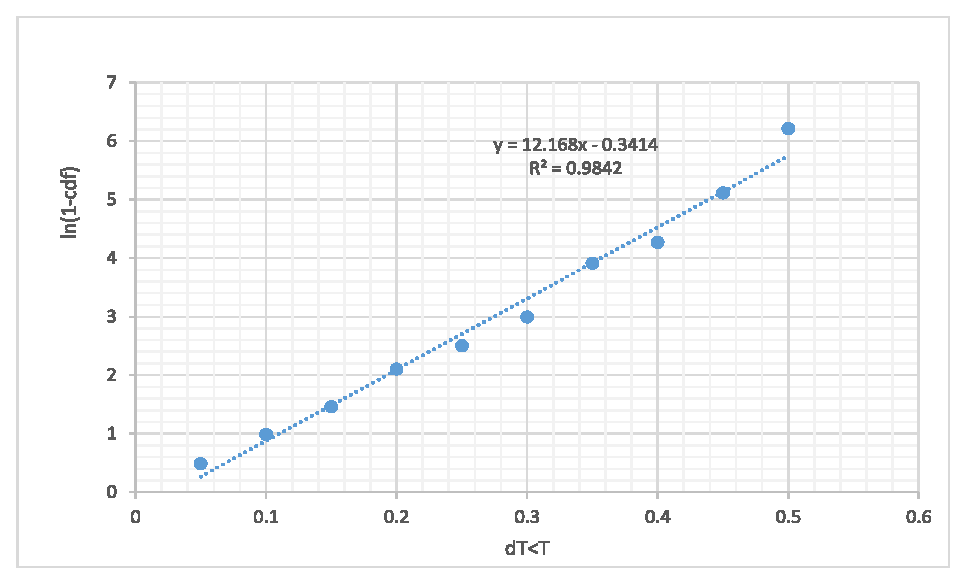
\includegraphics[width=0.9\linewidth]{ln(1-cdf)poisson_arr.eps}
	\caption{Log Cumulative Distribution Function of arrivals with linear fit.}
	\label{fig:1_minus_ln_cdf_arr}
\end{figure}

\subsubsection{Unique Features of AGV Traffic}
The arrival distribution corresponds to the properties of AGV traffic satisfying the following assumptions:
\begin{itemize} 
	\item{More than one AGV is permitted to enter the same link if they are travelling in the same direction.}
	\item{Entry to links in the roadmap is denied if the number already present on the link reaches a fixed capacity}
	\item{Car-following behaviour within the link is governed by the frontal safety system on board each AGV. This provides an outer (warning) zone which, if tripped, the AGV will slow to $w$m/s at $a_w$m/s and an inner zone (emergency)), which if tripped the vehicle will come to a complete stop at $a_e$m/s, where $|a_e|$ > $|a_w|$}
	\item{The capacity of a link is the number of AGVs which would fit without the inner front safety zone of each being tripped by the one in front. This can be calculated for $n$ AGVs each with safety zone length $d_e$ as $n_c = n\dot d_w$}
	\item{Every AGV is informed whether it is able to proceed before it reaches the end of its current link. The AGV will keep slowing down to stop at the end, until it is informed there is space on the next link, at which point it will accelerate to full speed. }
\end{itemize}

According to these assumptions, a suitable model is the shifted exponential, with a minimum headway based on the size of the AGV safety zone. 

\subsubsection{Arrival Variation Based on Approach Lane Occupancy}
Another consideration is how the traffic on the approach lanes should feed back into the arrival times. Based on the counting semaphore for each link assumption, this can be modelled with two queues at the entryway. The lane queue and the busy queue. If the occupancy of the lane is less the $n_c$, new arrivals are added to the lane queue at full speed, in the simulation interval exceeding their point arrival time, at a position they would have reached by the simulation time. If the occupancy of the lane is more than $n_c$ new arrivals are added to the back of the busy queue. At the next time step where $n<n_c$, the AGV at the front of the busy queue is moved onto the lane. The arrival speed is reduced according to acceleration rate $a_W$ based on the time between the arrival and the time step where is can proceed. For longer time periods the new arrival will have zero speed. All arrivals which were not at the front of the busy queue will arrive at the warning speed $v_w$=0.3m/s. 


\subsection{Division of Responsibility Between Intersection and AGV Controllers}
With different signal-free intersection control approaches, the functionality carried out centrally by the fixed-server compared to that by the mobile AGV varies significantly. Of particular interest are the interfaces used by Digani et al \cite{Digani2019} where the intersection provides average speeds for discrete segments, and the one used by Levin and Rey \cite{Levin2017} where the reservation message sent by the intersection contains the arrival time at the conflict point. 

The arrival time at the conflict point is similar to a widely used waypoint interface. As the time is the important quantity for ensuring collisions are avoided this interface seems more sensible. However, on its own it is not sufficient to ensure FIFO behaviour of AGVS approaching in the same lane. Many studies assume an external mechanism for car-following based on local sensors such as the Intelligent Driver Model in \cite{He2020}.  

Without a car-following or platooning approach locally on the AGV, simple methods to manage cross traffic can easily fail to maintain FIFO ordering. This problem is often encountered in traffic simulation with cellular models and there are various techniques to avoid it without generating a trajectory for each vehicle \cite{Carey2014}. 

\cite{Levin2017} and \cite{Digani2019} do not mention any local car following behaviour and seek to avoid all collisions by the centralised application of constraints. This makes it difficult to compare them to a semaphore based intersection controller, unless car following is used in combination with semaphore access control.  

\section{Methods For Zone-Based Intersection}
\subsection{Intersection Controller Objective}
The objective is to minimize $J_T$ the total travel time for all vehicles. It is convenient for exposition to optimize over the inverse of speed of each segment $\phi_k = 1/v_k$. Vehicle $i$ submits a plan containing $m_i$ segments before the conflict and $n_i$ segments in conflict. The control model is based on the average speed of each approaching AGV over each segment. This is to simplify the description of the intersection controller, and assist analysis. More sophisticated motion models could take the place of  Equation \ref{eq:omega_min} and  Equation \ref{eq:omega_max} to create a similar type of problem with a convex travel time objective and non-convex constraints.   
The parameters for one vehicle can be collected in the vector $\bm{\phi}_i$ as shown in Equation \ref{eq:phi_i}
\begin{equation}
	\bm{\phi}_i =  [\phi_{1}, ..., \phi_{(m_i + n_i)}]^T \\
	\label{eq:phi_i}
\end{equation}
The parameters for $p$ vehicles each traversing $(m_i + n_i)$ segments are assembled into a vector as in Equation \ref{eq:parameters}
\begin{equation}
	\bm{\phi} = [\bm{\phi_{1}}^T, ..., \bm{\phi}_{p}^T]^T \\
	\label{eq:parameters}
\end{equation}
Similarly, the length of each segment in plan $i$ can be arranged into a vector 
\begin{equation}
	\bm{d}_i = [d_{1}, ..., d_{(m_i + n_i)}]^T \\
	\label{eq:d_i}
\end{equation}
and collected  for $p$ vehicles into a vector as in Equation \ref{eq:d}.
\begin{equation}
	\bm{d} = [\bm{d_{1}}^T, ..., \bm{d}_{p}^T]^T \\
	\label{eq:d}
\end{equation}
This leads to the minimum travel time objective in Equation \ref{eq:qp_speeds}. 
\begin{equation}
	\begin{array}{c}
		\min \limits_{\bm{\phi}} \bm{J_T} = \bm{d}^T \bm{\phi} \\
		\textrm{subject to}\\
		\bm{\phi}_{max} > \bm{\phi} > \bm{\phi}_{min} \\
		\bm{\phi}^T\bm{H}_{i,j}\bm{\phi} > \bm{0} \quad \forall i,j \in [1,p] \quad \textrm{with } j>i \\
	\end{array}
	\label{eq:qp_speeds}
\end{equation}

The condition $j>i$ in Equation \ref{eq:qp_speeds} indicates that the number of constraints varies with the number of vehicles $p$ as $\frac{p(p-1)}{2}$. This corresponds to one constraint between each pair of approaching AGVs.

\subsection{Intersection Controller Timing Constraints}
By definition, each intersection has a single conflict zone, the union of all segments which intersect there. This makes it possible to express the constraint that vehicles do not collide in terms of time. Vehicle $i$ arrives at the first conflicted segment $\omega_i^{min}$ and departs from the last at $\omega_i^{max}$. The following three subsections set out three alternative ways of expressing the collision avoidance constraints which have been evaluated. 
The arrival time is given by Equation \ref{eq:omega_min}. Considering average speeds, the departure time $\omega_i^{max}$ is also linear, this is given by Equation \ref{eq:omega_max}. 
\begin{equation}
	\omega_i^{min}  = \sum_{k=1}^{m_i} \bm{d}_i [k] \bm{\phi}_i [k] = \bm{e}^T \bm{\phi}_i
	\label{eq:omega_min}
\end{equation}
where %$\bm{e}[k] = \bm{d}_i[k] \forall k <m_i, otherwise 0$
\begin{equation}
	\bm{e}[k] = \left\{
	\begin{array}{cc}
		\bm{d_i}[k] & \forall k <m_i \\
		0 & \textrm{otherwise} \\
	\end{array}
	\right.
\end{equation}  and $m_i$ is the number of segments on the path of vehicle $i$ before arrival at the conflicted segment. 
\begin{equation}
	\omega_i^{max}  = \omega_i^{min} + \sum_{i=1}^{n_i} \bm{d}_i [k] \bm{\phi}_i [k] = \bm{f}^T \bm{\phi}_i
	\label{eq:omega_max}
\end{equation}
where 
\begin{equation}
	\bm{f}[k] = \left\{
	\begin{array}{cc}
		\bm{d_i}[k] & \forall k <m_i+n_i \\
		0 & \textrm{otherwise} 
	\end{array}
	\right.
\end{equation}
and $n_i$ is the number of segments on the path of vehicle $i$ which are conflicted. Note that Equations \ref{eq:omega_min} and \ref{eq:omega_max} only depend on the $\bm{\phi}_i$ of vehicle $i$. 



\subsubsection{Linear FIFO Constraints}
\label{sec:fifo_constraints}
If the order in which the AGV cross the conflict zone is fixed to be First-In-First-Out, the timing constraint is linear. For a pair where the leader enters the conflict at $t_i$ and takes $\Delta t_i$ seconds to cross at maximum speed the condition for entry time of the follower $t_{i+1}$ given by Equation \ref{eq:entry_time}.

\begin{equation}
	-t_{i} + t_{i+1}	\leq	\Delta t_i
	\label{eq:entry_time} 
\end{equation} 

There is one constraint between each adjacent pair so $p-1$ constraints total for $p$ vehicles. These can be expressed in the form $\bm{A}_{ub}\phi \leq \bm{b}_{ub}$ as in Equation \ref{eq:fifo}. This is correct for two AGV arranged in distance order, each traversing one approach and one conflict segment. 



\begin{equation}
	\left[ 
	\begin{array}{ccccc}
		-d_1 & d_2 & \bm{0}\\
		\vdots & \ddots & \vdots \\
		\bm{0} & -d_{p-1} & d_p\
	\end{array} \right]
	\left[
	\begin{array}{c}
		\phi_1 \\ \vdots \\ \phi_p
	\end{array} \right]
	\leq
	\left[ 
	\begin{array}{c}
		\Delta t_1 \\
		\vdots \\
		\Delta t_{p-1}
	\end{array} \right]
	\label{eq:fifo}
\end{equation}

The timing constraint between each pair of vehicles can be expressed with a modulus operator as in Equation\ref{eq:timing}.
\begin{equation}
	|\alpha_i - \alpha_j| > \beta_i + \beta_j
	\label{eq:timing}
\end{equation}

Here 
\begin{equation}
	\alpha_i  = \omega_i^{max} + \omega_i^{min}
	\label{eq:alpha}
\end{equation}
represents the midpoint of the time vehicle $i$ occupies the conflicted segment and
\begin{equation}
	\beta_i  = \omega_i^{max} - \omega_i^{min}
	\label{eq:beta}
\end{equation}
represents the range of the time either side of the midpoint, both scaled by a factor of two. 


In matrix form
\begin{equation}
	\alpha_i  = \bm{f}^T \bm{\phi}_i + \bm{e}^T \bm{\phi}_i = \bm{1}_i^T\bm{A}{\phi}_i
	\label{eq:alpha_m}
\end{equation}
with $\bm{A} = diag(\bm{f} + \bm{e})$
\begin{equation}
	\beta_i  = \bm{f}^T \bm{\phi}_i - \bm{e}^T \bm{\phi}_i =  \bm{1}_i^T\bm{B}{\phi}_i
	\label{eq:beta_m}
\end{equation}
with $\bm{B} = diag(\bm{f} - \bm{e})$

The resulting linear program (with parameters $\in\mathbb{R}$) has $p-1$ constraints as each AGV is only constrained by the preceding one.

\subsubsection{Quadratic Constraints}
\label{sec:quad_constraints}
Another way to treat the modulus operator in Equation \ref{eq:timing}, without forcing any particular arrival order is to square both sides as to give the expression in Equation \ref{eq:expanded}. 
\begin{equation}
	\alpha_i^2 - \alpha_j^2 - 2 \alpha_i\alpha_j - (\beta_i^2 + \beta_j^2 +2 \beta_i \beta_j) > 0
	\label{eq:expanded}
\end{equation}
Collecting terms by subscript gives
\begin{equation}
	(\alpha_i^2 - \beta_i^2) - (\alpha_j^2 + \beta_j^2) - 2(\alpha_i\alpha_j + \beta_i \beta_j) > 0
	\label{eq:collected}
\end{equation}

The matrix $\bm{\Lambda}_ij$ captures the constraints between a pair of vehicles and always contains four sub-matrices as shown in in Equation \ref{eq:lambda}. It is compatible with $\bm{\phi}_{i,j} = [\bm{\phi}_i^T, \bm{\phi}_j^T]^T$, containing only the relevant speeds for vehicles $i$ and $j$. 
\begin{equation}
	\bm{\Lambda}_{ij} =\left[
	\begin{array}{cc}
		\bm{\Lambda}_{ij}^{ii} & \bm{\Lambda}_{ij}^{ij} \\
		\bm{\Lambda}_{ij}^{ji} & \bm{\Lambda}_{ij}^{jj} \\
	\end{array}
	\right]
	\label{eq:lambda}
\end{equation}
Expanding 
\begin{multline}
	\left[\bm{\phi}_i^T, \bm{\phi}_j^T\right]
	\left[\begin{array}{cc}
		\bm{\Lambda}_{ij}^{ii} & \bm{\Lambda}_{ij}^{ij} \\
		\bm{\Lambda}_{ij}^{ji} & \bm{\Lambda}_{ij}^{jj} \\
	\end{array}\right]
	\left[\begin{array}{c}
		\bm{\phi}_i\\
		\bm{\phi}_j \end{array} \right] \\
	= \bm{\phi}_{i}^T \bm{\Lambda}_{ij}^{ii} \bm{\phi}_{i} + \bm{\phi}_{j}^T \bm{\Lambda}_{ij}^{jj} \bm{\phi}_{j} + \bm{\phi}_{i}^T \bm{\Lambda}_{ij}^{ij} \bm{\phi}_{j} + \bm{\phi}_{j}^T \bm{\Lambda}_{ij}^{ji} \bm{\phi}_{i}
\end{multline}
makes it possible to compare terms with the scalar expression in Equation \ref{eq:collected}. This leads to the following expressions for the submatrices in $\Lambda$ in terms of $\alpha_i = \bm{1}_T\bm{A}_i\bm{\phi}_i$ and $\beta_i = \bm{1}_T\bm{B}_i\bm{\phi}_i$ 
\begin{equation}
	\bm{\Lambda}_{ij}^{ii} = (\bm{A}_i - \bm{B}_i)\bm{1}_i\bm{1}_i^T(\bm{A}_i - \bm{B}_i) 
	\label{eq:ii}
\end{equation}
\begin{equation}
	\bm{\Lambda}_{ij}^{jj} = -(\bm{A}_j + \bm{B}_j)\bm{1}_j\bm{1}_j^T(\bm{A}_J + \bm{B}_j) 
	\label{eq:jj}
\end{equation}
\begin{equation}
	\bm{\Lambda}_{ij}^{ij} + \bm{\Lambda}_{ij}^{ij T} = -2(\bm{A}_j + \bm{B}_j)\bm{1}_j\bm{1}_i^T(\bm{A}_i + \bm{B}_i) 
	\label{eq:ij}
\end{equation}

For more than two vehicles this can be arranged into a block diagonal matrix $\bm{H}_{ij}$ which is compatible with the input parameters, but still only represents the constraints between a pair. 

Expressed in this way it is clear the constraints are quadratic and it is trivial to differentiate twice to find the Hessian is the stack of constraint matrices $[\bm{H}_{ij}, \hdots]$. The objective is certainly convex as it is linear but the constraints may not be. If the Hessian of the constraints is positive semi-definite then they are convex and interior point methods will either find the global optimum or prove that there is no feasible solution \cite{Boyd2004}. The Hessian depends on the parameters of the roadmap, the number of approaching vehicles and their distance from the conflict. 

\subsubsection{Mixed Integer Constraints}
\label{sec:milp_constraints}
A third way of treating the timing constraint in Equation \ref{eq:timing}, also without forcing any particular arrival order involves splitting each constraint into two based on the sign of $(\alpha_i-\alpha_j)$ as shown in equation \ref{eq:or_cons}. Again, this is expressed in terms of the midpoint $\alpha_i$, $\alpha_j$ and extent $\beta_i$,$\beta_j$ of the time when vehicle $i$ and vehicle $j$ occupy the segment on their own path which passes through the conflict point,
\begin{equation}
	\begin{array}{cc}
		\alpha_i - \alpha_j > \beta_i + \beta_j &\textrm{if  }\alpha_i >\alpha_j  \\
		\alpha_i - \alpha_j < -(\beta_i + \beta_j) & \textrm{otherwise}\\
		\textrm{where } \alpha_i, \alpha_j, \beta_i, \beta_j >0
	\end{array}
	\label{eq:or_cons}
\end{equation}
In order to apply these OR constraints, an additional integer parameter $b_k$ can be introduced for each pair of AGV, along with an arbitrary large number $M$ as shown in Equation \ref{eq:big_m_cons}. 
\begin{equation}
	\begin{array}{cc}
		\alpha_i - \alpha_j + b_{i,j}M > \beta_i + \beta_j \\
		\alpha_i - \alpha_j - (1-b_{i,j})M < -(\beta_i + \beta_j) \\
		\textrm{where } b_{i,j}\in[0,1] \\
		M>>\alpha_i, \alpha_j, \beta_i, \beta_j
	\end{array}
	\label{eq:big_m_cons}
\end{equation}
Now the problem is combinatorial rather than convex and appropriate methods must be used. These may be based on exhaustive search such as Branch-and-Bound, or solving a sequence of convex relaxations of the original problem \cite{Murray2010}. Combinatorial problems quickly become intractable for large numbers of variables, but in this case the underlying problem of arrival order is combinatorial, so exhaustive methods are needed to find the global minimum. 

It is possible to further assume every AGV travels at maximum speed once it reaches the conflict, simplifying equation Equations \ref{eq:alpha} and \ref{eq:beta} with a constant $p_i = g_i \phi_{min}$. 
\begin{equation}
	\alpha_i = 2\omega_i^{min} + p_i
\end{equation}
\begin{equation}
	\beta_i = p_i
\end{equation}
where $g_i$ is the length of the conflicted segments in the plan of vehicle $i$. In this case Equation \ref{eq:big_m_cons} can be restated 
\begin{equation}
	\begin{array}{cc}
		\omega_i^{min} - \omega_j^{min} + b_{i,j}M > p_j \\
		\omega_i^{min} - \omega_j^{min}  - (1-b_{i,j})M < -p_i \\
		\textrm{where } b_{i,j}\in[0,1] \\
	\end{array}
	\label{eq:minlp}
\end{equation}

\section{Methods For Conflict Point Intersection}
For a intersection between roads with multiple lanes, it makes sense to plot the centreline of each lane, and the arc of each turning motion between lanes. Any point where two of these arcs cross is called a conflict point. By controlling arrival time at a conflict point, collisions can be avoided, while vehicles that do not pass the same conflict point can both proceed \cite{Levin2017}.

\begin{figure}[ht]
	\centering
	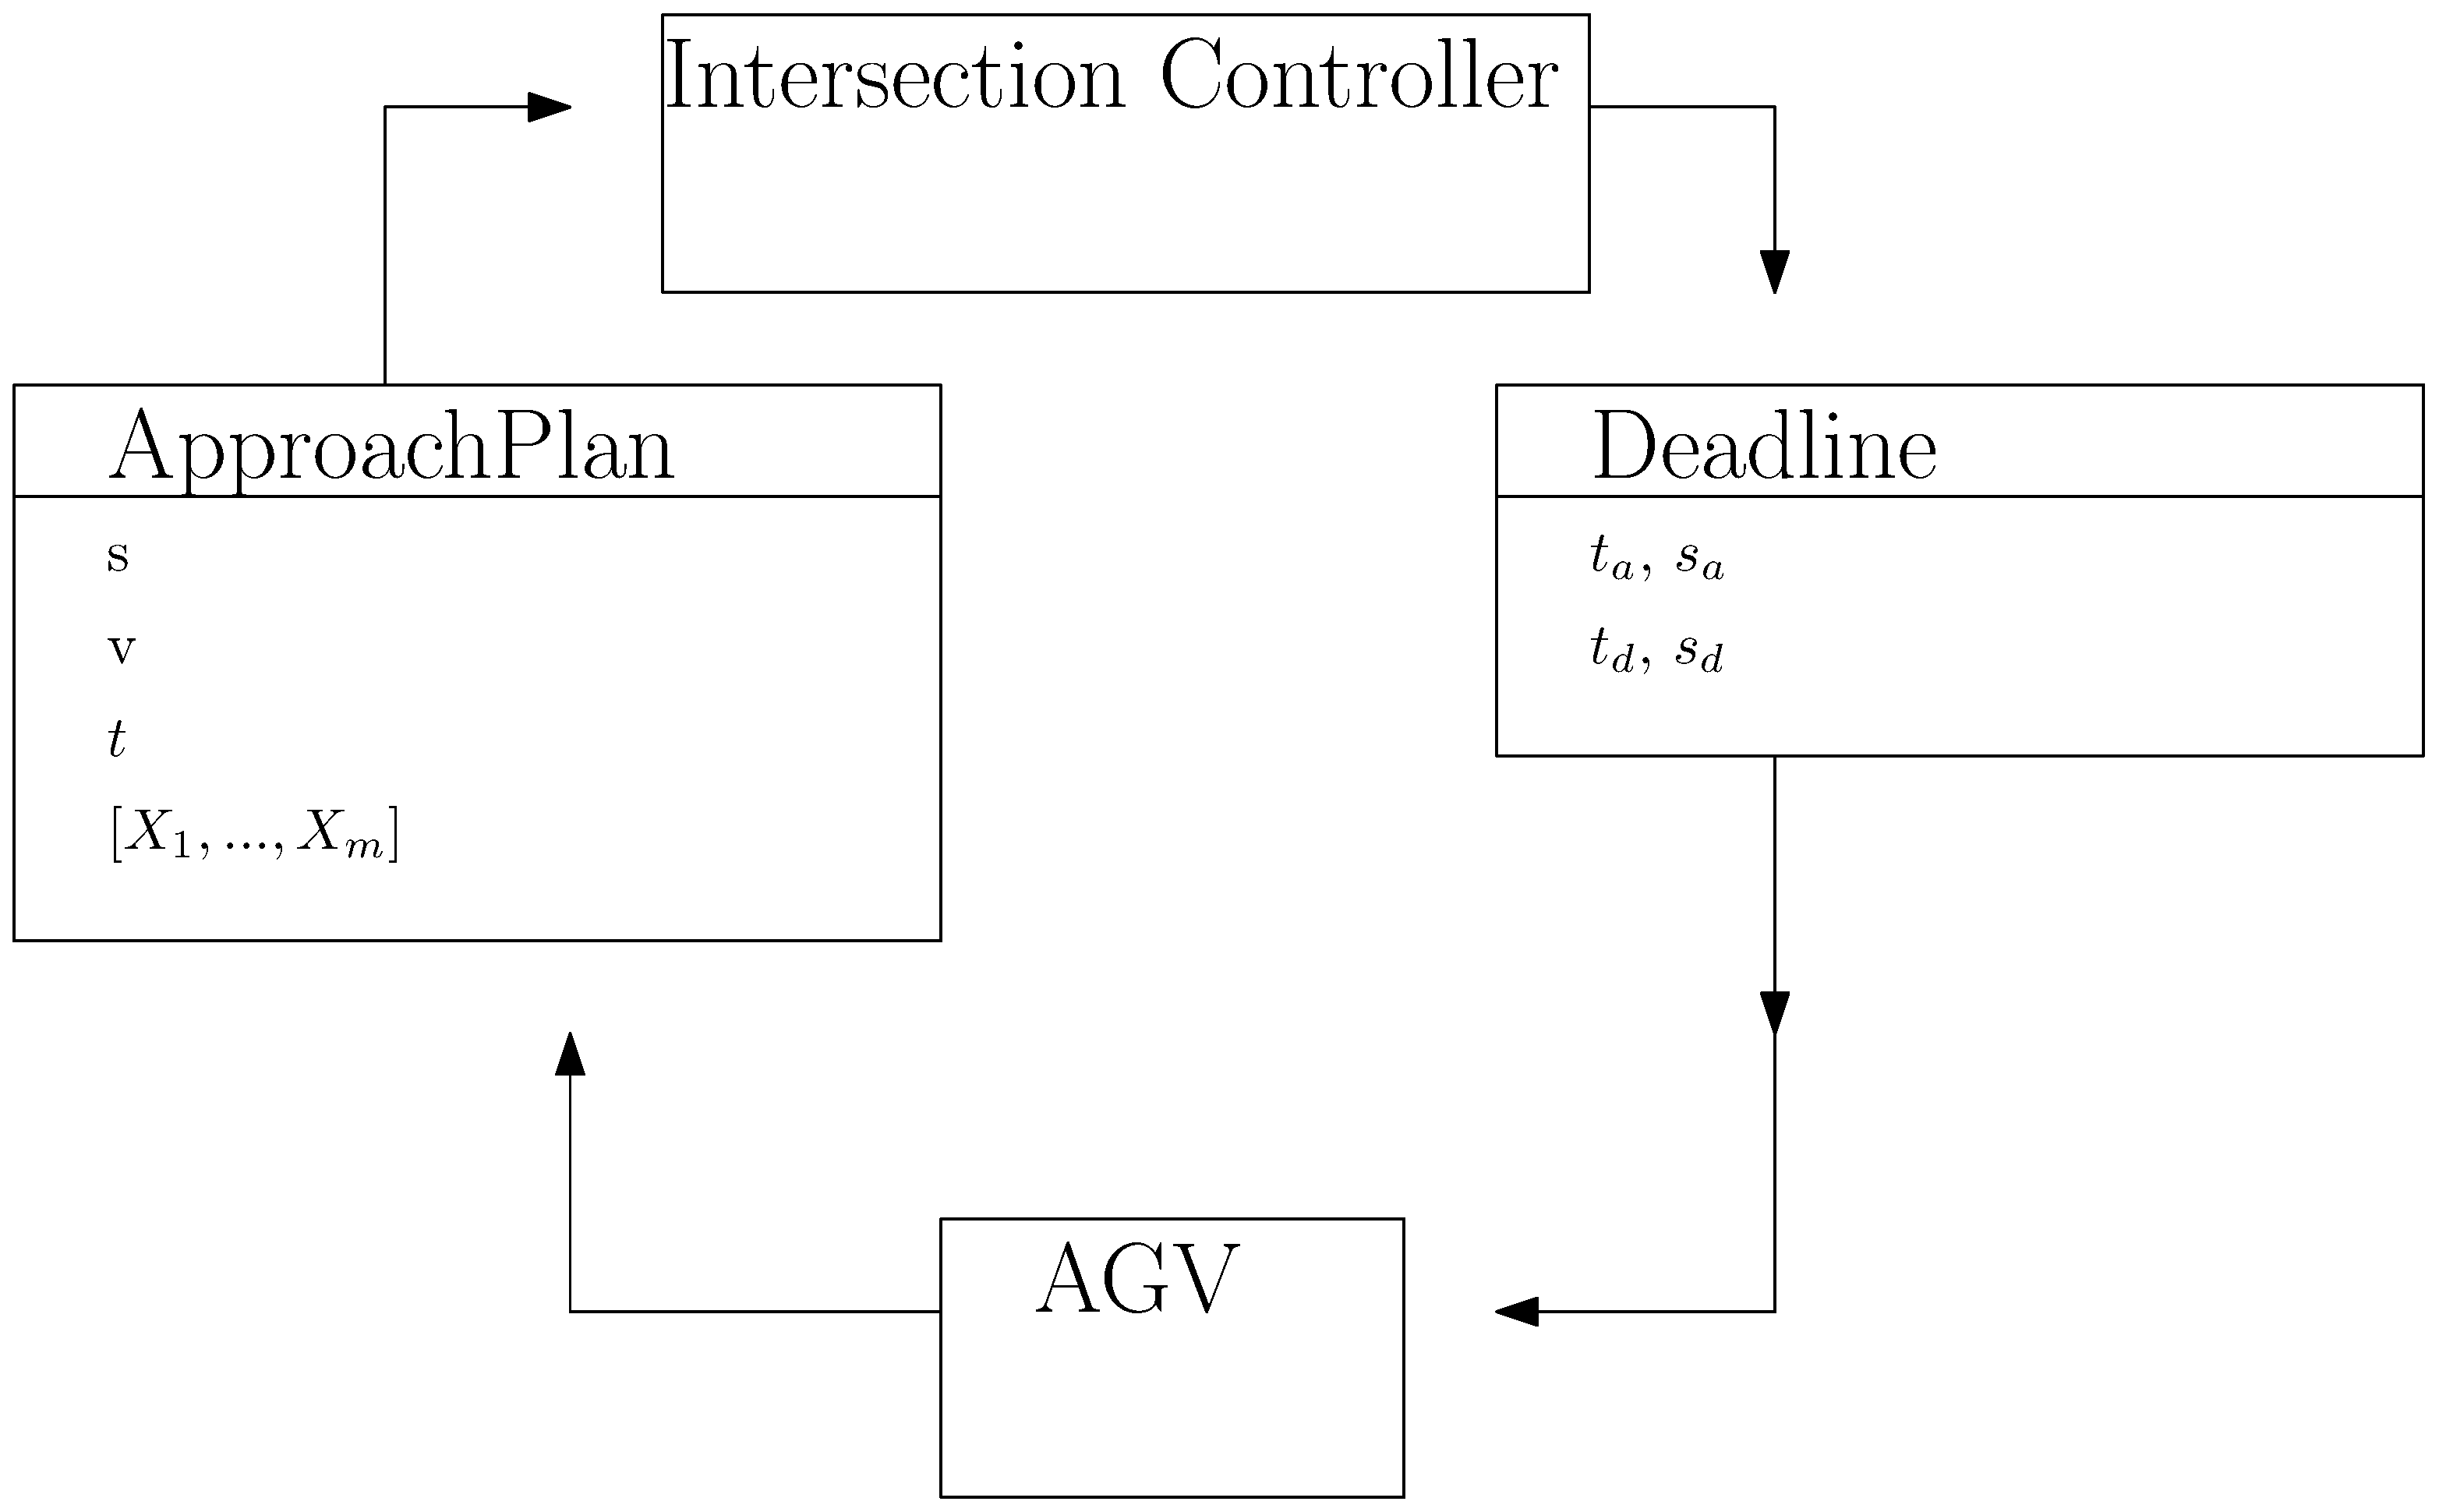
\includegraphics[width=0.9\linewidth]{plan_deadline_interface.eps}
	\caption{Key messages of the ``Plan/Deadline'' interface governing access to a conflict point intersection.}
	\label{fig:plan_deadline_interface}
\end{figure}

A controller based on a common heuristic for controlling access to a shared resource, the binary semaphore, is included for comparison with the optimal methods.  Similar approaches are widespread in AGV control \cite{Duinkerken1999} and \cite{Lee2019}.


\subsection{Semaphore Approach}
To implement the ``plan/deadline'' interface, a binary semaphore for each conflict point was needed. The semaphore controller does not compute the entry and exit times of the conflict as it has is no model of the vehicle dynamics. It simply raises the semaphore, sending a ``full speed ahead'' message to the closest AGV to the intersection and a position deadline to all others.

For this reason the deadline message contains the position at which the agv must stop, without any timing. The AGV must stop at the given position until it receives a 'proceed' message form the intersection controller.

\section{Performance Comparison}
Both conflict point representation and the zone representation are identical if the intersection has exactly one conflict. On this basis the semaphore approach and two versions of minimum crossing time optimal control, one with FIFO linear constraints and the other with quadratic constraints were compared on a simulated intersection comprising two lanes which cross in the middle. The approach distance is fixed at 15 metres.

The controllers will be tested with traffic levels and control latencies intended to bound the likely values of these parameters, shown in Table \ref{tab:test_params}.

\begin{table}
	\caption{Parameters bounds used to generate test scenarios.}
	\label{tab:test_params} 
	\centering
	\begin{tabular}{ |c|c|c| }
		\hline
		Parameter & High Bound & Low Bound \\
		$T_C$ [s]& 0.5 & 0.1 \\ 
		$\frac{1}{\lambda}=\Delta T_a$ [s]& 10 & 2 \\ 	
		\hline
	\end{tabular}
\end{table}

\begin{table}
	\begin{tabular}{|c|c|c|c|}
		\hline
		& $\lambda_1$ & $\lambda_2$ & $f$ \\
		\hline
		HLHT & 0.5 & 0.5 & 2 \\
		HLMT & 0.1 & 0.5 & 2 \\
		HLLT & 0.1 & 0.1 & 2 \\
		LLHT & 0.5 & 0.5 & 10 \\
		LLMT & 0.1 & 0.5 & 10 \\
		LLLT & 0.1 & 0.1 & 10 \\
		\hline
	\end{tabular}
	\label{tab:params}
	\caption{Parameters for test scenarios. All units s$^-1$. Each scenario is identified with the first two characters relating to the latency between periodic messages from the intersection controller where High Latency is 500ms and  Low Latency is 100ms and the second two relating to the arrival rate, where High Traffic has $\lambda$=10 arrivals per second on both approaches, Low Traffic has $\lambda$=2 arrivals per second on both, and Mixed Traffic has one lane with $\lambda_1$=10 and the other with $\lambda_2$=2. For example High Latency, High Traffic becomes HLHT.}
\end{table}

\section{Simulation Results}

\begin{figure}[ht]
	\centering
	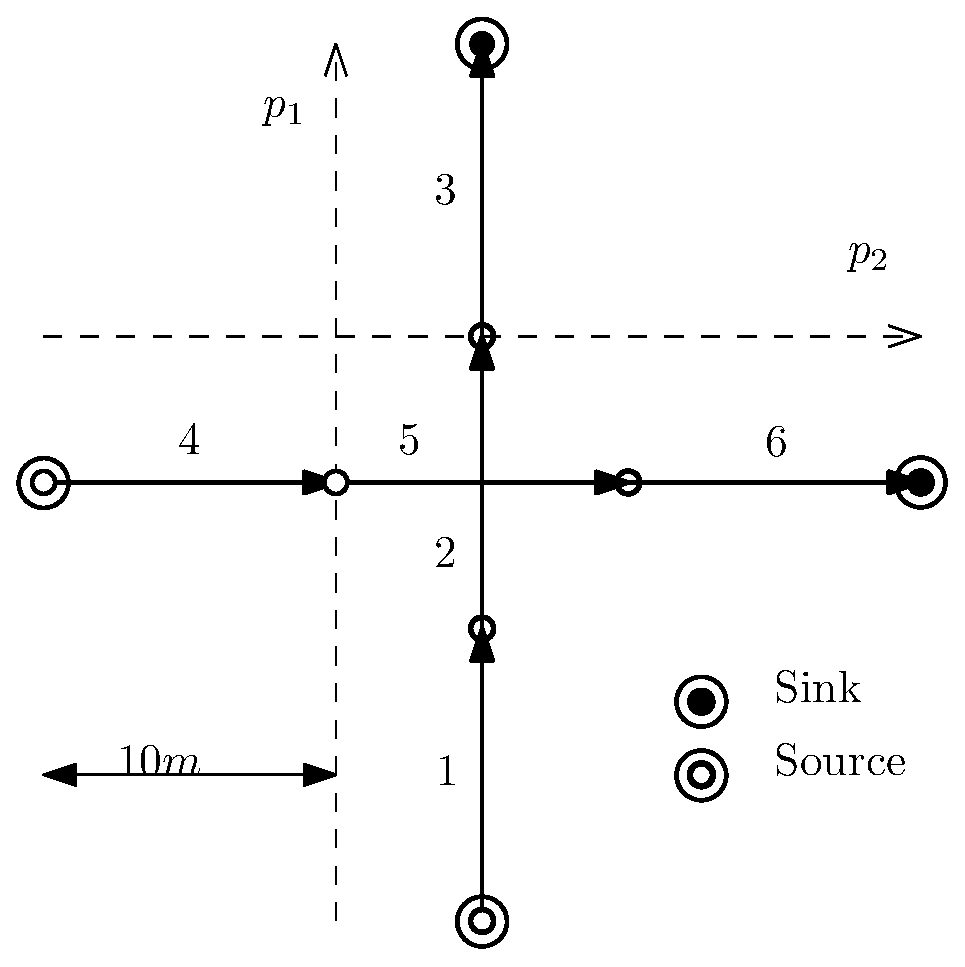
\includegraphics[width=0.9\linewidth]{intersection_topo}
	\caption{Intersection layout with two conflicting routes.}
	\label{fig:intersection_topo}
\end{figure}

The different approaches to intersection control were evaluated on a simulation of a simple intersection, comprised of two 30m lanes which cross in the middle as shown in Figure \ref{fig:intersection_topo}. There are two entrances to the map, one at the start of each lane. By varying the arrival rate $\lambda$ and the update frequency $f$, six scenarios were created with the parameters shown in Table \ref{tab:params}.
\begin{table}
	\begin{tabular}{|c|c|c|c|}
		\hline
		& $\lambda_1$ & $\lambda_2$ & $f$ \\
		\hline
		HLHT & 0.5 & 0.5 & 2 \\
		HLMT & 0.1 & 0.5 & 2 \\
		HLLT & 0.1 & 0.1 & 2 \\
		LLHT & 0.5 & 0.5 & 10 \\
		LLMT & 0.1 & 0.5 & 10 \\
		LLLT & 0.1 & 0.1 & 10 \\
		\hline
	\end{tabular}
	\label{tab:params}
	\caption{Parameters for test scenarios. All units s$^-1$. Each scenario is identified with the first two characters relating to the latency between periodic messages from the intersection controller where High Latency is 500ms and  Low Latency is 100ms and the second two relating to the arrival rate, where High Traffic has $\lambda$=10 arrivals per second on both approaches, Low Traffic has $\lambda$=2 arrivals per second on both, and Mixed Traffic has one lane with $\lambda_1$=10 and the other with $\lambda_2$=2. For example High Latency, High Traffic becomes HLHT}
\end{table}

\subsection{Trajectory Comparison with Fixed Arrival Pattern, 30 Second Run}
\label{sec:fixed_arrival_pattern}
\begin{figure}
	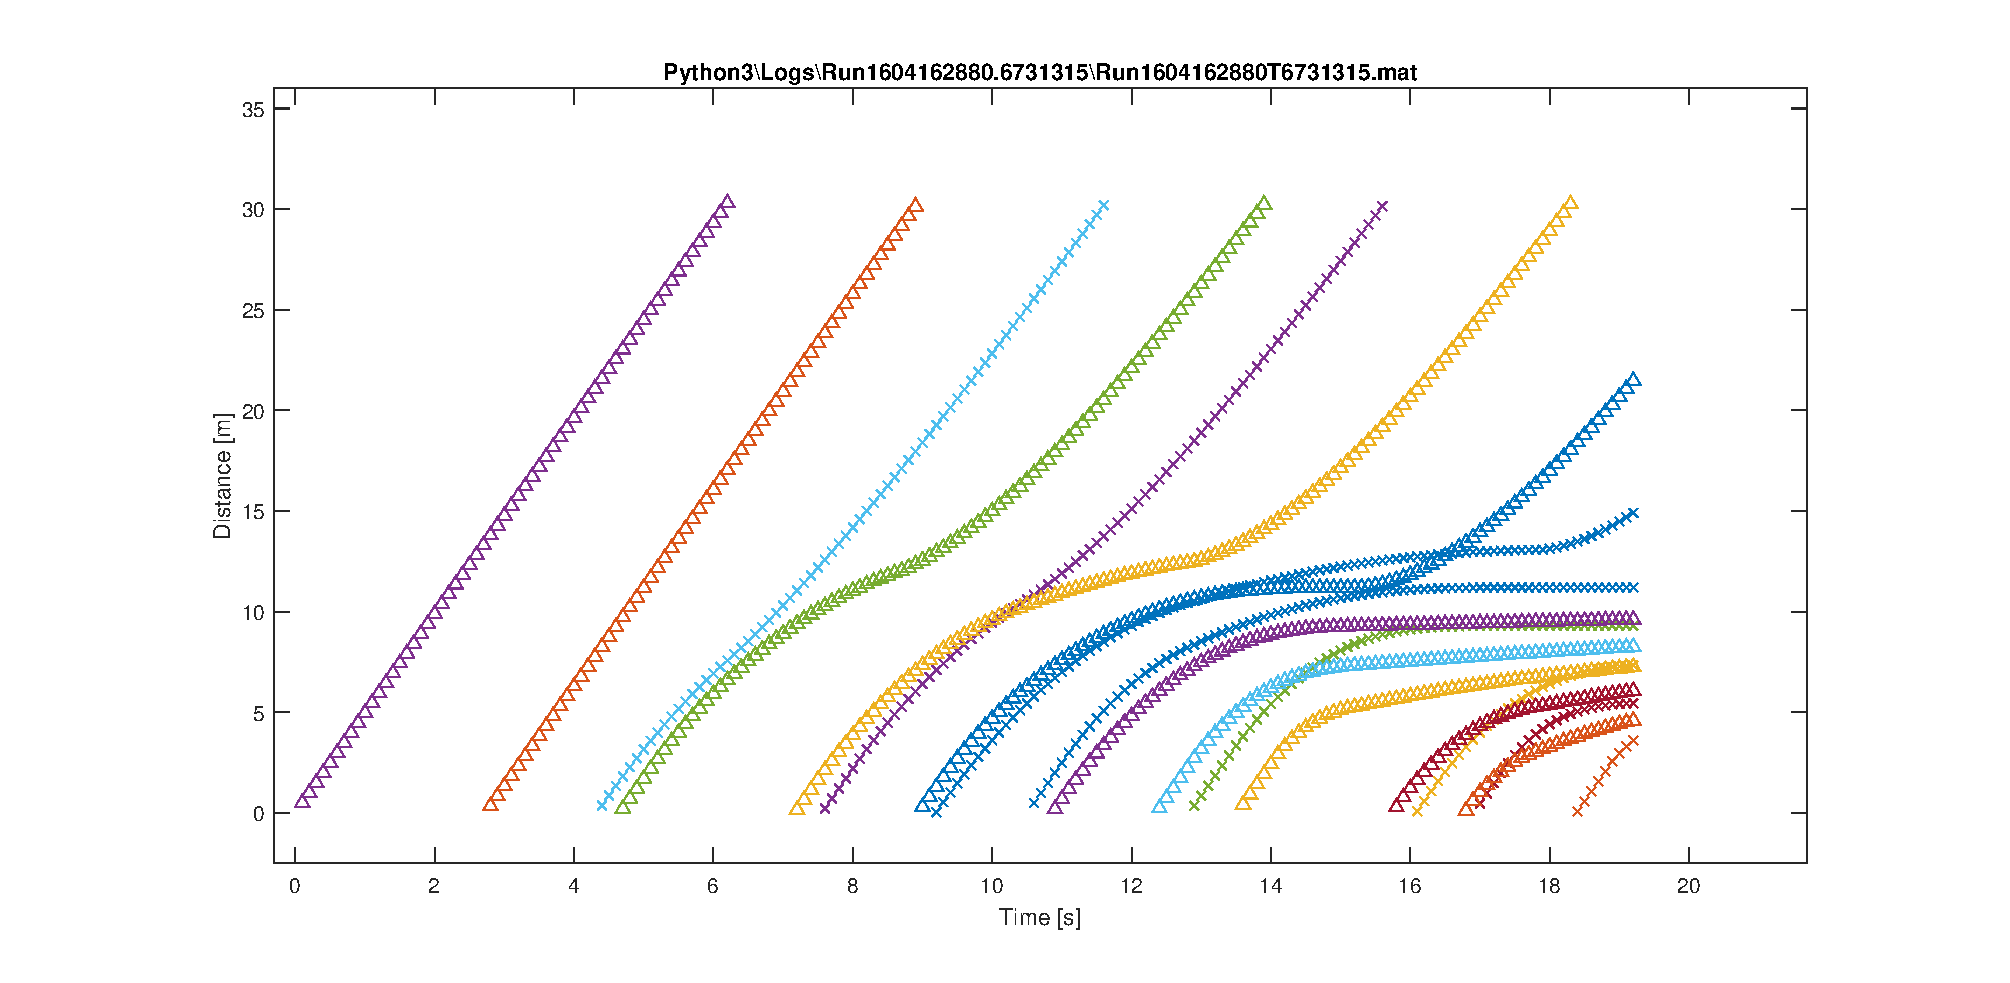
\includegraphics[width=1.0\linewidth]{SemaphoreTracesT6731315.eps}
	\caption{Position time series for the semaphore heuristic controller in scenario 1.}
	\label{fig:semaphore_st}       % Give a unique label
\end{figure}
The distance-time plot for the semaphore controller is shown in Figure \ref{fig:semaphore_st}. The distance axis is measured from the start of the submitted plan for the AGV. All plans start 15 metres from the conflict point on both lanes. AGV travelling in the x-direction are shown with 'x' markers, while those travelling in the y-direction are shown with triangle markers. The simulation did not proceed beyond 20 seconds because of a collision with a new arrival. 

\begin{figure}
	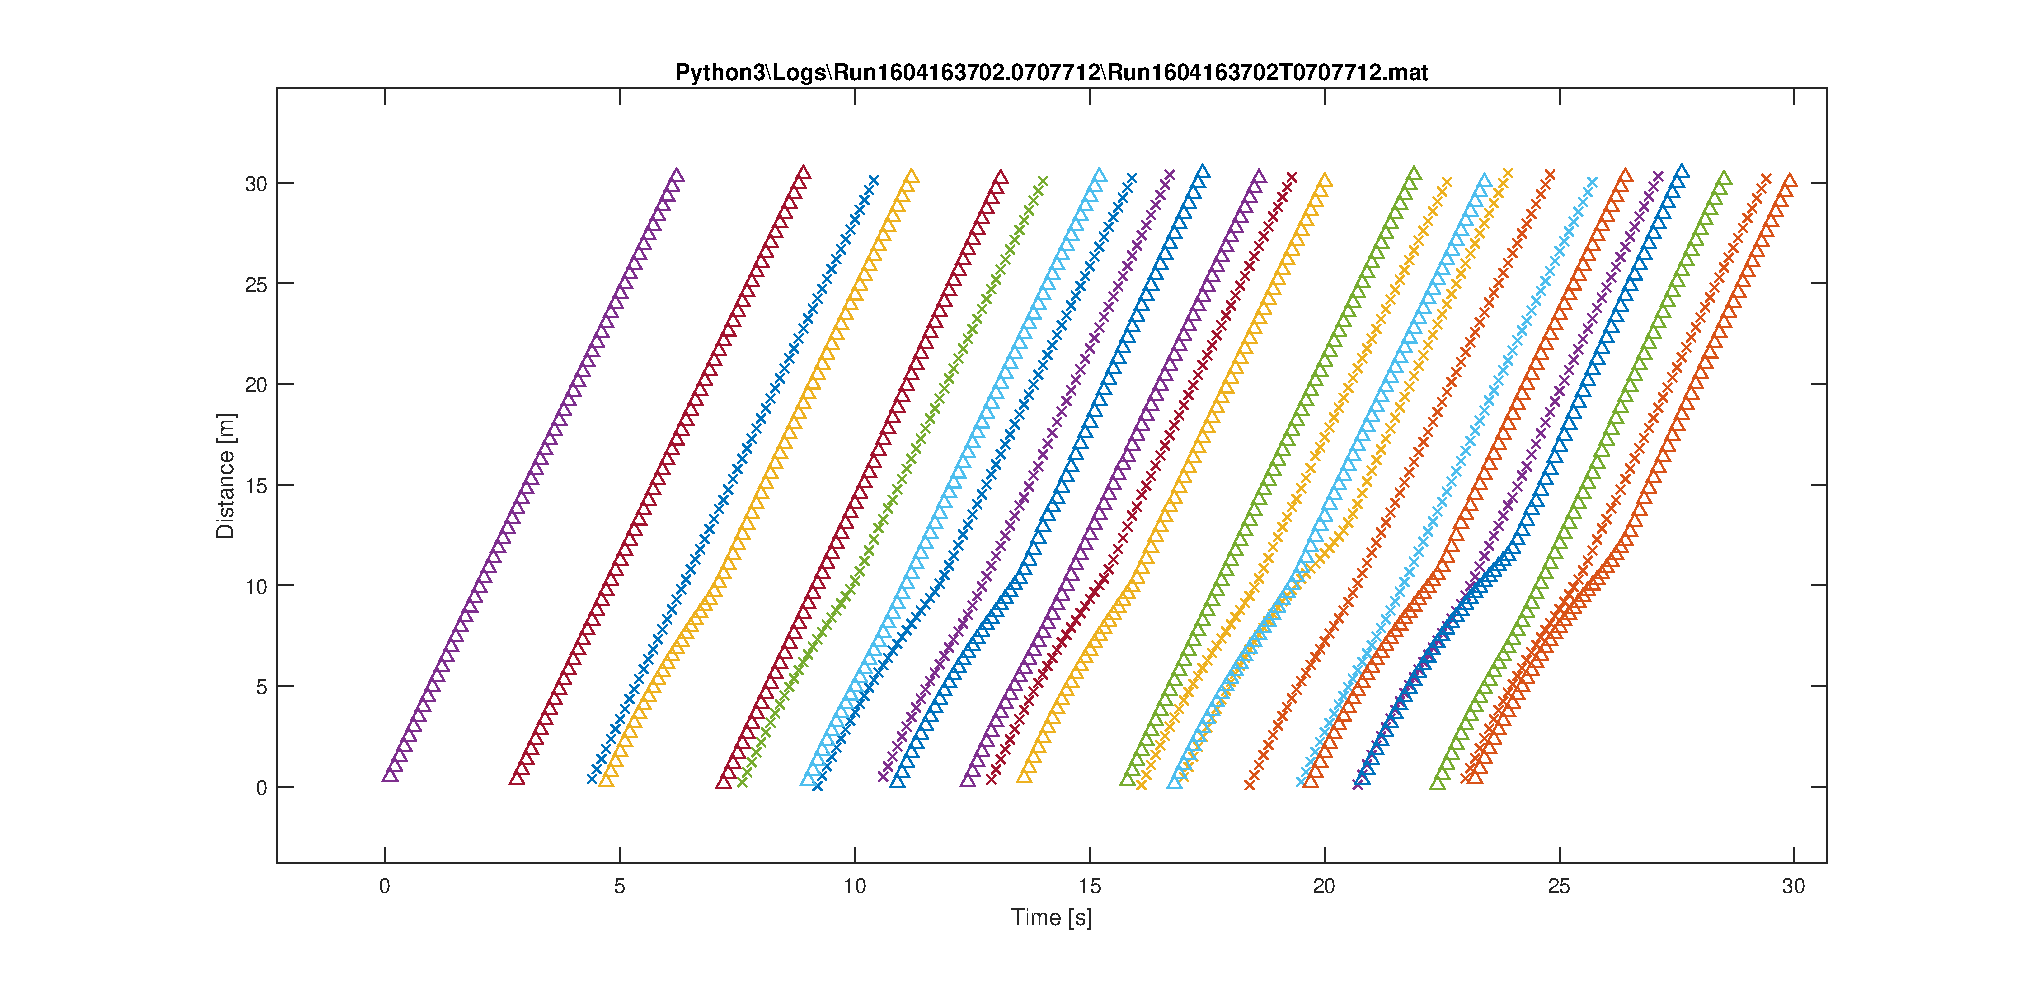
\includegraphics[width=1.0\linewidth]{OptimalFIFOTracesT707712-fixed.eps}
	\caption{The position time series for the FIFO Optimal Controller in scenario 1.}
	\label{fig:optimal_fifo_st}       % Give a unique label
\end{figure}
The distance-time plot for the FIFO Optinal Controller is shown in Figure \ref{fig:optimal_fifo_st}. It was able to proceed for the full 30 seconds without any collision as the approach lane did not fill up. This only shows that the throughput of the FIFO optimal control is higher than semaphore method, and is sufficient to meet the demand of $\lambda=0.5$ on each lane, without a queue forming.   

In these two runs the arrival sources were not linked to the occupancy af the approach lane, so if the approach lane fills up, and average speed drops, so the new arrivals can appear right on top of vehicle at the back of the queue, leading to a collision which the interseciton controller is unable to prevent.  This is not a realistic crash situation because in a real site approaching vehicles will detect the back of queue with their front safety sensor and stop in time. 

In Figure \ref{fig:optimal_fifo_st} it can be seen that 24 vehicles pass through the intersection in 30 seconds. This is very close to the upper limit of one vehicle per second determined by on the arrival rate. 

\subsection{Trajectory Comparison with Dynmaic Arrival Pattern, 30 Departures Run}
\label{sec:mutex_arrival_pattern}
To understand more about the performance of the controllers the arrival pattern was linked to the appraoch lane occpancy. Rather than deal with the complexity of speed reductions due to safety sensors, the model was based on a roadmap reservation system which are widely usedin centralized or decentralized form. The capacity of the approach lane (10 metres long) was set to 1 AGV. If the static arrival pattern suggested an arrival while the lane was full, it entered an arrival queue. At the next simulation time step where the approach lane had capacity, if there was any vehicles in the queue, the first would be introduced to the simulation at the start of the approach lane with zero speed (as opposed to the random arrivals, which enter the lane at full speed).  
\begin{figure}
	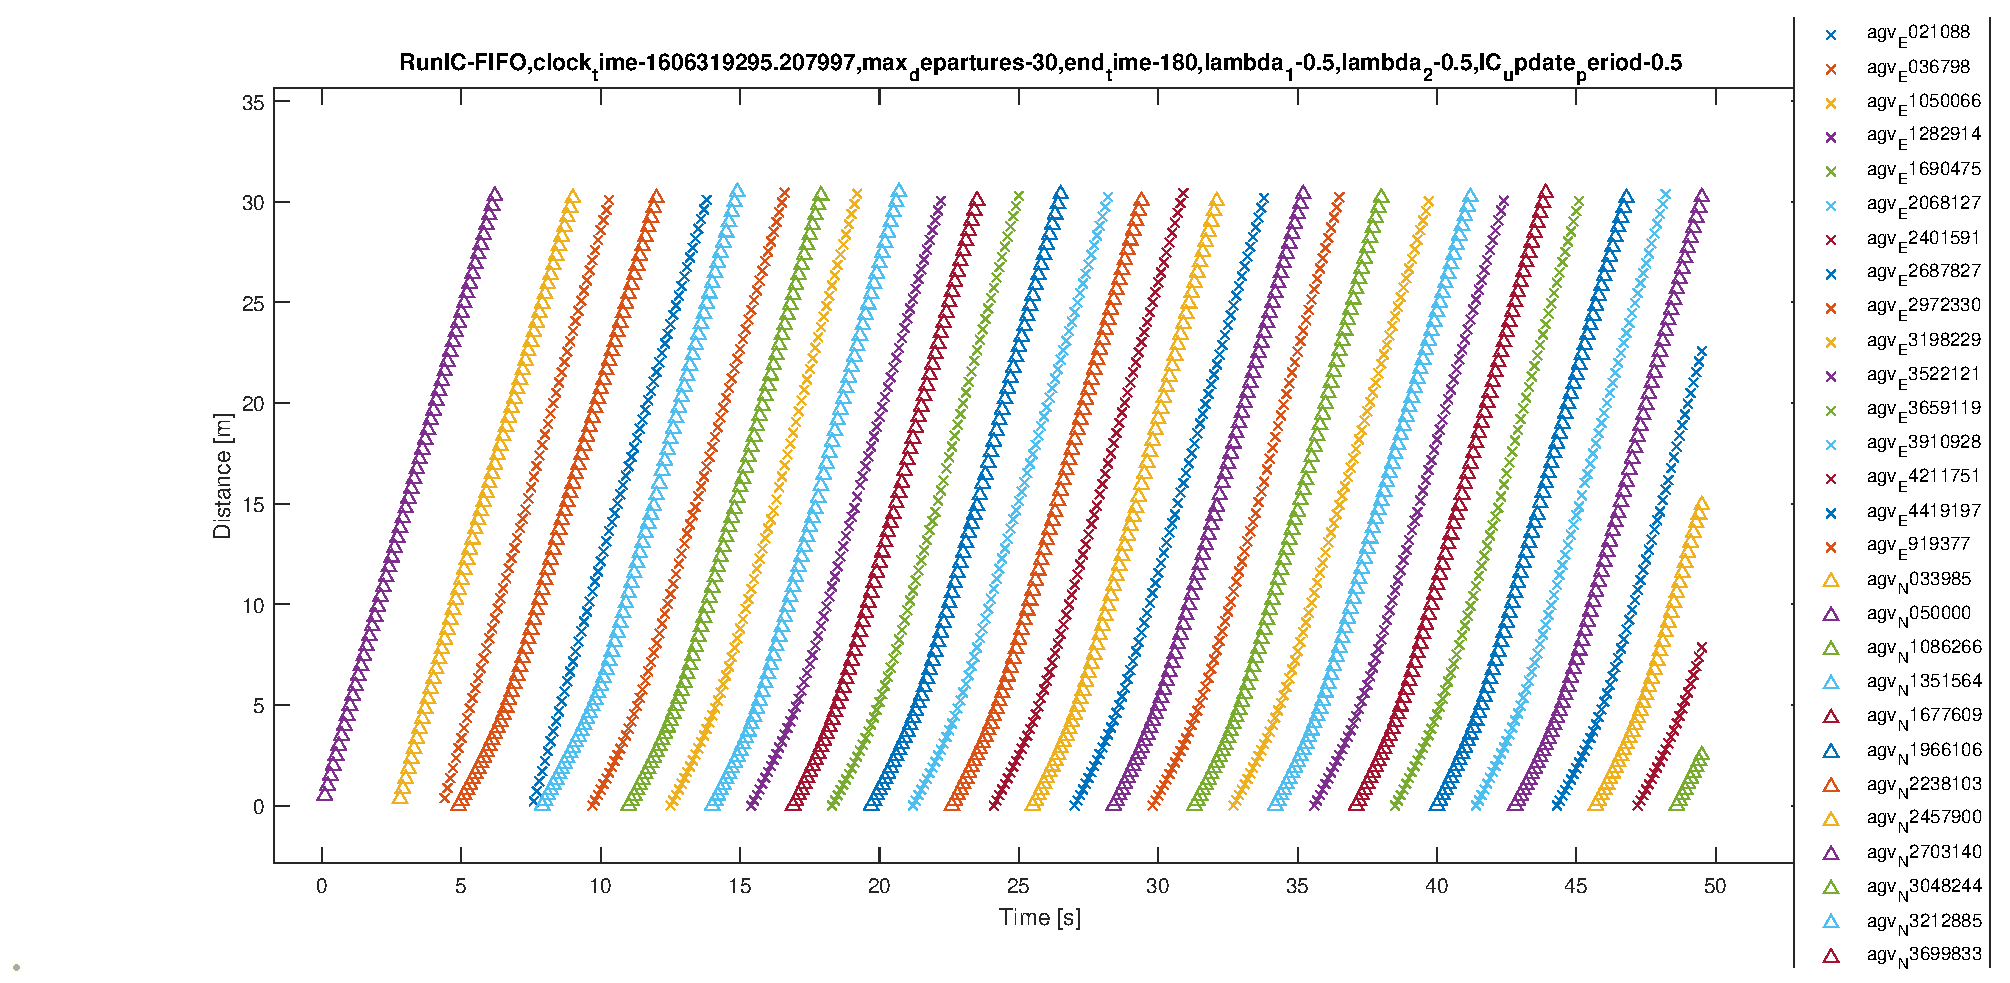
\includegraphics[width=1.0\linewidth]{distance-time-FIFO-HighLatency-HighTraffic.eps}
	\caption{The position time series for the FIFO Optimal Controller in the High Traffic High Latency Scenario}
	\label{fig:optimal_fifo_st_HL_HT}       % Give a unique label
\end{figure}
\begin{figure}
	\includegraphics[width=1.0\linewidth]{Sempahore-716956HighTraffic-HighLatency.eps}
	\caption{The position time series for the Semaphore Controller in the High Traffic High Latency Scenario.}
	\label{fig:semaphore_st_HL_HT}       % Give a unique label
\end{figure}

With arrival lane capacity of one AGV, 30 AGVs were able to cross the intersection in 82.3 seconds with the semaphore control. With FIFO optimal control this was reduced to 49.6 seconds. This is a reduction of 39.7\%, entirely due to centralized speed choice, as both used FIFO ordering. The centralized optimal FIFO controller is able to predict when the conflict will become unoccupied, so following vehicles don't need to slow down as much as with Semaphore control. 

The free flow time to cross 30 metres at maximum speed of 5 metres per second is six seconds. The mean travel time across the Semaphore controlled intersection was 309.1, indicating a delay of 309.1/30 - 6 = 4.30 seconds. The delay due to the FIFO Controlled intersection was 195.1/30 - 6 = 0.50s. This dramatic reduction might be expected given the objective for the FIFO optimal method was to minimise total travel time.   

\subsection{Energy Consumption}
The use of an approach speeds minimising total travel time increases the energy consumption per vehicle as shown in Table \ref{tab:energy_res}. The extra information about the departure time of leading vehicles should lead to reduced energy expense slowing down. As total energy usage (and therefore usage per vehicle) actually increase, and air resistance was not considered,  it suggests the higher average speeds reduce the efficiency of the motor.

\begin{table}
	\begin{tabular}{|c|c|c|}
		\hline
		& Semaphore & FIFO Optimal \\
		\hline
		Total Electrical Energy (MJ) & 542.310& 641.170\\
		Total Mechanical Energy (MJ) & 61.549& 68.448\\
		Completion Time (s) & 82.3 & 49.6\\
		Total Travel Time (s) & 309.1 & 195.1 \\
		\hline
	\end{tabular}
	\label{tab:energy_res}
	\caption{Energy and Completion Time Results }
\end{table}

\begin{figure}
	\includegraphics[width=1.0\linewidth]{agv_e_021088_power_-FIFO-HighLatency-HighTraffic.eps}
	\caption{The power dissipated over time for one AGV under FIFO control.}
	\label{fig:021088power}       % Give a unique label
\end{figure}
\begin{figure}
	\includegraphics[width=0.45\linewidth]{agv_e_021088_power_-FIFO-HighLatency-HighTraffic_zoom_out.eps}
	\caption{Spurious data points of the power dissipated over time for one AGV under FIFO control.}
	\label{fig:021088power_spurious}       % Give a unique label
\end{figure}

\begin{figure}
	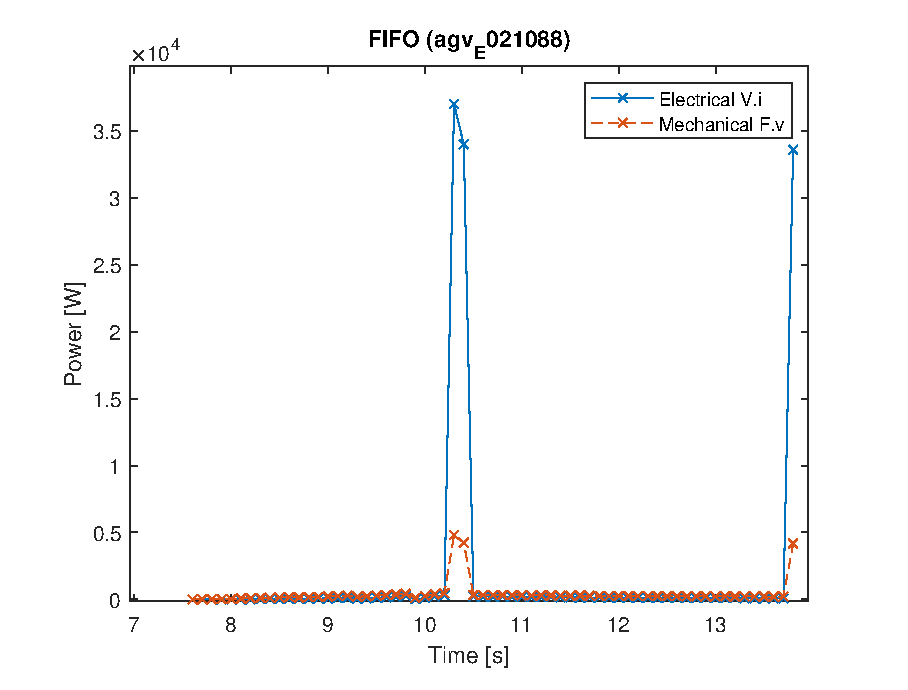
\includegraphics[width=1.0\linewidth]{agv_e_021088_power_-FIFO-HighLatency-HighTraffic-recalc.eps}
	\caption{The electric power was recalculated from the logged value of armature current $i^2$R with a resistance of R=0.001$\omega$. The mechanical power weas recaluclated using the abs(motive\_force*velocity).}
	\label{fig:recalc_021088power}       % Give a unique label
\end{figure}

\begin{figure}
	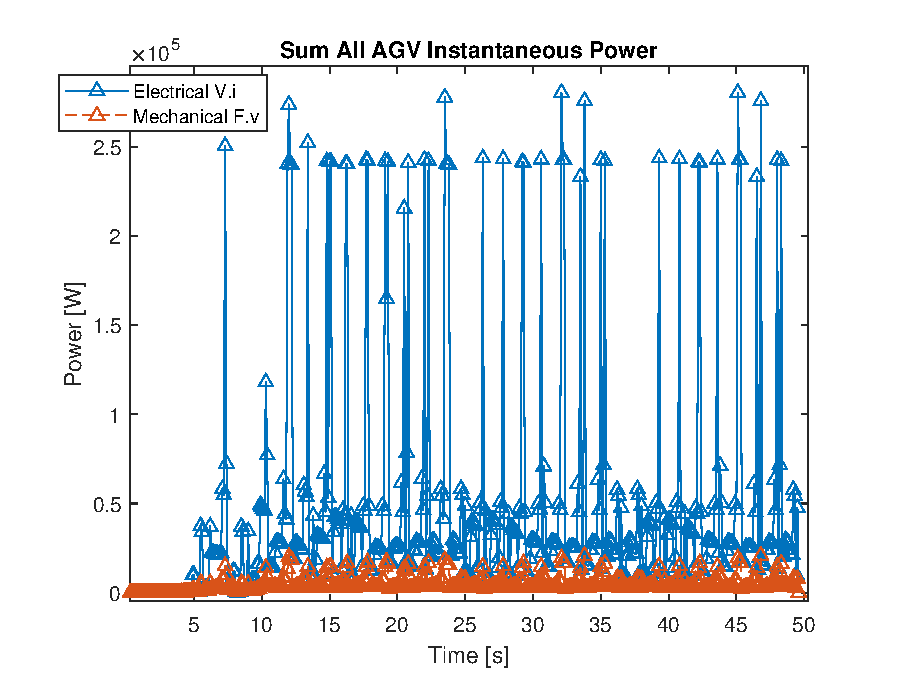
\includegraphics[width=1.0\linewidth]{fifo_power_recalc_sum_all_agv.eps}
	\caption{The power dissipated over time for all AGVs in total under FIFO control.}
	\label{fig:fifo_power_sum}       % Give a unique label
\end{figure}
\begin{figure}
	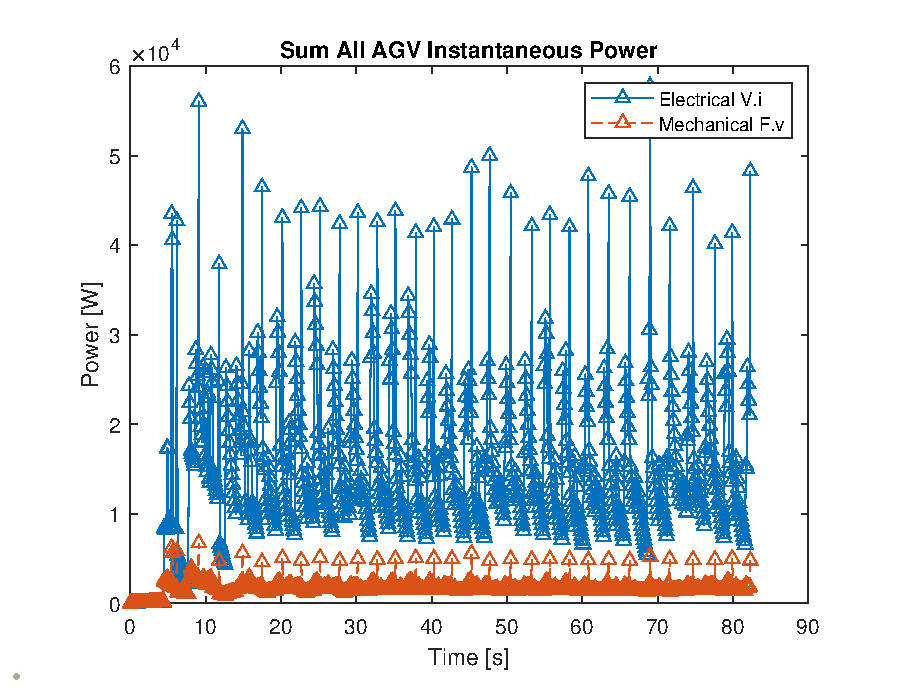
\includegraphics[width=1.0\linewidth]{semaphore_power_recalc_sum_all_agv.eps}
	\caption{The power dissipated over time for all AGVs in total under Semaphore control.}
	\label{fig:semaphore_power_sum}       % Give a unique label
\end{figure}

%\section{Literature Review} 
Studies on the theoretical capacity of signalized intersections and roundabouts with an equivalent footprint indicate that in most cases, if there are few approach lanes small roundabouts will tend to have higher capacity. If there are many approach lanes signals tend to be more effective, unless the traffic on different approaches is extremely unequal \cite{Jian-an2001}. 

A systematic procedure computing the conflict points in an intersection is given in \cite{Lu2013}. Roundabouts tend to have a large number of merging and diverging conflicts, but fewer or none of the crossing and head-on conflicts which lead to the most serious collisions due to high relative speeds.

Intersection control often addresses crossing conflicts by separating vehicles in time, while they all take the shortest path straight through the intersection in the same way as if it was signal controlled. There are a wide range of optimal and heuristic approaches to solve for the speed profile, both decentralized and centralized, a good review is given in \cite{Rios-Torres2017}. Many studies have looked at how to incorporate a proportion of human controlled vehicles which are not able to communicate their intention. One way of doing this is using traffic signals which only apply to human drivers \cite{Zhao2019}. The downside is that the nature of the intersection must remain similar to a traffic-light controlled one if non-communicating participants are going to be controlled by lights.

Recently a number of studies have extended intersection coordination of Connected and Autonomous Vehicles (CAVs) to the resolve the type of merging of diverging conflicts which occur and roundabouts. These are reviewed in \cite{Rios-Torres2017}. A centralized solution with an intersection manager minimizing delay and energy consumption is described in \cite{Zhao2018}. This shows that a high proportion of vehicles need to be communicating for significant benefits to be realized. 

A decentralized approach based on intent communication by way of virtual vehicles, can also be applied to roundabouts. In \cite{Debada2016}, reactive heuristics are shown to lead to poor performance compared to a model predictive control approach. The virtual vehicle concept allows common lane based heuristics such as car following to be extended to resolve conflicts in  \cite{Debada2018}. Another work investigating virtual lanes is \cite{Xu2018}. Here a conflict graph is used to assign approaching vehicles to appropriate virtual lanes and a distributed controller is presented to stabilize the platoon.

Another approach presented in \cite{Liu2018} is a decentralized solution to the global problem of minimizing the delay. Proofs of completeness and optimality of the aggregate problem are given, making this technique very impressive. It is not shown to be applicable to roundabouts in any of the numerical examples, although the incorporation of optimal trajectory planning by the low level controller to execute merging makes it a good example of the combination of path planning and intersection management. Collision constraints are based on a conflict zone rather than conflict points as in \cite{Levin2017}. The location of the conflict points is fixed by the fixed paths between the entry and exit lanes of the junction. The space inefficiency of the zone representation for multiple lanes is addressed by using multiple zones, one for each pair of lanes. The use of simultaneous path optimization might be expected to increase computational complexity and thereby reduce the number of vehicles with can be routed, however an attached video showing many vehicles interacting for about 10 minutes seems to refute this. It seem the ordering problem is resolved in a decentralized way based on game theory and the game `Chicken.' Using game theory to resolve the ordering problem may give this approach an edge over the mixed integer optimization used in \cite{Levin2017}, in terms of how many vehicles they can control before running into execution time limits. It is a little surprising that the game would always produce the optimal ordering given the motion model used by each AGV. The consensus mechanism will be important here. Questions remain about the possibility of AGVs disagreeing about the order they calculate from the communicated position and speed data. 

A similar method which solves the ordering ordering problem sequentially, followed by individual optimization of the approach speed along fixed paths is described in \cite{DeCampos2017}. This method claims only local (per-vehicle) optimality for the speed choice sub problem, and makes it clear the crossing order at convergence will be suboptimal, and depends strongly on the decision order. The sub problem is posed as a Linear Quadratic Regulator, commonly seen in optimal control problems. In general terms, those early in the decision order will deviate from the plans less. This is more of a problem when vehicles are not uniform, as to reduce energy consumption a late arriving lorry should deviate as little as possible. A heuristic is given for the decision order based on the time to conflict arrival.

The use of optimal control in \cite{DeCampos2017} is shared with many earlier works regarding coordination of Unmanned Arial Vehicles, many of which relax the assumption of static paths. In this way \cite{Schouwenaars2004} addressed the full multi-vehicle motion planning problem for small numbers of aircraft with simple dynamics. The craft were assumed to be differentially flat: that is, able to actuate in any of the workspace degrees of freedom independently, like a quadrotor. They were represented using bounding rectangles, leading to a slightly conservative mixed integer problem. The integer variables are used to choose which constraints are active. This might seem excessive when representing static obstacles, however when the constraints arise from other moving vehicles, the integer variables are a natural way to represent the passing-order problem. The scaling to larger numbers of vehicles is a particular challenge, due to the combinatorial explosion of possibilities.

An alternative approach to the coordination of differentially flat aircraft which uses a sequential solution of per-vehicle receding horizon sub problems to approximate the global solution is given in \cite{Keviczky2008}. An earlier theoretical treatment based on iterative bargaining with soft collision constraints is given by \cite{Inalhan2002}. The parameters are real numbers, and the constraints linear while the cost is quadratic. It may converge to an infeasible solution given a particular minimum safety distance even from a valid set of starting positions and speeds, and the suggested solution is to reduce the threshold until it becomes feasible.  

More recently, solutions based on Distributed Model Predictive (DMPC) control have been developed. In \cite{Dai2017}, per-vehicle optimizations runs simultaneously to reduce execution time. This ensures recursive feasibility and closed loop stability. Another DMPC approach is given by \cite{Luis2018}. This scales up to 25 vehicles in real time. the quadrotors concerned are all identical and differentially flat. For an under-actuated system like an AGV, some of the simplifications may no longer be possible. 

%\section{Introduction}

Reservation-based intersection management for preventing collisions between autonomous vehicles at intersections by V2V communication has been the topic of numerous studies considering road traffic. A good review is \cite{Chen2016}, another review focusing on optimization methods \cite{Malikopoulos2018}. Some early studies utilized a First-Come-First-Served (FCFS) policy which was shown to outperform signal control in some situations \cite{Dresner2008}. Problematic cases where performance could be worse than signal control were identified by \cite{Levin2016}. To capture the potential capacity improvements other works have used convex optimization \cite{Dai2017}.
The problem can also be posed as a mixed-integer optimization considering both the approach speed the arrival order as in \cite{Levin2017}.  
In \cite{Digani2019}, Digani et al present a per-intersection controller which calculates segment speeds for all approaching vehicles to minimize the total crossing time. They show that the reduction in crossing delay is far more than the increase in computation time for a realistic six way intersection, compared to a state-of-the-art decentralized approach. Like many existing studies of AGV co-ordination it is assumed that only one AGV at a time may be present on each path segment.
%
%    
%    
%\section{Literature Review}
%...
  

\subsection{Dynamic Simulation}
In order to comment on safety performance the simulated dynamics of the AGV a custom simulation was deveoped in Python. There is a great deal of software already available for simulating vehicle interactions. We reviewed those discussed below, but found it was more approporiate to further develop the simulation used for our earlier work to answer research questions related to the operation of robotic intralogistics vehicles \cite{Lambert2020a}.

These additional dynamic effects mean the timing specification sent by the intersection controller will always be missed by a small amount as it would be if the controller was communicating with embodied robots acting in a real logistics environment. In order to comment on the total energy consumption, it would be useful to model second order dynamics, allowing the dissipated power to be approximated by the acceleration. Acceleration is a good proxy for motor power in a low speed system like logistics, where there is little air resistance but lots of stopping and starting. In order to investigate the effect of communication latency the simulation time-step should be smaller than the hypothetical communication latency for client/server control over a limited bandwidth network. Lateral tracking behaviour need not be considered if we assume all AGV are able to traverse the given path with negligible lateral error. This is not too unrealistic if the paths account for dynamic limitations limitations of the vehicles which will traverse them such as radial polynomials \cite{Digani2014obs} or clothoid transitions \cite{lambertoptimalobstacles}.

With these requirements in mind, a number of off-the-shelf traffic simulation software packages were investigated. To give a brief overview we considered traditional closed source modelling software such as DRACULA \cite{Liu2005}, MATSim \cite{AndreasHorni2016}, PTV VISSIM \cite{Kara2014} and Aimsun \cite{lenorzer2015modelling}. These are powerful tools with a focus on recreating interesting microscopic traffic behaviour arising from human driven vehicles. For example DRACULA operates on a detailed road network combined with trip matrix indicating travel demand. Vehicles enter the network according to a distribution which corresponds to the trip matrix. Individual vehicles are tracked until they reach their destination, as if they parked off the road. Average speeds are calculated based on completed trips making it possible to comment on the expected delay for a journey which began at a certain time. Different junction types with and without traffic lights are handled with custom logic and are inherently conflict-free. Longitudinal behaviour is based on the intelligent driver model of human car following which is more realistic than the earlier Gipps model, but still cannot guarantees that a safe distance will be maintained within the dynamic limitations of the vehicles, which is required to guarantee collision avoidance. SUMO \cite{Busquets2016}, is an open source traffic simulator also intended as a model of human operated vehicles. It is highly configurable, and with enough modification it would be possible to modify both the  individual vehicle logitudinal control and the intersection control to reflect the two -layer control architecture proposed by \cite{Digani2015} but the only components then reused would be the vehicle dynamcs, the position trackjing and the vizualization. The tool for generating large pattern based roadmaps based on grids or webs could be used standalone, according to the open `.net' format, based on `.xml'

Another option considered was using an existing robot dynamic simulator. Stage \cite{Vaughan2008} is designed for large numbers of robots, but is unsuitable as it relies on a first order dynamics. Another option was Gazebo \cite{Rivera2019} which has been used in similar works such as \cite{Walenta2017} and \cite{Yan2017}, where ROS (Robot Operating System) libraries were used to implement the control algorithms, so the same binaries could equally be linked to a full Gazebo simulation or a collection of physical test robots. This is a great option but would force us to implement robust lateral control and other systems needed for a real AGV which are incidental to our contribution. %In \cite{Digani2019}, leveraged an industrial partner to fill this gap. 
ROS1 also has some issues with multiple vehicles which require another system to work around, for example another library Fawkes in one notable competition \cite{Niemueller2017}. An better option would be the new ROS2 library which does away with the single master architecture and TCP messaging protocol \cite{Eros2019} but is more sparsely documented and under active development at the time of writing, so we leave it for further work. 

%Initial experiments reported in \cite{Lambert2020a} and \cite{Lambert2020b}, made use of a bespoke Python simulation. We continued to develop this custom simulation to add the required functionality, instead of heavily modifying an existing microsimulation package or adding multiple vehicles to a dynamic simulator like Gazebo. The Python files for our simulation, and all the tested controllers are available in GitHub \cite{Lambert2020}.   

\subsection{Roadmap-based AGV System}
In general, a demand responsive AGV system for intra-logistics or a smart factory is concerned with completing a series of material transfer tasks. Each task consists of moving one unit load from a given pick location to the specified drop location. A well known solution to motion planning in a well known environment involves simplifying the free space into a (possibly irregular) lattice of reachable states, connected by arcs if there exists a feasible transition from one state to the other, to create  roadmap which can be encoded as a graph. A sequence of intermediate positions associated with each arc is sometimes stored alongside to avoid online re-computation. Using the roadmap graph, motion plans between any two states can be generated using a shortest path algorithm, which are detailed enough to be followed by the lateral position controller on board the vehicle. 

In a centralized system the transfer tasks are assigned to available AGVs by a single scheduler which is aware of the status of every task and the position of every vehicle. The optimal assignment would minimize the makespan or total time for the completion of all tasks, but in practice this may be too time consuming, especially if new tasks are being generated all the time like in a fulfilment centre, and different heuristics such as nearest-first assignment are useful. Conflict-free route planning depends on the task assignment and can be solved for jointly along with the assignment or performed sequentially based on a fixed assignment by searching the space time extended network to guarantee collisions are avoided.

Recently a number of decentralized systems have been developed which offer advantages in the number of vehicles that can operate in one area. In \cite{Walenta2017}, a roadmap representation is still used, but the roadmap is shared between vehicles. The partially decentralized system described in \cite{Digani2014coord} combines traffic routing with per-intersection control is primarily roadmap based. In \cite{Cardarelli2017} is it improved with the possibility for an AGV to deviate from the roadmap based on its own sensors and based on a shared sensor state called the global live view. In such a decentralized system, an intersection controller cannot be assumed to know the motion plan of approaching vehicles, unless they communicate their intention as part of the protocol. To this end it is assumed a channel exists with sufficient bandwidth and a fixed latency $T$ for the messages described in Section \ref{sec:dual_waypoint}.

\subsection{AGV Motor Dynamic and Electrical Model}
For the dynamics, every AGV was assumed to have the same mass $M=100$kg whether loaded or unloaded, reflecting a negligible cargo mass, for example spare parts for mobile phone repair. An AGV may be propelled by brushless DC motors, which provide high torque and efficiency. Even so, a major source of power loss is internal resistance of the windings and magnetic losses in the core.  %This is captured in the equivalent circuit with one lumped resistor $R$ shown in Figure \ref{fig:dc_motor}. Suitable parameters for the equivalent circuit are shown in Table \ref{tab:params} and were found in a test of an electric bicycle \cite{Racewicz2018}.
The field strength of the magnets, the number of poles and the number turns of the armature coils can be captured in the motor constant $k_T $ relating torque $\tau$ [Nm] to armature current.

\begin{equation}
\tau = k_T I_a
\label{eq:torque_constant}
\end{equation} 

Similarly, the rotational speed $\omega$ [rpm] is related to the back emf $\epsilon$ [V] by Equation \ref{eq:emf_constant}.

\begin{equation}
\omega = {k_e}\epsilon_D 
\label{eq:emf_constant}
\end{equation}

These can be combined to give the plant model for one AGV in Equation \ref{eq:model}

\begin{equation}
\ddot{x} =\frac{ u \cdot k_T (V_{CC} - \epsilon_D) }{M R_a d_W/2}
\label{eq:model}
\end{equation}

 There are numerous loss sources in an electric motor such as winding resistance, flux leakage, eddy currents in the core and so on \cite{Sarlioglu2016}. By using real-world measured mechanical power output and electrical input, an equivalent winding resistance $R_a$ for the simple model can be found. The parameters are shown in Table \ref{tab:motor_params}.

\begin{figure}[ht]
	\centering
	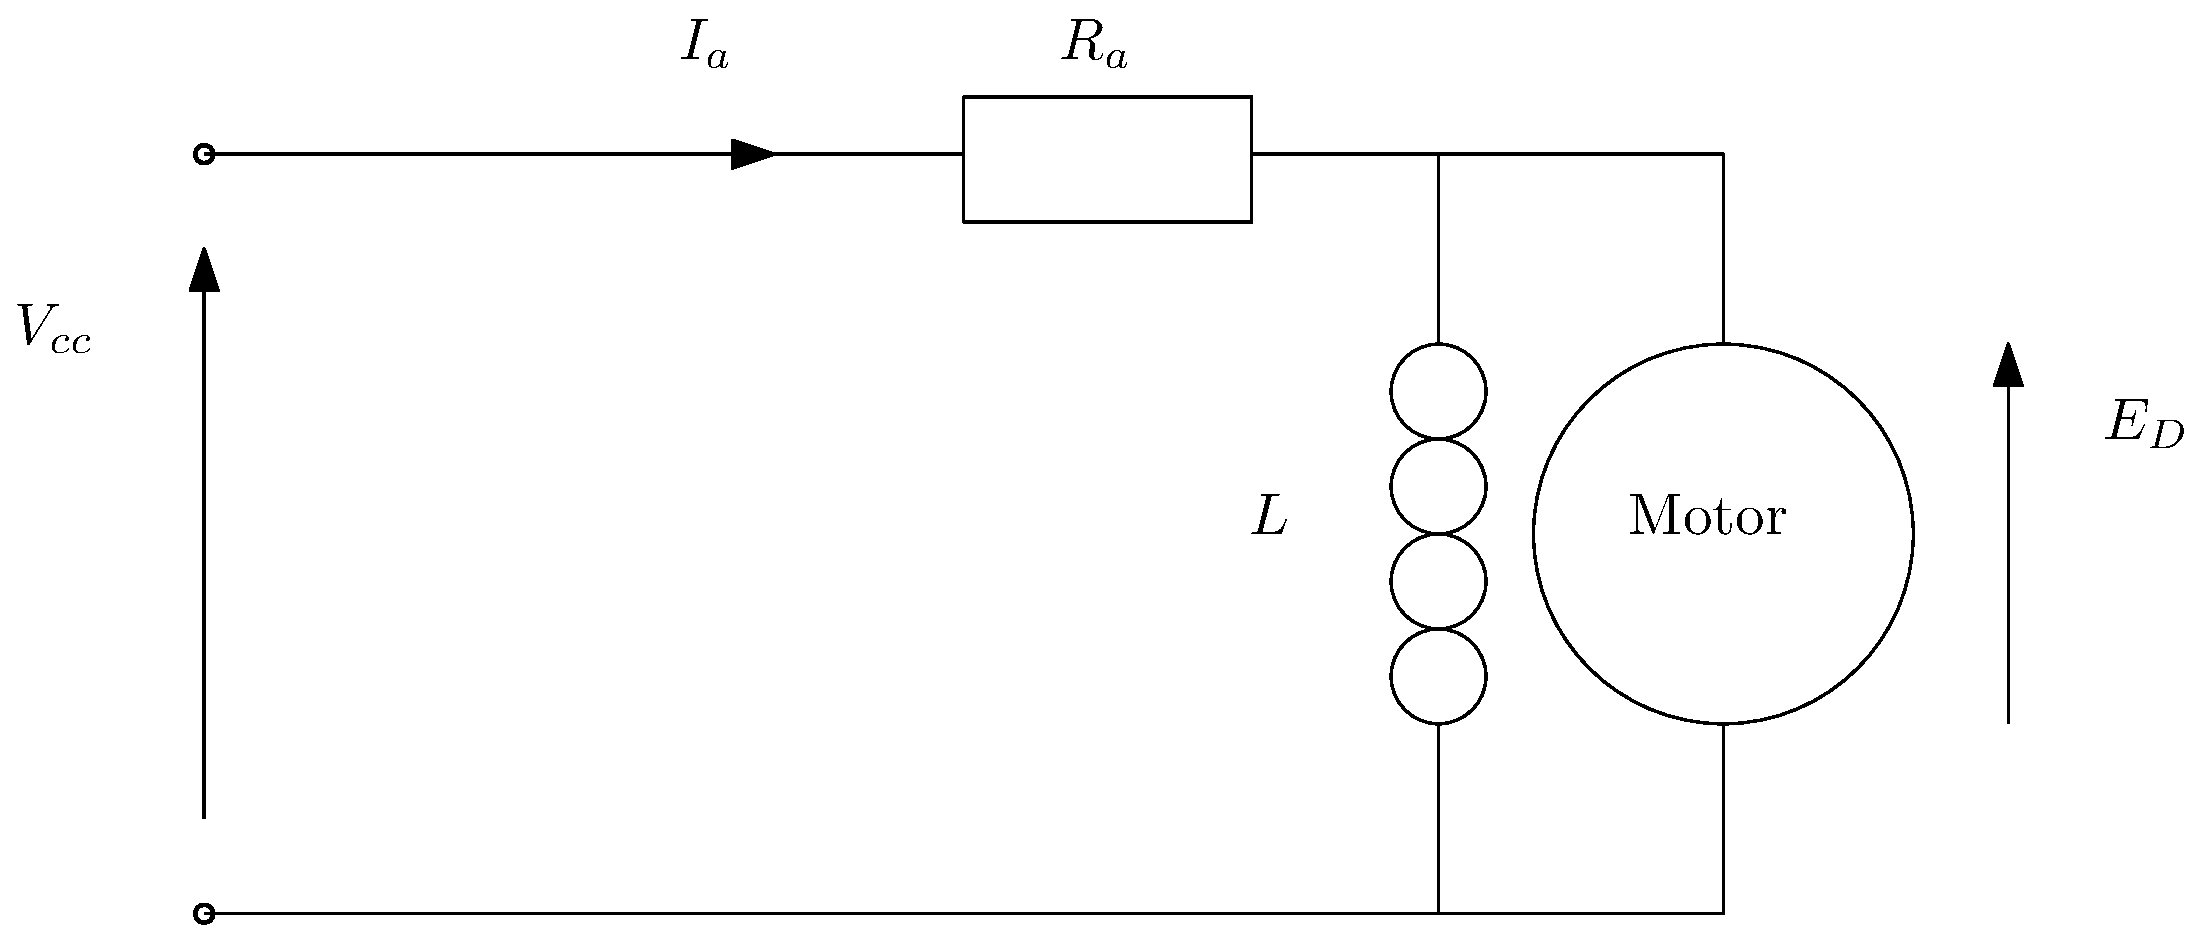
\includegraphics[width=0.9\linewidth]{dc_circuit.eps}
	\caption{Steady state equivalent circuit for a DC motor.}
	\label{fig:dc_circuit}
\end{figure}


 \begin{table}
 	\caption{Motor parameters used in simulation. Electric fork lift mass and speed \cite{Hyster2020a}. Motor and Electrical parameter from \cite{Racewicz2018}. *Computed for equivalent circuit in Equation \ref{eq:model} to match $\tau_{max}$ at $i_{max}$ }
 	\label{tab:motor_params} 
 	\centering
 	\begin{tabular}{ |c|c|c| }
 		\hline
 		$a_{max}$ & 2.5 & m/s$^2$\\
 		$v_{max}$ & 5.0& m/s \\
 		$k_v$ & 6 & rpm/V\\ 
 		$k_T$ & 1.53 & Nm/A\\ 
 		$P_{mech}@375$rpm & 3.6 & kW\\ 
 		$P_{elec}@375$rpm & 6.37 & kW \\
 		$\tau_{max}$ & 127.2 & Nm\\
 		*$R_a$ & 0.5 & Ohms\\
 		$V_{CC}$ & 72 & V\\
 		$i_{max}$ & 80 & A\\
 		$M$ & 400 & kg\\
 		$d_W$ & 0.256 & m\\
 		\hline
 	\end{tabular}
 \end{table}

As the top speed $v=5$m/s is quite low, and the vehicles stop and start frequently, air resistance which varies according to Equation \ref{eq:air_resistance} was found to be an order of magnitude smaller than the electrical losses, based on a frontal area $A=1$m$^2$ and the The drag coefficient $C$=1 for a cuboid shape was used, taken from \cite{Toolbox2004}. Air density is taken to be $\rho=1.224$kg/m$^2$.

\begin{equation}
F_a = C\rho A v^2 
\label{eq:air_resistance}
\end{equation}

A brushless DC motor for an industrial vehicle typically has a constant voltage from a battery pack \cite{Hyster2020a}. In this case we set $V_a=$72V, within the range tested in \cite{Racewicz2018}. Torque can be varied from zero to maximum by changing the slip angle between the magnetic field generated digitally by the three phase coils and the magnetic field generated by the hgh strength magnets fixed on  the rotor. The output of the vehicle's longitudinal speed controller must therefore be a duty cycle $-1.0<d<1.0$. A value of zero corresponds to zero torque, where the slip angle is zero, and a value of +/-1.0 to a slip angle of +/-90 degrees where torque is at a maximum in forward or reverse respectively.

\subsection{Dual Waypoint Interface}
\label{sec:dual_waypoint}
The dual waypoint interface is designed to be decoupled from the algorithms for scheduling and routing as far as possible. In order to support decentralized routing with adaptive paths, each approaching vehicle must send an ApproachPlan message to containing a detailed plan for how it intends to cross the intersection.  The ApproachPlan contains four parameters $d =\left[ t_A, \bm{X}( s_A ), v_A, \bm{X}(s) \right]$. The plan consists of a transmission timestamp $t_A$, a measured position $\bm{X}(s_A)$, and speed $v_A$ at the given time and a sequence of feasible positions with no timing information, the path $\bm{X}(s)$. 

Embedding the path in each request for guidance means that approaching AGV can use obstacle avoidance planning before they enter the approach lane, and still receive the correct speeds at the intersection. As a result the size and shape of the conflict zone is not fixed but depends on the current traffic situation and the approach plans received.

The conflict zone shape is calculated by discretizing $\bm{X}(s)$ into linear segments of length $L=1$m and searching for points where the minimum distance between two segments exceeds the diameter of the AGV bounding circle, and the direction of the segment is different. This ensures there is no conflict point identified where one segment joins another, which arises when two AGV are following the same path one after the other.  

The intersection controller is responsible for generating an optimal speed profile for this path $v(t)$, to create a trajectory which satisfies the collision avoidance constraints with the trajectories of all known approaching vehicles $\bm{\xi}_i(t) \forall i \in N$. 

The trajectory across the intersection $\bm{\xi}(t)$ is found from the path $\bm{X}(s)$, the start time $t_A$ and start position $\bm{X}(s_A)$ using Equation \ref{eq:integrate}.
\begin{equation}
\bm{\xi}(t)  = \bm{X}(s_A) + \int_{t_A}^{t_L} \bm{X}\left( v(t) \right)  dt
\label{eq:integrate}
\end{equation}

The speed profile is always expressed as two average speeds for two segments. The first segment $AB$ begins at the position of the AGV at transmission time $\bm{X}(s_A)$, and ends at the nearest edge of the intersection conflict zone $\bm{X}(s_B)$. The second segment $BC$ begins at $\bm{X}(s_B)$ and ends at the far edge of the intersection conflict zone $\bm{X}(s_C)$.  

To represent this level of detail, the DualWaypoint contains four parameters $d =[t_B, t_C, s_B, s_C]$. These are independent of the discretization in the ApproachPlan, and expressed in path coordinates. The flow of messages over time is shown in Figure \ref{fig:dual_wp_message_sequence.}

\begin{figure}[ht]
	\centering
	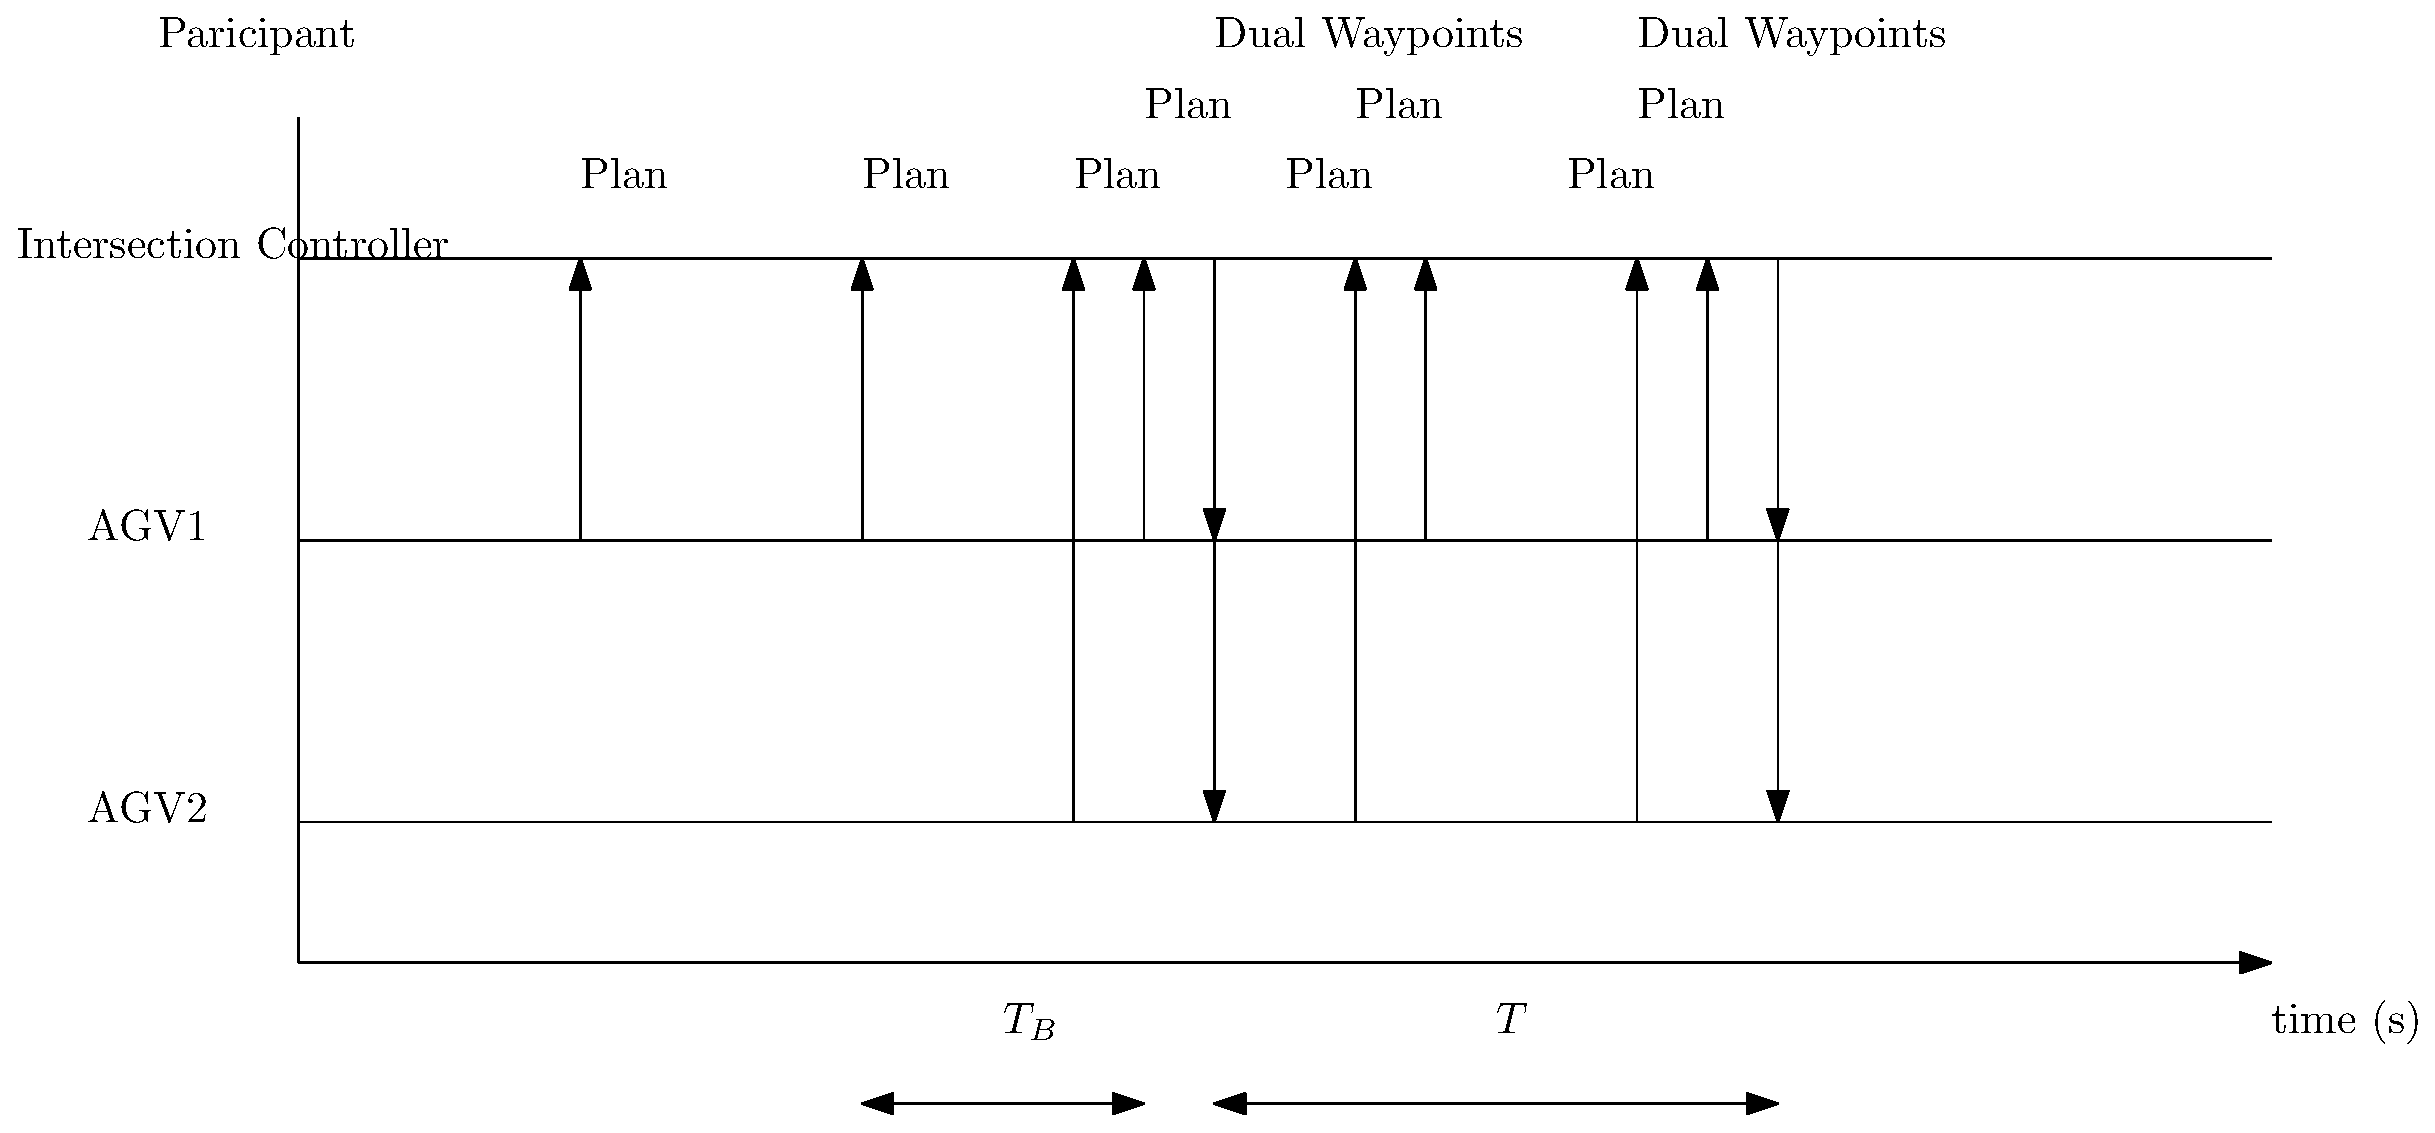
\includegraphics[width=0.9\linewidth]{dual_wp_message_sequence.eps}
	\caption{Sequence diagram for two AGVs communicating with the Intersection Controller which sends a DualWaypoint message to every known AGV every $T$ seconds, considering the latest ApproachPlans it has recieved to date. }
	\label{fig:dual_wp_message_sequence}
\end{figure}


\subsection{Longitudinal Speed Control}
Longitudinal Speed Control for each Individual AGV is based on two main behaviours. The first one determines the speed on unconflicted links. The second one is required meet the timing specification contained in the Dual Waypoint message, subject to disturbances and uncertainty in the plant using position feedback.  

Previous authors have modelled the speed on unconflicted links using car-following behaviour models. Automated traffic is assumed to follow an Adaptive Cruise Control Model with set headway, while human operated vehicles follow the Intelligent Driver Model in \cite{Baz2020}. In the AGV space it is common to simplify car-following with mutual exclusion of discretized roadmap segments  \cite{Digani2014coord} so we follow this scheme for the main results. Some results with mutual exclusion turned off are given in  in Section \ref{sec:fixed_arrival_pattern} before the main results with mutual exclusion in Section \ref{sec:mutex_arrival_pattern}. The update period $T_L=0.1$s must shorter or equal to that of the intersection controller $T$. 

The Dual Waypoint Timing Specification is met with a constant acceleration model based on the collision-free operation modes in \cite{He2020}. 
Our simulation incorporates two modes, depending on whether the vehicles position feedback $\bm{X}(\hat{s})$ at time $\hat{t}$ indicates it is approaching the conflict zone so $\hat{s}<s_B$ or already inside it so $s_B\leq s_A<s_C$. If the AGV has passed the conflict $\hat{s}>s_C$ then its speed is unconstrained from the perspective of this intersection controller. In the simulation exiting vehicles would accelerate to maximum speed, at $\alpha_{max}$.

On approach to the conflict zone, where $\hat{s}<s_B$, the approach acceleration $\alpha_{AB}$ is given by Equation \ref{eq:approach}.
\begin{equation}
\alpha_{AB} = \frac{(s_B - \hat{s}) - \hat{u}(t_B - \hat{t}) }{0.5 (t_B - \hat{t})^2}
\label{eq:approach}
\end{equation}

Within the conflict zone $s_B \leq s_A<s_C$ the acceleration $\alpha_{BC}$ is given by Equation \ref{eq:within}.
\begin{equation}
\alpha_{BC} = \frac{(s_C - \hat{s}) - \hat{u}(t_C - \hat{t}) }{0.5 (t_C - \hat{t})^2}
\label{eq:within}
\end{equation}

\section{Method}
To examine control of variable numbers of vehicles, and comment on safety effects as well as performance of experimental algorithms utilizing a dynamic simulation test environment seemed prudent to start with. The goal here is to examine edge cases which are safety critical (may lead to a collision between AGV). The different algorithms will be compared based on execution time, total travel time, total energy consumption and mean throughput delay with a given traffic pattern.

\subsection{Conflict Zone Approximation}
\label{sec:conflict_zone}
The collision avoidance constraints are simplified by merging all the conflicts on each path, to keep only the smallest $s_B$ and the largest $s_C$ for that path. The extent of the conflict zone for vehicle$i$ is given by Equation \ref{eq:distance_threshold}. The conflicted segment of each vehicle's path lies between $s_B$ the smallest value of $s$ which satisfies Equation \ref{eq:distance_threshold} and $s_C$ the largest value. The union of these conflicted segments form the total conflict zone, which is an irregular non-convex, connected compound shape. 

In some cases it may be advantageous to limit mutual exclusion by only considering path segments which have different orientations to be in conflict, even if they satisfy Equation \ref{eq:distance_threshold}. This could allow closer spacing of AGV travelling in the same direction by following according to the distance measured to leader by on-board sensors.

\begin{equation}
\label{eq:distance_threshold}
||X_i(s) - X_j(t)|| < W_v \quad \forall j \in N, \quad j>i\\
\end{equation}

\subsection{Objective}
The objective to minimize the total travel time is given by Equation \ref{eq:objective}. It is linear terms of the reciprocal speed vector $\bm{\phi} \in R^{(n \times n)}$, which has up to two elements per AGV. One for the approach if it has not yet been passed and one for the conflict so $\bm{\phi}_i = [\phi_{AB}, \phi_{BC}]$. The segment lengths for the approach and the conflict are contained in distance vector $\bm{d}$ so $\bm{d}_i =[d_{AB}, d_{BC}] $.

\begin{equation}
\label{eq:objective}
\begin{array}{c}
\min \limits_{\bm{\phi}} \bm{J}_T = \bm{d}^T\bm{\phi} \\ 
$subject to$\\
\bm{\phi} > \phi_{min} \\
\bm{\phi}^T \bm{H_{ij}} \bm{\phi} > 0 \quad \forall i, j \in [1,p] \quad $with $ j > i \\
\end{array}
\end{equation}

The condition $j > i$ in Equation \ref{eq:objective} indicates that the number of constraints varies with the number of vehicles $p$ as $\frac{p(p-1)}{2}$. This corresponds to one constraint between each pair of approaching AGVs.

\subsection{Differential Constraints}
Vehicle acceleration limits are dealt with implicitly, by the maximum speed which can be expressed as a lower bound on $\bm{\phi} < \phi_{min}$. The simulated value $\phi_{min}$=5m/s, is reachable within a certain distance $d_{min}$ from any feasible starting speed, assuming a constant limited acceleration $a_{max}$ according to $v_{max} = \sqrt{2 a_{max} d_{min}} $. Using the parameters from Table \ref{tab:params}, the acceptable distance is $d_{min}=$5m.

\subsection{Online Feedback Considerations}
In order to guarantee feasibility we need only to ensure the conflict zone length $d_{BC}$ and the approach length $d_{AB}$ are both greater than $d_min$ when vehicles receive their instructions. A vehicle proceeding toward the conflict will eventually pass the point of no return where $d_{AB} = d_{min}$. It can not be guaranteed that any instructions sent after this point can be satisfied by the on-board longitudinal control. Any vehicle past the point of no return appears in the optimization as a constant constraint on the speeds of subsequent vehicles. The constraint uses the latest reported speed and position for real-time feedback, so if a vehicle past the point of no return fails to meet its deadline, the later vehicles can be safely delayed until it leaves the conflict zone.  

\subsection{Conflict-zone Collision Avoidance Constraints} 
By definition, each intersection controller is responsible for one conflict zone, constructed as explained in Section \ref{sec:conflict_zone}. This makes it
possible to express the constraint that vehicles do not collide
in terms of time. Vehicle $i$ arrives at the first conflicted
segment $\omega_min$ and departs from the last at $\omega_{max}$ . The following three subsections set out three alternative ways
of expressing the collision avoidance constraints which have
been evaluated. The arrival time is given by Equation \ref{eq:arrive}. Considering average speeds, the departure time $\omega_{max}$ is also linear, this is given by Equation \ref{eq:depart}.

\begin{equation}
\label{eq:arrive}
\omega_i^{min} = d_{AB} \phi_{AB} = \bm{e}^T \bm{\phi}_i
\end{equation}

Where
\begin{equation}
\label{eq:e_vec}
\bm{e}^T = [d_{AB}, 0]
\end{equation}
and 
\begin{equation}
\label{eq:depart}
\omega_i^{max} = [d_{AB}, d_{BC}]\left[\begin{array}{c}
\phi_{AB}\\
\phi_{BC}
\end{array}\right] = \bm{f}^T \bm{\phi}_i
\end{equation}
Where
\begin{equation}
\label{eq:f_vec}
\bm{f}^T = \begin{cases}
    [d_{AB}, d_{BC}],& \text{if } d_{AB}> 0\\
    [0, d_{BC}],              & \text{otherwise}
\end{cases}
\end{equation}

Following \cite{Digani2019}, the time window between $\omega_{min}$ and $\omega_{max}$ may be expressed in terms of the midpoint $\alpha$ and the extent $\beta$. In this way the collision avoidance constraints in Equation \ref{eq:mod_cons} are independent of the order in which AGV $i$ and AGV $j$ arrive.

\begin{equation}
\label{eq:mod_cons}
|\alpha_i - \alpha_j|> \beta_i + \beta_j
\end{equation}

Here
\begin{equation}
\alpha_i = \omega_i^{max} + \omega_i^{min}
\end{equation}
represents the midpoint of the time vehicle $i$ occupies the conflicted segment and and
\begin{equation}
\beta_i = \omega_i^{max} - \omega_i^{min}
\end{equation}
represents the range of the time either side of the midpoint, both scaled by a factor of two.

In matrix form this can be written
\begin{equation}
\label{eq:alpha_mat}
\alpha_i = \bm{f}^T\bm{\phi}_i + \bm{e}^T\bm{\phi}_i = \bm{1}_i^T\bm{A}\bm{\phi}_i
\end{equation}
with $\bm{A}= $ diag$(\bm{f} + \bm{e})$
\begin{equation}
\label{eq:beta_mat}
\beta_i = \bm{f}^T\bm{\phi}_i - \bm{e}^T\bm{\phi}_i = \bm{1}_i^T\bm{B}\bm{\phi}_i
\end{equation}
with $\bm{B}= $ diag$(\bm{f} - \bm{e})$

\subsection{Extra Constraint Between Vehicles in the Same Lane}
Vehicles travelling in the same lane forming a moving queue are more constrained than vehicles approaching a conflict zone. AGV are assumed here to be unable to overtake safely based on local sensors. This is likely to hold even with recent AGV which are capable of significant autonomy including adaptive path planning. This is because floor space is at a premium in a logistic environment so the gaps between the shelves are unlikely to be much wider than one AGV.

Indices are increasing so vehicle (i+1) is following behind vehicle (i). The safety constraint between vehicles in the same lane $l$ to ensure they remain a safe distance $L$ apart is given by Equation \ref{eq:in-lane1}
\begin{equation}
s_{i} > s_{i+1} + L \quad \forall i \in l
\label{eq:in-lane1}
\end{equation}
This can be expressed in terms of minimum time to collision of $TTC_{min} = 2 L/(v_i + v_{i+1})$ as in Equation \ref{eq:in-lane2}.
\begin{equation}
(s_{i}-s_{i+1})/(v_i - v_{i+1})) > TTC_{min}
\label{eq:in-lane2}
\end{equation}

It is a little awkward to capture this constraint exactly using the average speed on two segments. This approximation in Equation \ref{eq:in-lane3} was tested.
\begin{equation}
(s_{i}-s_{i+1})(\phi_i - \phi_{i+1})) > TTC_{min}
\label{eq:in-lane3}
\end{equation}  
\subsection{Non-Convex Quadratic Constraints Optimal Intersection Control}
\label{sec:quad}
Equation \ref{eq:mod_cons} can be converted to standard form by squaring both sides and substituting the matrix expressions for $\alpha_i$ and $\beta_i$. This gives the matrix inequality for each pair of vehicles shown in Equation \ref{eq:lambda}.
\begin{equation}
[\bm{\phi}_i^T, \bm{\phi}_j^T] \left[\begin{array}{cc}
\bm{\Lambda}_{ij}^{ii} & \bm{\Lambda}_{ij}^{ij} \\
\bm{\Lambda}_{ij}^{ji} & \bm{\Lambda}_{ij}^{jj}
\end{array}\right] > 0
\label{eq:lambda}
\end{equation}

The four pairwise submatrices can be expressed in terms of the diagonalized distance $\bm{A}$ and $\bm{B}$ as follows:
\begin{equation}
\bm{\Lambda}_{ij}^{ii} =  (\bm{A}_i - \bm{B}_i)\bm{1}_i\bm{1}_i^T(\bm{A}_i + \bm{B}_i)
\end{equation}

\begin{equation}
\bm{\Lambda}_{ij}^{jj} =  - (\bm{A}_j + \bm{B}_j)\bm{1}_j\bm{1}_j^T(\bm{A}_j + \bm{B}_j)
\end{equation}

\begin{equation}
\bm{\Lambda}_{ij}^{ij} = \bm{\Lambda}_{ij}^{ji T}  =  - (\bm{A}_j + \bm{B}_j)\bm{1}_j\bm{1}_i^T(\bm{A}_i + \bm{B}_i)
\end{equation}

For more than two vehicles this can be arranged into a
block diagonal matrix $\bm{H}_{ij} \in R^{(n \times n)}$ which is compatible with the input parameters, but still only represents the constraints between a pair with zeros for the other elements. The full constraint matrix $\bm{H}$ is the sum of these pairwise matrices, for every pair with $j<i$. 


%The intersection controller's task is to search over feasible speed profiles for the set which minimizes the total travel time for all approaching vehicles to cross the conflict zone. It was implemented following the description in \cite{Digani2019}, the only change being to express the constraints in path coordinates, rather than using discrete path segments, so they match up with the DualWaypoint interface and a fair comparison can be made with the other approaches.








\subsection{First-Come-First-Served Optimal Linear Intersection Control}
With a fixed ordering such as First-Come-First-Served, the reciprocal speed vector $\bm{\phi}$ is arranged in arrival order. 

The constraint in Equation \ref{eq:mod_cons} only needs to be applied between adjacent vehicles and it will hold for all vehicles. This reduces the number of constraints between $n$ vehicles to $n-1$.

The timing constraint that the leader exits the conflict zone before the follower enters is 
\begin{equation}
\omega_i^{max} > \omega_{i+1}^{min}
\end{equation}

This can be expressed as 
\begin{equation}
\bm{e}_i^T\bm{\phi}_i > \bm{f}_{i+1}^T\bm{\phi}_{i+1}
\end{equation}

leading to a pairwise matrix $Q^{ij} \in R^{(n \times n)}$
\begin{equation}
\bm{Q}^{ij}\bm{\phi} = \left[ \begin{array}{cccc}
0 & \hdots &&\\
\hdots & \bm{e}_i^T & -\bm{f}_{i+1}^T & \hdots \\
&&\hdots & 0\\
\end{array} \right]
\left[ \begin{array}{c}
\vdots\\
\bm{\phi}_i \\
\bm{\phi}_{i+1} \\
\vdots\\
\end{array} \right]
\end{equation}

The pairwise $Q^{ij}$ matrices are added together to get $A_{ub}$ in Equation \ref{eq:lin_cons}, 
\begin{equation}
\label{eq:lin_cons}
A_{ub}\bm{\phi} > 0
\end{equation}

The vehicles past the point of no return with latest feedback reciprocal speeds for each incomplete segment
\begin{equation}
\bm{p}_k  = [1/v_{AB}, 1/v_{BC}]
\end{equation}
are included in Equation \ref{eq:exit_constr} 
\begin{equation}
\bm{e}^T\bm{\phi}_i >  \bm{f}^T\bm{p}_k
\label{eq:exit_constr}
\end{equation} 
here $\bm{f}$ defined in Equation \ref{eq:f_vec}.
 
  
\subsection{Semaphore Based Collision Avoidance}
The constraints can be enforced without any optimization using a common synchronization object the binary semaphore. This is also based on first come-first-served ordering and the intersection controller gives the semaphore to the closest vehicle who provides an Approach Plan. This requires special messages in the dual waypoint interface, as the intersection controller makes no attempt to predict the time the conflict will become free. It issues a full speed ahead command to the vehicle with the semaphore and a space exclusion to all other vehicles. This consists of a distance along the AGVs submitted plan which it is not allowed to pass until given further instructions. 

This type of system is expected to lead to sub optimal throughput but be fast to calculate and guarantees safe operation. Similar schemes have been described in the literature so it is included in the comparison to give an idea of the benefits of departure time modelling and approach speed synchronization. 

\section{Numerical Results}

\begin{figure}[ht]
\centering
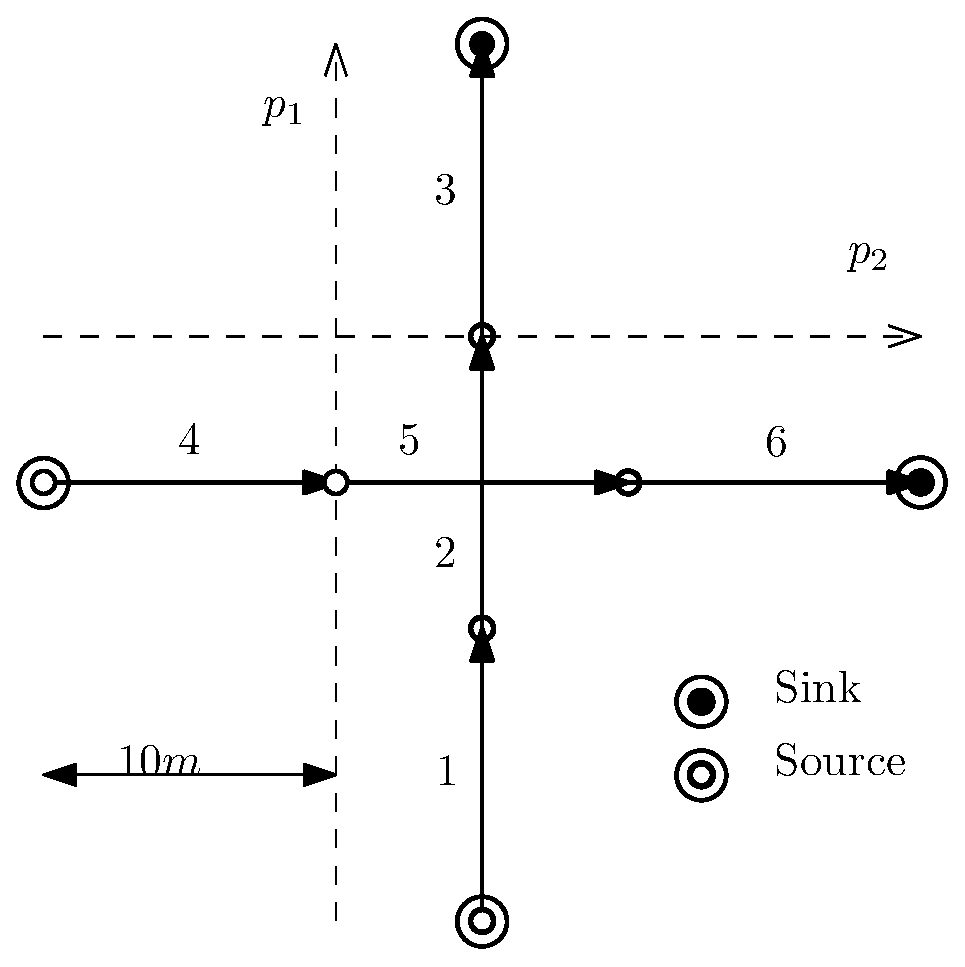
\includegraphics[width=0.9\linewidth]{intersection_topo}
\caption{Intersection layout with two conflicting routes.}
\label{fig:intersection_topo}
\end{figure}

The different approaches to intersection control were evaluated on a simulation of a simple intersection, comprised of two 30m lanes which cross in the middle as shown in Figure \ref{fig:intersection_topo}. There are two entrances to the map, one at the start of each lane. By varying the arrival rate $\lambda$ and the update frequency $f$, six scenarios were created with the parameters shown in Table \ref{tab:params}.
\begin{table}
\begin{tabular}{|c|c|c|c|}
\hline
	& $\lambda_1$ & $\lambda_2$ & $f$ \\
\hline
HLHT & 0.5 & 0.5 & 2 \\
HLMT & 0.1 & 0.5 & 2 \\
HLLT & 0.1 & 0.1 & 2 \\
LLHT & 0.5 & 0.5 & 10 \\
LLMT & 0.1 & 0.5 & 10 \\
LLLT & 0.1 & 0.1 & 10 \\
\hline
\end{tabular}
\label{tab:params}
\caption{Parameters for test scenarios. All units s$^-1$. }
\end{table}

Each scenario is identified with the first two characters relating to the latency between periodic messages from the intersection controller where High Latency is 500ms and  Low Latency is 100ms and the second two relating to the arrival rate, where High Traffic has $\lambda$=10 arrivals per second on both approaches, Low Traffic has $\lambda$=2 arrivals per second on both, and Mixed Traffic has one lane with $\lambda_1$=10 and the other with $\lambda_2$=2. For example High Latency, High Traffic becomes HLHT

\begin{table}
\begin{tabular}{|c|c|c|c|c|c|c|c|c|}
\hline
& T[s]&TTT[s]&t[s]&$\Delta$[s]&Ee[MJ]&Em[MJ]&Ex T[s]\\
\hline
FIFO & 45.7 & 181.0 & 6.033 & 0.033 & 43.906 & 30.323 & 0.0036\\
%FIFO HLMT & 70.9 & 181.5 & 6.05 & 0.05 & 52.225 & 35.083 \\
Quad & 44.8 &181.6& 6.0533 & 0.053 & 44.832 & 30.964 & 0.5252\\
%Quad HLMT & 70.9 & 181.5 & 6.05 & 0.05 & 52.225 & 35.083 \\
Sema & 83.9 & 326.4 & 10.88 & 4.88 & 159.1 & 68.140 & <0.001\\
\hline
\end{tabular}
\label{tab:results}
\caption{Intersection performance over 30 crossings with three different controllers for the HLHT scenario. }
\end{table}

The effects of the different controllers can be seen in the position time trace for 30 simulated crossings. The conflict zone is protects the intersection between the two lanes at s = 15m. Both lanes are collapsed onto one diagram, with $\times$ markers for vehicles travelling along the x axis and $\bigtriangleup$ markers for vehicles travelling along the y-axis. The controller is successful provided only one type of marker is present in the conflict zone at one time. All controller are safe, so the main comparison is how much the vehicles must slow down, shown by the gradient of the lines.  
\begin{figure}
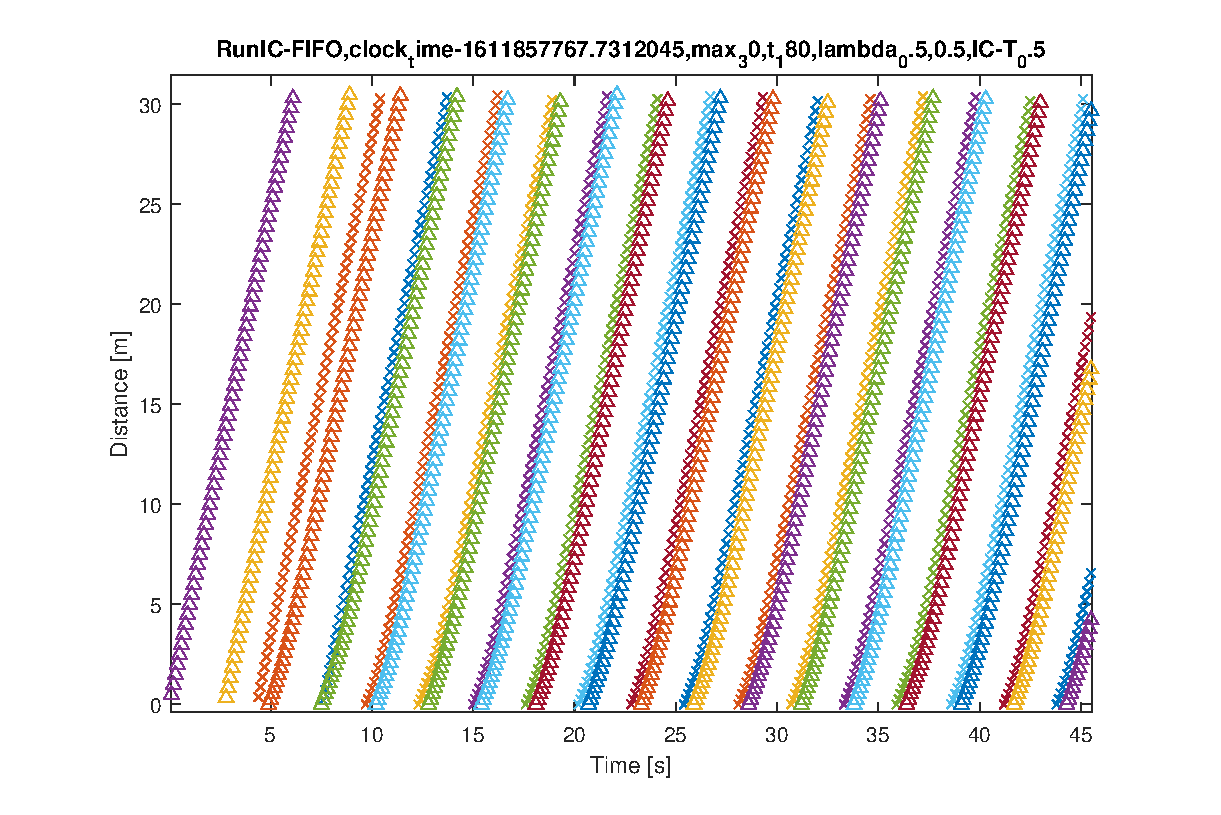
\includegraphics[width=1.0\linewidth]{results_fig/FIFO-HTHL_s-t.eps}
\label{fig:fifo_hlht}
\caption{Position-Time trace for HLHT Scenario under FIFO controller}
\end{figure}
\begin{figure}
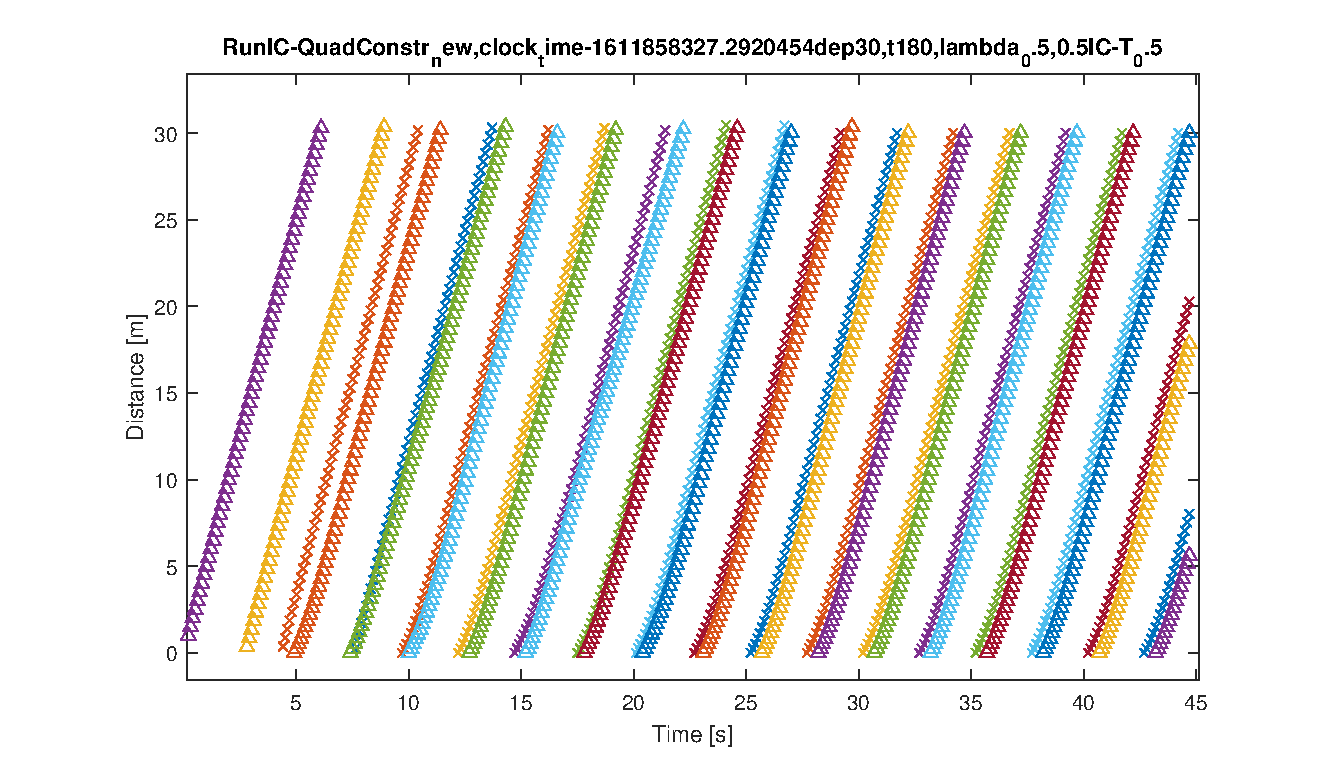
\includegraphics[width=1.0\linewidth]{results_fig/IC-QuadConstr_HLHT_s-t.eps}
\label{fig:quad_hlht}
\caption{Position-Time trace for HLHT Scenario under Quadratic Constraints controller}
\end{figure}
\begin{figure}
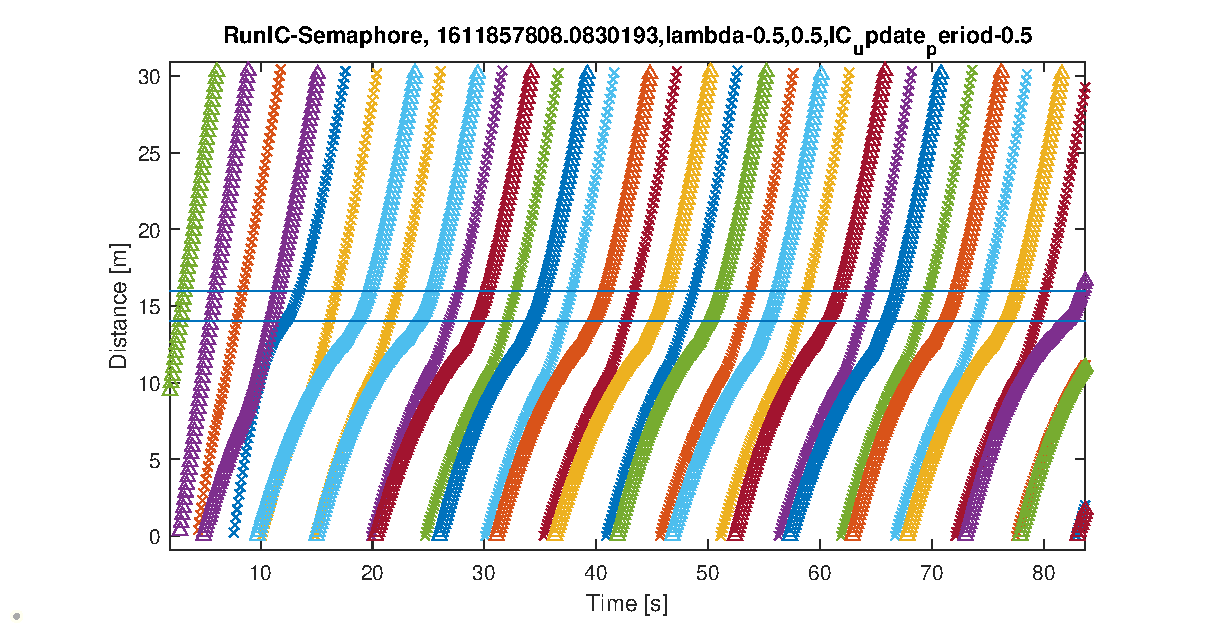
\includegraphics[width=1.0\linewidth]{results_fig/IC-Semaphore-HLHT.eps}
\label{fig:sema_hlht}
\caption{Position-Time trace for HLHT Scenario under Semaphore controller}
\end{figure}
The benefit of modelling the departure time and adjusting speeds in advance is clear from comparing the optimal controllers in Figure \ref{fig:fifo_hlht} and Figure \ref{fig:quad_hlht} with the Semaphore approach in Figure \ref{fig:sema_hlht}. This corresponds to a reduction in delay of 4.85 seconds per vehicle according to Table \ref{tab:results}. 

The two optimal methods are very close, with FIFO achieving a slight improvement in total travel time of 0.6 seconds, but a lower completion time by 0.9 seconds. This discrepancy may occur because the waiting time in the arrival queue is not counted in the total travel time, which should be addressed in further testing. It is more likely the Quadratic constraints achieved a slight improvement in throughput because of the freedom to vary the departure order. However, the departure order in Figure \ref{fig:quad_hlht} turns out to be close to FIFO anyway.

Another avenue of comparison is the energy usage. The semaphore method uses much more energy as the vehicles have to slow down more. Energy usage is not included in the objective for the optimal methods, so the question depends on whether higher average speeds or more acceleration lead to higher losses with our simple motor model.
\begin{figure}
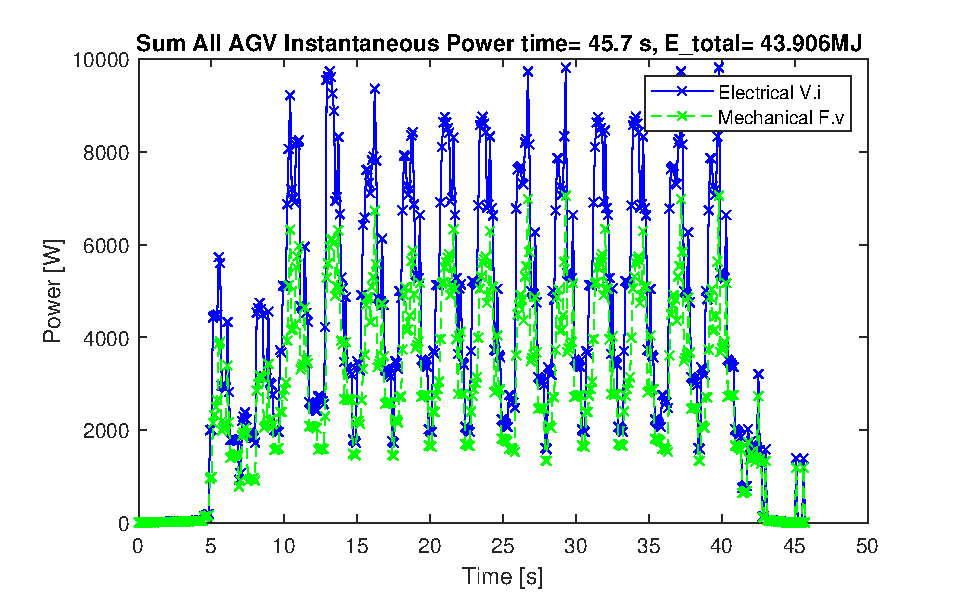
\includegraphics[width=1.0\linewidth]{results_fig/FIFO-HTHL_power_sum-t.eps}
\label{fig:fifo_hlht_pow}
\caption{Power Dissipation-Time trace for HLHT Scenario under FIFO controller}
\end{figure}
\begin{figure}
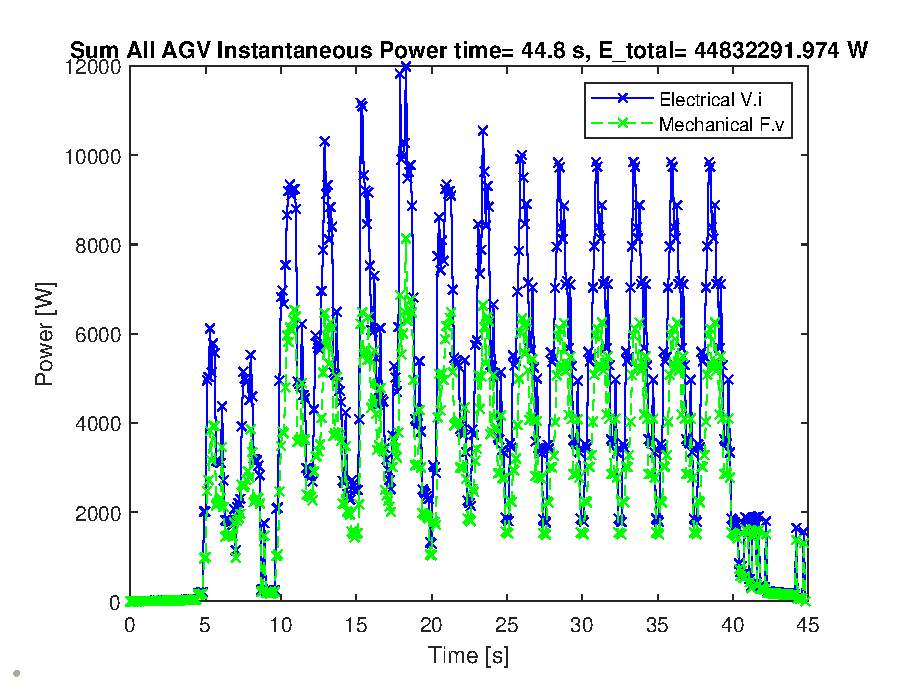
\includegraphics[width=1.0\linewidth]{results_fig/IC-QuadConstr_HLHT_powersum-t.eps}
\label{fig:quad_hlht_pow}
\caption{Power Dissipation-Time trace for HLHT Scenario under Quadratic Constraints controller}
\end{figure}
\begin{figure}
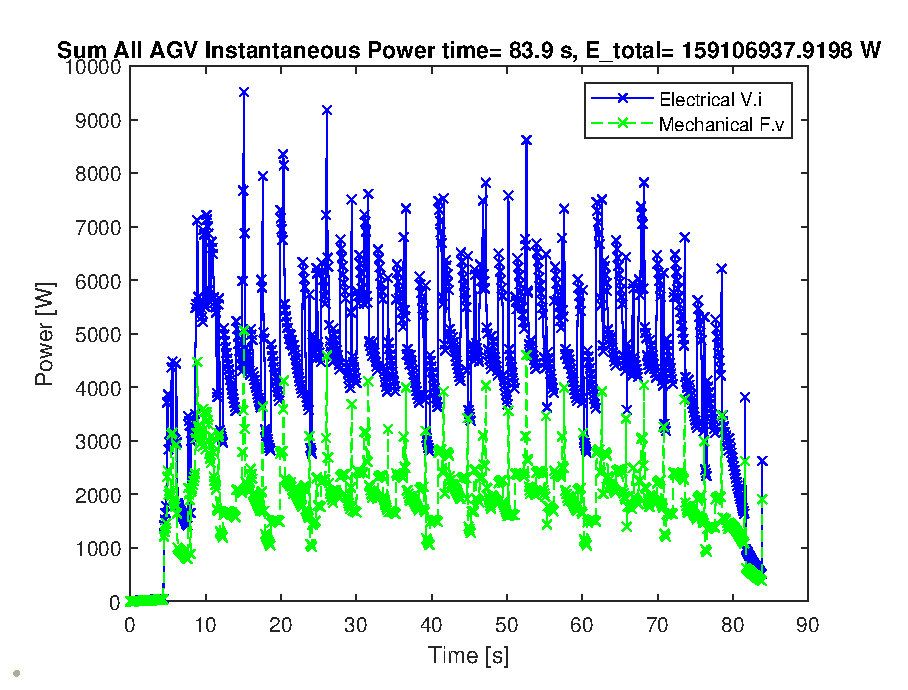
\includegraphics[width=1.0\linewidth]{results_fig/IC-Semaphore-HLHT-powersum.eps}
\label{fig:sema_hlht_pow}
\caption{Power Dissipation-Time trace for HLHT Scenario under Semaphore controller}
\end{figure}

The power consumption increase due to acceleration clearly dominates in Figure \ref{fig:sema_hlht_pow}, as the mechanical power is around 50 percent greater than in either of the optimal runs. This difference is compounded by the reduction in motor efficiency in high acceleration so the resultant increase in electrical poser dissipation is much greater, closer to 200 percent. 

There is still little to distinguish the two optimal approaches. Although unlike the delay, in this case maintaining FIFO order leads to a slight improvement: 43.9 MJ total energy compared to 44.8MJ. A spike in usage at around 18 seconds can be seen in Figure \ref{fig:quad_hlht_pow}, possibly this corresponds to a change in order which leads to lower delay but uses some extra energy. 


\subsection{Impact of Analytical Hessian on Execution Time of Trust Region Method}
The optimization problem with quadratic constraints described in Section \ref{sec:quad} was implemented in Python and solved periodically based on the latest position information at the specified control frequency $f$. The method chosen was 'trust-constr' from the Scipy.Optimize library \cite{scipy}. Trust region methods make use of the exact Semi-Definite Program relaxation for the Trust Region Sub-problem (TRS), of optimizing a non-convex quadratic objective subject to a Euclidean ball constraint, to iteratively solve general non-convex function with non-convex constraints by successive approximation\cite{conn2000trust}. They are likely to be more effective when the general problem has more in common with the TRS and recent methods have been proven to solve variants of that problem in linear time in terms of the input \cite{Wang2019}. Unlike some other general constrained optimization methods in Scipy.Optimize such as SLSQP, 'trust-constr' can make use of the analytical Hessian for the objective and constraints which may be important to exploit the linear objective and quadratic constraints.   

The Hessian must be provided to SciPy.Optimize in the form of a linear combination rather than a stacked matrix. This is to avoid forming the complete Hessian $H \in R^{(n \times np)}$ which may use a significant amount of memory for large problems. Instead, the analytical Hessian function must accept an additional parameter $v \in R^{(1 \times p)}$. This is a vector the same length as the constraints $c_{ineq} \in R^{(1 \times p)}$. The Hessian is returned as a $R^{(n \times n)}$, the weighted sum of pairwise blocks scaled according to $\sum_{i=1}^p v_i H_ij$.
  
With the analytical Hessian the average execution time for the Quadratic Constraints method over the HLHT run in which 30 vehicles passed through the intersection was 0.5251 seconds, varying between 0.0512 seconds to 1.215 seconds as the number of constraints varied from 1 to 6. Without the analytical Hessian of the constraints
Without the analytical constraint  Hessian the mean time taken over the same run was 0.383 seconds, varying between 0.0468 seconds to 7.696 seconds. It is surprising that the worst case time is so much worse and yet the mean time is better. This suggests that in the test data there are more cases with few constraints. It also motivates investigation into the cause of the outlier time. 

The execution time with the FIFO controller never exceeds 15.6 milliseconds on the same set of problems, with the average being 3.6 milliseconds. 

\section{Conclusion}
The advantages of centralized intersection optimization shown by previous authors are supported by our results.  Furthermore we show that enforcing first-in-first-out ordering leads to very similar performance in both delay and energy consumption on a simple intersection comprising two crossed lanes. For this reason the FIFO controller is a promising choice for real world implementation, as it can be solved orders of magnitude faster and captures almost all of the throughput advantage. The next step is to ensure this result holds for more complex intersections, where exploring alternative orderings may be more significant to the objective.    
\chapter{Multiple Intersection Control for Site-wide Motion Co-ordination} 
%\chapter{Dynamic Platooning for Automated Guided Vehicles (AGV)}



\section{Introduction}
AGV typically have their motion restricted to a roadmap connecting pick and drop locations \cite{Cardarelli2017}. This reduces the search space to make conflict free routing of multiple vehicles between different origins and destinations feasible. \cite{Digani2015} proposes a two level decomposition of the problem with the detailed roadmap at the bottom and a higher level abstraction of zones around each intersection above. The conflict avoidance is handled with local information within each zone. The routing decisions are made at high level, utilizing a traffic model where each intersection has a fixed capacity (number of vehicles). 

%\section{INTRODUCTION}
Coordinated conflict-free motion of a number of mobile robots in order to complete a material transfer task is important in the operation of fleets of AGV (Autonomous Guided Vehicles) used in flexible manufacturing and automated warehouses \cite{Vis2006} and \cite{Dotoli2019}. A crucial sub-problem is conflict resolution between multiple AGVs, without control of task assignment or scheduling.

It is shown, in \cite{Digani2019}, that platooning provides superior throughput to the earlier reservation based systems, and that if a solution exists it is optimal, but not that a solution exists on all roadmaps. More importantly a set of conditions which must hold for a solution to exist, is not given. The consensus algorithm in \cite{Tadano2019} also shows improved throughput in concert with a scheduling approach, but does not prove convergence. 
An example of a resolution complete algorithm based on spatial reservation is \cite{Draganjac2020}. Neither per-intersection optimal platooning nor per-vehicle consensus have been proven complete. The lack of guarantees is an important limitation of platooning methods for collision avoidance. The research gap identified is the lack of investigation into the range of motion conflict situations that can be resolved with platooning methods.

\section{Literature Review}
AGV motion coordination can be posed as a variation of the Multiple Vehicle Routing Problem with the addition of challenging spatio-temporal constraints preventing collisions between each vehicle, as well as the usual timing and capacity constraints \cite{Miyamoto2016}. In \cite{Li2017}, solutions are classified into centralized, decentralized and decoupled approaches. Each approach may be either optimal or heuristic based on whether or not they find the global minimum of some objective function. 

It is also possible to classify approaches based on the limitations they place on the state space of each AGV. Most practical methods incorporate both obstacle avoidance constraints and differential motion constraints into some sort of roadmap. This is often a graph with vertices at key points in the reachable state space, connected by edges representing feasible motion between them. The effect of increasing resolution on path quality (measured by reduction in the length of the shortest path) and computation time are studied in \cite{VanDenBerg2005}. 

Interest in centralized methods which plan in the full state space all of the vehicles was renewed by the development of effective numerical tools for operations research able to solve large combinatorial problems to optimality. Notably \cite{Richards2002} found trajectories for aircraft using a linear approximation to the dynamics and obstacle constraints, allowing the use of Mixed Integer Linear Programming. The contribution of \cite{Li2017} is to describe a new centralized, optimal method which scales well, finding a solution to the nonlinear-program for 10 vehicles in just a few seconds using an interior point method. However, size of the combined state space explodes as more vehicles are included so centralized methods are difficult to scale up to large numbers of vehicles.

Many types of decoupled methods have been developed because breaking the problem down into sub-problems is one way to reduce computation time for practical applications. Early methods of this type were based on timed petri nets \cite{Dotoli2004} and agent based models \cite{Singh2002}. Decoupled methods may sacrifice completeness (that a solution is found if one exists) in exchange for reduced average run-time. In \cite{Sanchez2002}, this was shown to cause practical difficulties in the spot-welding task studied. Spot welding requires close formation control of six vehicles, and the decoupled method frequently failed to find a solution. In \cite{Peasgood2008}, decoupled planning (incomplete) is compared with a new multi-phase heuristic, which is complete, for 50 robots on a tunnel map and 150 on an outdoor map. Decoupled planning was consistently faster in execution and produced shorter paths for lower vehicle density however it failed to find any valid paths at all for high vehicle density (25 or more robots in tunnels and 75 or more outdoors). The multi-phase heuristic, being complete, found a solution in every test case. 

More recently, \cite{Yu2013} addressed the lack of optimality in decoupled methods operating on graphs. Optimal conflict-free motion is posed as a large Integer Linear Program. Resolution complete general purpose algorithms are used to solve it for 150 robots in just over 10 seconds. The lattice/graph construction has recently been developed further to ensure kinematic constraints are met and improve coverage of state space around obstacles \cite{Yu2018}. In \cite{Miyamoto2016}, the combined problem of DCFVRP (Dispatch and Conflict-Free Vehicle Routing Problem) for flexible manufacturing is formulated as an integer program and two different decoupled algorithms are presented to solve it: local search and random search. Neither of the proposed algorithms is complete but local search found more valid solutions in the 10 random examples tested, all involving three vehicles.

Decentralized control is another option to decompose large scale problems which take too long to solve centrally \cite{Bakule2008}. Although limiting the information available to each decision maker can make reasoning about collective behavior more difficult, various attempts to decentralize conflict-free routing have been made. 
In the field of conflict free routing for mobile robots, \cite{Draganjac2016} presents a solution which generates a graph representation of the free space - effectively a roadmap - with the property of `collision-avoidability.' This means that every node on the critical path must be at most one move away from a node that does not obstruct the critical path. The critical path is defined as the union of all the shortest paths between pick/drop locations in the roadmap. During decentralized planning, AGVs attempt to reserve `private zones' consisting of the node on the critical path along with all adjacent collision avoidance nodes. Each AGV has an identical roadmap, plans the shortest path to its own goal and negotiates with those nearby based on a numeric priority to reserve the nodes in its own path. An AGV requests those in its path move to their collision avoidance node, and those with a lower priority will do so. Proof is given of correctness, that deadlocks are avoided, but throughput is sub-optimal with low priority vehicles frequently forced to stop and wait. %Another decentralized method based on sequential reservations is given by \cite{Walenta2017}, without the concept of 'private zones' to avoid deadlocks however. 
An alternative decentralized solution, based on a roadmap with two levels of detail is summarized in \cite{Sabattini2018}. Conflict-free routing primarily takes place at the most detailed level, based on prioritized roadmap reservation with local negotiation to guarantee correctness \cite{Digani2014}.  In \cite{Digani2019}, the speed of the approaching AGV is optimized at each intersection in a similar way to centralized intersection platooning. The result is higher throughput as time consuming negotiation is avoided in most cases.      

Congestion effects are represented by link performance functions in the approximate level graph. Intersections have a generalized cost which increases exponentially up to a fixed capacity which identified by parameter tuning, An optimal task scheduling approach based on the Hungarian Algorithm is used to solve the full DCFVRP in \cite{Sabattini2015a} and \cite{Sabattini2018}. Traffic delays are a type of emergent behaviour and modelling is challenging even in a completely automated system. This is the contribution of \cite{Street2020} which introduces the PRT (Probabilistic Reservation Table) to summarize the plans of robots including uncertainty so it can be in task scheduling. This approach is compared with a reservation based centralized planner as a baseline, in a simulation with 5 robots using a low level motion controller from ROS (Robot Operating System) which often fails at when two robots plan interfering paths. Congestion aware planning leads to fewer failures of the low level controller than independent planning but more than centralized planning. A more convincing comparison would be with a congestion aware planner using a deterministic congestion model instead of the PRT, but this is not reported.

Intersection control, based on platooning, is a concept developed for the operation of anticipated CARVs (Connected and Autonomous Road Vehicles). A recent review of approaches for intersection and merging coordination is given in \cite{Rios-Torres2017}. Centralized optimization approaches improve on early ideas like First-Come-First-Served spatial reservation from \cite{Dresner2008} by minimizing fuel consumption, but the rapid increase in state space with larger numbers of vehicles will need to be addressed before large scale adoption. The communication channel connecting every vehicle with the central controller introduces a single point of failure, the reliability effect of which is difficult to evaluate in existing simulations. Moreover there are few CARVs available making a practical experiment unfeasible in most cases. Attempting to address these limitations are decentralized methods such as fuzzy-logic, virtual vehicle platooning and invariant set approaches. Notably the conditions for solutions to exist which minimize energy consumption are given in \cite{Malikopoulos2018}.

Recently \cite{Tadano2019} described an approach to the DCFVRP for flexible manufacturing based on dynamic platooning with vehicle-to-everything messaging and consensus speed control, resulting in a decentralized heuristic solution with some additional rules to ensure correct behavior and avoid deadlocks by adding a reservation protocol for some parts of the roadmap. This was combined with feedback from the queue length at different workstations in a traffic management heuristic. Simulation results show an impressive improvement compared to the first-come-first-served scheduling approach meant to represent industry standard practice.   

A promising approach for intersection control applied to AGV is given in \cite{Digani2019}. As the paths are not modified, only the speed adjusted deadlocks are proved impossible. However, a backup system based on negotiation is still required because the problem is non-convex suggesting a feasible solution may not be found in time for certain roadmap and traffic combinations. The consensus based platooning method for local collision avoidance used in \cite{Tadano2019} is unusual in the AGV domain. That work makes no claims about completeness, but does consider the trivial consensus where all vehicles stop in a deadlock. In \cite{Zhang2018}, a recent system for conflict avoidance based on time headway is shown to significantly reduce intersection crossing time and allow more vehicles to operate in the same floor-space compared to a traditional reservation based strategy. Of these different approaches to platooning for AGV coordination, the quadratic constraints of \cite{Digani2019} are the closest to achieving the certainty required to build a distributed coordination scheme.
%\section{METHODOLOGY}
%
%With existing methods, a backup system is needed to prevent collisions in exceptional cases, as there is no proof of completeness of the main algorithm. A proof might be possible placing certain conditions on the traffic flow or the roadmap layout, but this is left for further work. Instead we focus on simulation to identify situations where convergence is more or less reliable. This will help to identify sites where the potrential throughput benefiits can be realized because the slower fallback option will be needed less often. It may also highlight situations in which current methods frequently fail, and help to inform modified algorithms to address these cases.  

%\begin{figure}[htbp]
%\centerline{\includegraphics[width=1.0\linewidth]{single-track-layout.png}}
%\caption{Single-track grid layout}
%\label{fig:single-track-layout}
%\end{figure}
%%[htbp]
%%\scalebox{0.5}[heightscale]{}
%%\resizebox{1.0\linewidth}{1.0\linewidth} %only for \include{graphics}
%%\centerline{\includegraphics[width=1.0\linewidth]{single-track-layout.png}}
%\begin{figure}[htbp]
%\centerline{\includegraphics[width=1.0\linewidth]{highway-layout.png}}
%\caption{Highway grid layout.}
%\label{fig:highway-layout}
%\end{figure}

%To test the success rate in finding a solution from a variety of initial conditions, we assume all AMR follow their planned trajectory exactly and look for cases where the platooning algorithm did not converge before the intersection, leading to a collision. The trajectory of each AMR must be tracked over time at a relatively high frequency, such as 10hz. Circular bodies of fixed radius can be assumed to make collision checking straightforward. Lateral dynamics can be neglected by assuming the path following controller is successful and tracks the path exactly.  Second order dynamics enable comparison of energy consumption resulting from platooning. Deadlocks and Live-locks can both be checked based on a time threshold for a vehicle to complete a job e.g. the transfer time plus the length of time it would take a vehicle to traverse the entire roadmap. If either is exceeded the simulation state should be recorded for further analysis. 
%
%In order to do this a number of realistic roadmaps are required, along with sensible parameters for vehicle size, acceleration and top speed. These can be estimated based on the literature such as \cite{Boysen2019} and \cite{Dotoli2019}. Important classes of roadmap which may be representative include grids, one-way aisles and two-way aisles.  such as those in Figures \ref{fig:single-track-layout} and \ref{fig:highway-layout}. 


%Conflict avoidance is only one part of the DVFVRP problem, the job assignment method has a profound affect on the frequency and complexity of the motion conflicts which need to be resolved. For this reason it is important to track genuine transfer jobs, assigned to a fixed number of `physical' vehicles (they do not appear and disappear at convenient times and move only according to a second order dynamic model). There is a separate question of which job scheduling algorithm and associated traffic model is best suited to each conflict-resolution method which we will not address here. For simplicity of exposition and ease of reproduction we will use a nearest-first-come-first-served scheduling approach to create traffic for both conflict-resolution methods. This is sufficient that the  number of transfer tasks completed can be tracked in a simulation of `physical' vehicles. Improvement of productivity using a traffic model and the Hungarian algorithm (e.g. \cite{Sabattini2015a}) is left for further work. We know of no reason it would benefit one method in particular.
%\include{Chapters/Chapter_6/Chapter_6_File}


\appendix
\chapter{Optimal Smooth Paths Based on Clothoids for Car-like Vehicles in the Presence of Obstacles}
\label{sec:ijcas}
Paper attached.
\includepdf[pages=-]{2021_192_20-00179-12March2021.pdf}

\section{Bits of \LaTeX advice}

\begin{enumerate}
	\item Do look at the output log and try to understand any errors - they are sometimes important!
	\item In the final pdf, do a search for ? - it is what \LaTeX will give when a reference is missing. Having missing references in your submitted thesis is, at best, embarrassing and potentially a failing matter.
	\item A good quality bib file is important - make sure that entries are consistent in whether journals are abreviated, capitalised and how Author names are presented. A good way to do this is to use Mendeley to import your bib file and then use its doi lookup feature which will re-write your bibliogrpahy entries in a standardised form. You then export the bibliography back oit as a bib file.
	\item Be particularly careful about older papers where the doi may not be easy to track down. Also watch out for JETP Letters that you are being consistent in citing the English language version (or the Russian, but don't mix and match!)
	\item Although \LaTeX guides may show you how to assemble a multi-part fgure from within \LaTeX, it can be hard to make sub-plots appear exactly the same size. We recommend using something like Inkscape to assemble the parts of a figure and lay them out nicely. Be careful if saving to pdf files thatr the fonts are preserved - otherwise you can lose greek symbols.
	\item If preparing figures in Origin, set the plot size to be exactly the right size or exactly double size and then scale fonts and symbols accordingly. Use Origin's ability to copy formatting between graphs to make everything nicely consistent (e.g. frame sizes, thicknesses, coolour schemes, point sizes and shapes).
	\item In general resist the temptation to put [H] when placing figures and tables - in most cases it is better to let \LaTeX work out where to put things. It can get tricky if you have a lot of figures one after another (perhaps a single multi-part figure is what you need?) - the placement option [p] can alos help to move floats to a separate page of figures. See also the \textit{afterpage} package. 
\end{enumerate}
%\chapter{Intersection Control}
%\label{sec:autonomous_robots}
%\includepdf[pages=-]{ar_draft_tsedl.pdf}
%. More appendicies here.
\addcontentsline{toc}{chapter}{References} % Adds References to contents page
%One sectio special { Chapters/Chapter1/SamplingBasedMethods/SamplingBasedPlanningCollection }
\bibliography{References/library,
	Chapters/Chapter_4/roundabouts,
Chapters/Chapter1/2019-08-29-Collection,
Chapters/Chapter_2/icase_draft_references,
Chapters/Chapter_2/simulation, } % References file
\end{document}